%===========================================================
%
% Dedman/Lyle LaTeX Dissertation Template, v.2016
% Structure organized by Ted C. Munger (TCM)
%
%===========================================================
%===========================================================
% BEGIN Document Style
%===========================================================
\documentclass[12pt]{report}

  \usepackage{meta/DL_thesis_v2016}  % TCM Global Style for particular SMU College, e.g. DL_thesis_v2016.sty

  %--------------------------------------------------------------------------------------------------------
% 									LaTeX Package File
%
% TCM Use this file to add, modify, or comment out packages you want to utilize in your Latex project.
%     This file must be included in the main document file.
%--------------------------------------------------------------------------------------------------------

%%%%%%%%%%%%%%%%%%%%%%%%%%%%%%%%%%%%%%%%%%%%%%%%%%%%
\usepackage{algorithm2e}
\usepackage{listings}

% \usepackage{caption}
% \usepackage[caption=false]{subfig}
% \captionsetup[figure]{font={bf,small},skip=0.6\baselineskip,labelsep=period}
\usepackage{subcaption}
% \usepackage[caption=false]{subfig}
% \captionsetup{compatibility=false}

\usepackage{makecell}
\usepackage{float}
% \usepackage{subfloat}
\usepackage{latexsym} 
\usepackage{bytefield}
\usepackage{wrapfig}
\usepackage{mdframed}
%%%%%%%%%%%%%%%%%%%%%%%%%%%%%%%%%%%%%%%%%%%%%%%%%%%%



\usepackage{adjustbox}       % TCM Extends the graphicx package to do trimming and other adjustments.
% \usepackage{algorithm}       % TCM Algorithm block See http://algorithms.berlios.de/
\usepackage{algorithmic}     % TCM Algorithm & Peudocode See http://en.wikibooks.org/wiki/LaTeX/Algorithms_and_Pseudocode
\usepackage{amsmath}         % Need for subequations

%======= new bib package and style
\usepackage[giveninits=true]{biblatex}
\DeclareNameAlias{default}{family-given}

\AtBeginBibliography{%
  \renewcommand*{\mkbibnamelast}[1]{\textsc{#1}}%
  %% commas between authors
  \renewcommand{\multinamedelim}{\addcomma\space}
  \renewcommand{\finalnamedelim}{\addcomma\addspace\textsc{and}\space}
}

\DefineBibliographyStrings{english}{%
 andothers = {\addcomma\addspace\textsc{et\addabbrvspace al}\adddot},
 and = {\textsc{and}}
}
\renewcommand*{\labelnamepunct}{\space\space}

\DeclareFieldFormat
  [article,inbook,incollection,inproceedings,patent,thesis,unpublished]
  {title}{#1}
\renewbibmacro{in:}{%
  \ifentrytype{article}{%
  }{%
    \printtext{\bibstring{in}\intitlepunct}%
  }%
}

\renewbibmacro*{volume+number+eid}{%
  \printfield{volume}%
  \setunit*{\addcomma\space}%
  \printfield{number}%
  \setunit{\addcomma\space}%
  \printfield{eid}}

\DeclareFieldFormat{pages}{#1}

\renewbibmacro*{publisher+location+date}{%
  \printlist{publisher}%
  \setunit*{\addcomma\space}%
  \printlist{location}%
  \setunit*{\addcomma\space}%
  \usebibmacro{date}%
  \newunit}
%======= end new bib
\usepackage{amssymb}        % amssymb-telda and math symbols
\usepackage{booktabs}        % TCM Allows fancy Tables
\usepackage{boxedminipage}   % Boxes around figures
\usepackage{breqn}           % TCM Automatically breaks long equation lines - usually
\usepackage{changepage} 	 % TCM Allows one to temporarily change right and left margins
% \usepackage{cite} 	 		 % TCM Allows improved handling of numeric citations including automatic ordering and ranges of multiple cites
\usepackage{enumitem} 		 % TCM Allows one to easily change the labels for enumerate list
%\usepackage{epsf}           % TCM This EPS file package is greatly depreciated for the graphicx package bundle. Use at own risk.
\usepackage{fancyhdr}
\usepackage{flafter}         % Floats should always appear after their definition
\usepackage[flushleft]{threeparttable}  % TCM This package allows for notes under tables.  Flushleft option flushes the note left margin of table (center is default)
\usepackage{geometry}		 % TCM Allows to customize paper size and margins.
\usepackage{graphicx}        % TCM Extends graphics package for figures. Provides op­tional ar­gu­ments to the \in­clude­graph­ics com­mand
\usepackage{epstopdf}        % TCM Converts eps images to PDF to use in graphicx package.  Must be loaded after graphicx package
\usepackage{longtable}       % TCM Allows for Automatic page breaks for long tables
%\usepackage{jneurosci}       % TCM The jneurosci bibliography style makes use of some commands - for example, \citeauthoryear.  Must include if using named or acmsmall bib style
\usepackage{ltablex}		 % TCM Modifies Tabularx Package by combining properties of tabularx and longtable.
\usepackage[maxfloats=36]{morefloats}      % Latex will handle more floats 18-36
\usepackage{moresize}        % TCM Adds \HUGE and \ssmall font sizes
\usepackage{multirow}        % TCM Allows multirow cells in tables (similar to merge and center in Excel)
%\usepackage{named}           % TCM Bibliography style that allows for more fine-tuned citing. Commands include \cite, \citeauthor, \citeyear and \shortcite (for after you've already used \citeauthor).
\usepackage{outlines}		 % TCM Needed for outlines
\usepackage{rotate}			 % TCM Performs rotations of floating environments (images w/ cations, etc)
\usepackage{rotating}        % Need for sidewaystable
\usepackage{scrextend}		 % TCM package that allows for KOMA-Script classes available for other classes: e.g., labeling lists etc.  See package documentation for further information.
\usepackage{pdflscape}		 % TCM Allows Landscape Page
%%\usepackage{qtree}         % Need for trees
\usepackage{setspace}        % TCM Allows for more intuitive commands for single and double spacing
\usepackage{siunitx}		 % TCM package required to ensure units are typeset properly with numbers e.g. \SI{10}{\kg\m\per\square\s}
\sisetup{output-exponent-marker=\ensuremath{\mathrm{E}}}  % TCM Option allows for Scientific notation of Numbers.  Format is \num{#.####E##}
% \usepackage[superscript]{cite}		  % TCM Makes citations superscript instead of [#]
\usepackage [table]{xcolor}	 % TCM Allows coloring of tables
\usepackage{tabularx}		 % TCM Package which allows paragraphs in Tables
% \usepackage{thumbpdf}		  % TCM Comment out as causes warnings, can easily create thumbs in Adobe if needed.

%===========================================================
% BEGIN Color ToDo Comment Notes for editing
%===========================================================
% \setlength{\marginparwidth}{2cm}
\usepackage[colorinlistoftodos,textwidth=25mm,shadow,backgroundcolor=green]{todonotes}				  % TCM Allows margin comments
\usepackage{marginnote}				  % TCM Require for Todonotes in Align Envionment
  %~~~~~~~~~~~~~~~~~~~~~~~~~~~~~~~~~~~~~~~~~~~~~~~~~~~~~~~~~~~
  % TCM  BEGIN Altering Todonotes Commands to use Marginnote instead of Marginpar to use todonotes in align environment
%~~~~~~~~~~~~~~~~~~~~~~~~~~~~~~~~~~~~~~~~~~~~~~~~~~~~~~~~~~~
     \makeatletter
     \renewcommand{\@todonotes@drawMarginNoteWithLine}{%
     \begin{tikzpicture}[remember picture, overlay, baseline=-0.75ex]%
         \node [coordinate] (inText) {};%
     \end{tikzpicture}%
     \marginnote[{% Draw note in left margin
         \@todonotes@drawMarginNote%
      \@todonotes@drawLineToLeftMargin%
     }]{% Draw note in right margin
         \@todonotes@drawMarginNote%
         \@todonotes@drawLineToRightMargin%
     }%
     }
     \makeatother
       %----------------------------------------------------
       % TCM  BEGIN New Todonotes Command to use single line spacing (sls) in note
       %----------------------------------------------------
       \newcommand{\slstodo}[2][]
       {\todo[caption={#2}, size=\small, #1]{\renewcommand{\baselinestretch}{0.5}\selectfont#2\par}}
       %----------------------------------------------------
       % TCM  END New Todonotes Command to use single spacing in note
       %----------------------------------------------------
       
  %~~~~~~~~~~~~~~~~~~~~~~~~~~~~~~~~~~~~~~~~~~~~~~~~~~~~~~~~~~~
  % TCM  END Altering Todonotes Commands to use Marginnote instead of Marginpar to use todonotes in align 
%~~~~~~~~~~~~~~~~~~~~~~~~~~~~~~~~~~~~~~~~~~~~~~~~~~~~~~~~~~~
%===========================================================
% END Color ToDo Comment Notes for editing
%===========================================================
\usepackage{upquote} %mjz
\usepackage{fancyvrb} %mjz 
\usepackage{verbatim} %mjz       % TCM Verbatim text block
\usepackage{wrapfig}         % Wrap figures
\usepackage{xspace}          % Allows dynamic space in global text variables. This can allow you to just use \newCommandName rather than \newCommandName{}.
% \usepackage [bookmarks=true,backref=page, hyperfigures=true, pdfpagelabels=false] {hyperref}
\usepackage [bookmarks=true, hyperfigures=true, pdfpagelabels=false] {hyperref}
%===========================================================
% BEGIN Hyperlink Setup
%===========================================================
\hypersetup{
									  % TCM Added more precise definition and options for Hyperref package.
									  % TCM Comment out or change hyperref preferences
									  % TCM \hypersetup should be loaded last 
    bookmarksopen=true,				  % True: Open bookmark tree
    bookmarksnumbered=true, 		  % True: put section numbers in bookmarks
    breaklinks=true,				  % True: split the url over multiple lines
%    draft=true,						  % True: do not do any hyper linking
    filecolor=magenta, 				  % Color of file links
    citecolor=blue, 				  % Color of links to bibliography
    colorlinks=true, 				  % False: boxed links; true: colored links
    linkcolor=blue, 				  % Color of internal links
    linktocpage=true, 				  % True: Makes the page number of TOC the link vs the text
%    pagebackref=true,				  % True: Links references back to referring page
    pdfnewwindow=true,         		  % True: URL links in new window
    plainpages=false, 				  % True: do page number anchors as plain Arabic
    pdffitwindow=false,        		  % Window fit to page when opened
    pdfmenubar=true,           		  % Show Acrobat menu
    pdfstartview={FitH},       		  % Fits the width of the page to the window
    pdftoolbar=true, 				  % Show Acrobat toolbar
    pdfauthor={Author}, 			  % Author in PDF document properties
    pdfcreator={Author}, 			  % Creator of the document in PDF document properties
    pdfkeywords={Keyword1} {Keyword2} {Keyword3} {Keyword4} {Author}, % List of keywords in PDF document properties
    pdfproducer={Producer}, 		  % Producer of the document in PDF document properties
    pdfsubject={Subject},   % Subject of the document in PDF document properties
    pdftitle={Title of Dissertation}, % Title in PDF document properties
    unicode=false,             		  % Non-Latin characters in Acrobat bookmarks
    urlcolor=cyan 					  % Color of external links
}
%===========================================================
% END Hyperlink Setup
%===========================================================
\usepackage{bookmark}		 		  % TCM Eliminates Warning Bookmark level greater than one.  Must be loaded after Hyperref

               % Packages File

  \geometry{letterpaper, margin=1in} % TCM Dedman/Lyle Standard 2016


  \linespread{1.6}
  \setcounter{secnumdepth}{4} % TCM Sets number subsections
  \setcounter{tocdepth}{4}    % TCM Set the number of subsections in TOC
  
   \urlstyle{same} % TCM Set URL style to same font as text verses mono-spaced, i.e., courier

%===========================================================
% END Document Style
%===========================================================
%===========================================================
% BEGIN Insert Custom Commands
%===========================================================
  %======================================================================
% Custom Commands  Inital Creation TCM 2015
%======================================================================
% Use this document to place all of your global new commands
%======================================================================

%======================================================================
% BEGIN SMU Custom Commands
%======================================================================
% The many of the following commands were originally in the smu_thesis.sty
% file. Commands and comments were moved here to make style file more about
% document style. While custom environments can technically be considered 
% style, the student created environments are included here to simplify
% the style file. Often these commands were created by students over the
% years and placed in the style file.  The commands have not been 
% verified and can be obsolete LaTeX commands. The Commands can be used 
% or ignored. 
%======================================================================
%----------------------------------------------------------------------
% BEGIN TCM Commands to set formatting for Paragraph section to have line
%           feed after heading & Numbered. This custom command makes
%           \paragraph, in essence, a form of \subsubsubsection.
%           Uncomment to use.
%----------------------------------------------------------------------
%  \makeatletter
%  \renewcommand\paragraph{\@startsection{paragraph}{4}{\z@}%
%    {-3.25ex\@plus -1ex \@minus -.2ex}%
%    {1.5ex \@plus .2ex}%
%    {\normalfont\normalsize\bfseries}}
%  \makeatother
%----------------------------------------------------------------------
% END of Commands to set formatting for Paragraph section to have line
%       feed after heading TCM
%----------------------------------------------------------------------
%----------------------------------------------------------------------
% BEGIN Shortcuts to insert calligraphic letters in Math Mode Only
%----------------------------------------------------------------------
\newcommand{\cA}{{\mathcal A}}
\newcommand{\cB}{{\mathcal B}}
\newcommand{\cC}{{\mathcal C}}
\newcommand{\cD}{{\mathcal D}}
\newcommand{\cE}{{\mathcal E}}
\newcommand{\cF}{{\mathcal F}}
\newcommand{\cG}{{\mathcal G}}
\newcommand{\cH}{{\mathcal H}}
\newcommand{\cI}{{\mathcal I}}
\newcommand{\cJ}{{\mathcal J}}
\newcommand{\cK}{{\mathcal K}}
\newcommand{\cL}{{\mathcal L}}
\newcommand{\cM}{{\mathcal M}}
\newcommand{\cN}{{\mathcal N}}
\newcommand{\cO}{{\mathcal O}}
\newcommand{\cP}{{\mathcal P}}
\newcommand{\cQ}{{\mathcal Q}}
\newcommand{\cR}{{\mathcal R}}
\newcommand{\cS}{{\mathcal S}}
\newcommand{\cT}{{\mathcal T}}
\newcommand{\cU}{{\mathcal U}}
\newcommand{\cV}{{\mathcal V}}
\newcommand{\cW}{{\mathcal W}}
\newcommand{\cX}{{\mathcal X}}
\newcommand{\cY}{{\mathcal Y}}
\newcommand{\cZ}{{\mathcal Z}}
% Lower case caligraphy letters
\newcommand{\cw}{{\mathcal w}}
%----------------------------------------------------------------------
% END Shortcuts to insert calligraphic letters in Math Mode Only
%----------------------------------------------------------------------
%----------------------------------------------------------------------
% BEGIN Shortcuts to insert boldface letters 
%----------------------------------------------------------------------
\newcommand{\bA}{{\bf A}}
\newcommand{\bB}{{\bf B}}
\newcommand{\bC}{{\bf C}}
\newcommand{\bD}{{\bf D}}
\newcommand{\bE}{{\bf E}}
\newcommand{\bF}{{\bf F}}
\newcommand{\bG}{{\bf G}}
\newcommand{\bH}{{\bf H}}
\newcommand{\bI}{{\bf I}}
\newcommand{\bJ}{{\bf J}}
\newcommand{\bK}{{\bf K}}
\newcommand{\bL}{{\bf L}}
\newcommand{\bM}{{\bf M}}
\newcommand{\bN}{{\bf N}}
\newcommand{\bO}{{\bf O}}
\newcommand{\bP}{{\bf P}}
\newcommand{\bQ}{{\bf Q}}
\newcommand{\bR}{{\bf R}}
\newcommand{\bS}{{\bf S}}
\newcommand{\bT}{{\bf T}}
\newcommand{\bU}{{\bf U}}
\newcommand{\bV}{{\bf V}}
\newcommand{\bW}{{\bf W}}
\newcommand{\bX}{{\bf X}}
\newcommand{\bY}{{\bf Y}}
\newcommand{\bZ}{{\bf Z}}
%----------------------------------------------------------------------
% END Shortcuts to insert boldface letters 
%----------------------------------------------------------------------
%----------------------------------------------------------------------
% BEGIN Shortcuts to insert overline symbols in Math Mode Only
%----------------------------------------------------------------------
\newcommand{\oA}{{\overline A}}
\newcommand{\oB}{{\overline B}}
\newcommand{\oC}{{\overline C}}
\newcommand{\oD}{{\overline D}}
\newcommand{\oE}{{\overline E}}
\newcommand{\oF}{{\overline F}}
\newcommand{\oG}{{\overline G}}
\newcommand{\oH}{{\overline H}}
\newcommand{\oI}{{\overline I}}
\newcommand{\oJ}{{\overline J}}
\newcommand{\oK}{{\overline K}}
\newcommand{\oL}{{\overline L}}
\newcommand{\oM}{{\overline M}}
\newcommand{\oN}{{\overline N}}
\newcommand{\oO}{{\overline O}}
\newcommand{\oP}{{\overline P}}
\newcommand{\oQ}{{\overline Q}}
\newcommand{\oR}{{\overline R}}
\newcommand{\oS}{{\overline S}}
\newcommand{\oT}{{\overline T}}
\newcommand{\oU}{{\overline U}}
\newcommand{\oV}{{\overline V}}
\newcommand{\oW}{{\overline W}}
\newcommand{\oX}{{\overline X}}
\newcommand{\oY}{{\overline Y}}
\newcommand{\oZ}{{\overline Z}}
% Lower case overline
\newcommand{\ovd}{{\overline d}}
\newcommand{\ove}{{\overline e}}
\newcommand{\ovf}{{\overline f}}
\newcommand{\ovg}{{\overline g}}
\newcommand{\ovh}{{\overline h}}
\newcommand{\ovi}{{\overline i}}
%----------------------------------------------------------------------
% END Shortcuts to insert overline symbols in Math Mode Only
%----------------------------------------------------------------------
%----------------------------------------------------------------------
% BEGIN Shortcuts to insert vector symbols in Math Mode Only
%----------------------------------------------------------------------
\newcommand{\vS}{{\vec S}}
\newcommand{\vT}{{\vec T}}
\newcommand{\vU}{{\vec U}}
\newcommand{\vV}{{\vec V}}
\newcommand{\vW}{{\vec W}}
\newcommand{\vX}{{\vec X}}
\newcommand{\vY}{{\vec Y}}
\newcommand{\vZ}{{\vec Z}}
% Lower case vectors
\newcommand{\vs}{{\vec s}}
\newcommand{\vt}{{\vec t}}
\newcommand{\vu}{{\vec u}}
\newcommand{\vv}{{\vec v}}
\newcommand{\vw}{{\vec w}}
\newcommand{\vx}{{\vec x}}
%----------------------------------------------------------------------
% END Shortcuts to insert vector symbols in Math Mode Only
%----------------------------------------------------------------------
%----------------------------------------------------------------------
% BEGIN Misc. Commands defined by students
%----------------------------------------------------------------------
\newcommand{\myqed}{\vspace{-1.1cm} \qed \vspace{0.9cm}}
\newcommand{\qed}{\mbox{$\ \Box$}}
\newcommand{\lqed}{\qed\vspace{.1in}}
\newcommand{\nf}{{\mbox{$\sim$}}}
\newcommand{\wt}{\mbox{$\widehat{T}$}}
\newcommand{\as}{\mbox{$/\hspace{-2mm}>$}}
\newcommand{\equi}{\mbox{$\leftrightarrow$}}
\newcommand{\myeq}{\mbox{$\leftrightarrow$}}
%\newcommand{\tab}{\hspace*{4em}}
%\newcommand{\ind}{\hspace*{2em}}
%\newcommand{\mif}{\mbox{ :- }}
%\newcommand{\dd}{\mbox{$\bullet$}}
\newcommand{\dd}{\mbox{\ $\mid$\ }}

\newcommand{\ind}{\hspace*{2.0em}}
\newcommand{\tab}{\hspace*{4em}}

\newcommand{\myp}{\protect{$+$}}
\newcommand{\mypp}[1]{\protect{${#1}$}}
\newcommand{\myf}[2]{\protect{\ \(\frac{\mbox{\rm #1}}{\mbox{\rm #2}}\)}\ }
\newcommand{\myup}{\protect{$ \uparrow$}}
\newcommand{\scc}[1]{\protect{\ \ \ $ SCC = {#1} $}}

% \newcommand{\twoheadrightarrow}{{\rightarrow \hspace{-0.3cm} \rightarrow \hspace{0.2cm}}}

\newcommand{\chap}[1]{\chapter{\protect{\bf {#1}}}}
\newcommand{\mytab}{\hspace*{13em}}
\newcommand{\bleft}{\left \{\ }
\newcommand{\bright}{\ \right \}}
\newcommand{\sind}{ \ \ \ }
\newcommand{\mand}{ \ \&\ }
\newcommand{\mif}{\mbox{\ :-\ }}
%%%\newcommand{\nf}{\sim}
\newcommand{\posI}{$I^+$}
\newcommand{\negI}{$I^-$}
%\newcommand{\AST}{$AST(P)$}
\newcommand{\Ip}[1]{${\mathcal I}_{#1}$}
\newcommand{\II}[1]{${\mathcal I}({#1})$}
%\newcommand{\HU}[1]{${\mathcal HU}_{#1}$}
%\newcommand{\US}{${\mathcal US}$}
%\newcommand{\HB}[1]{${\mathcal HB}_{#1}$}
%----- chen  -----------------
%\newcommand{\emptyset}{\phi}
\newcommand{\cUS}{{\mathcal US}}
\newcommand{\cHU}{{\mathcal HU}}
\newcommand{\cHB}{{\mathcal HB}}
\newcommand{\cUC}{{\mathcal UC}s}
\newcommand{\cBody}{{\mathcal B}ody}
\newcommand{\wA}{\widetilde{\rm A}}
\newcommand{\LF}{${\mathcal LF}$}
\newcommand{\DI}{DI^+ \cup DI^-}
\newcommand{\AI}{AI^+ \cup AI^-}
\newcommand{\Asp}{\tt asp}
\newcommand{\Aspt}[1]{${\tt asp}({#1})$}
\newcommand{\BP}[1]{${\mathcal BP}({#1})$}
\newcommand{\myarrow}{-\hspace*{-0.23cm}-\hspace*{-0.23cm}-\hspace*{-0.23cm}\longrightarrow}
\newcommand{\nedge}{\rightarrow\hspace*{-0.39cm}{\prime} \hspace*{0.29cm}}
\newcommand{\jmp}[1] {\hspace*{0.3in}{#1}\hspace*{0.3in}}
\newcommand{\Aro}[1]{\stackrel{#1}\longrightarrow}
\newcommand{\MyAro}[1]{\stackrel{#1}\myarrow}
\newcommand{\MyLoAro}[1]{\stackrel{#1}{-\hspace*{-0.23cm}-\hspace*{-0.23cm}\myarrow}}

%----- For figures  ---------------------------------------------------

\newcommand{\myfigureold}[3]{ \begin{figure}[tbp]
  \begin{center}
   \fbox{
    \begin{minipage}[t]{5.7in}
    \rule[-.1cm]{0cm}{0.5cm} % changed by saeed to 0.01cm was 0.5cm
    \centerline{\psfig{#1}}
    \end{minipage}
    }
    \end{center}
       \caption{#2} \label{#3} \vskip -0.14in \end{figure} } % changed by saeed was -0.14 changed to -0.01in

\newcommand{\mytabfig}[3]{ \begin{figure}[tbp]
  \begin{center}
   \fbox{
    \begin{minipage}[t]{5.7in}
    \rule[-.1cm]{0cm}{0.5cm} % changed by saeed to 0.01cm was 0.5cm
#1
    \end{minipage}
        }
        \end{center}
       \caption{#2} \label{#3} \vskip -0.14in \end{figure} } % changed by saeed was -0.14 changed to -0.01in

\newcommand{\myfigure}[3]{ \begin{figure}[tbp]
    \begin{center}
    #1
    \end{center}
    \caption{#2} \label{#3} \vskip -0.14in \end{figure} } % changed by saeed was -0.14 changed to -0.01in

\newcommand{\mytable}[3]{ \begin{table}[tbp]
  \begin{center}
  \caption{#2}
    #1
  \label{#3} \vskip -0.01in \end{center} \end{table} }

\newcommand{\myendfig}{\vskip -0.14in \end{figure} } % changed by saeed was -0.14in changed to -0.01in
\newcommand{\myendtab}{\vskip -0.01in \end{table} }

%----------------- theorem definitions --------------------------------

\newtheorem{ex}{Example}[chapter]
\newtheorem{theor}{Theorem}[chapter]
\newtheorem{mtd}{Method}[chapter]
\newtheorem{mydef}{Definition}[chapter]
%\newtheorem{mylem}{Lemma}[chapter]
\newtheorem{mylem}[theor]{Lemma}

%\newtheorem{algorithm}{Algorithm}[chapter]
%\newtheorem{corollary}[theorem]{Corollary}
%\newtheorem{proposition}{Proposition}[section]
%\newtheorem{remark}{Remark}[section]

%----------------------------------------------------------------------
%\font\pf=rpcrr at 11pt    % TCM Comment out if using Overleaf.com
%\font\spf=rpcrr at 11pt   % TCM Comment out if using Overleaf.com
%----------------------------------------------------------------------

%-------------------- environment definitions -------------------------
\newenvironment{example}{\begin{ex} \rm}{\hfill \qed \end{ex}}
\newenvironment{theorem}{\begin{theor}}{ \end{theor}}
\newenvironment{method}{\begin{mtd} \rm}{\hfill \qed \end{mtd}}
\newenvironment{definition}{\begin{mydef} \rm}{\hfill \qed \end{mydef}}
%\newenvironment{lemma}{\begin{mylem} \rm}{\hfill \qed \end{mylem}}
\newenvironment{lemma}{\begin{mylem}}{ \end{mylem}}

\newenvironment{vers}{\vspace{-0.1cm} \begin{verse}}{\vspace{-0.1cm} \end{verse}}
\newenvironment{vers2}{\vspace{-0.2cm} \begin{verse}}{\vspace{-0.1cm} \end{verse}}

\newenvironment{proof}[0]{\vspace{0.3cm}\noindent {\bf Proof:} \rm }{\hfill \lqed}
\newenvironment{proof-of}[1]{\noindent {\bf Proof of #1:}}{\hfill \lqed}
%----------------------------------------------------------------------
% END Misc. Commands defined by students
%----------------------------------------------------------------------
%======================================================================
% END SMU Custom Commands
%======================================================================        %  File of global custom commands
  
\lstset
{ %Formatting for code in appendix
    language=prolog,
    basicstyle=\footnotesize,
    numbers=left,
    stepnumber=1,
    showstringspaces=false,
    tabsize=1,
    breaklines=true,
    breakatwhitespace=false,
}
  
  % include syntax styles for code listings

% yaml lang style based on: https://tex.stackexchange.com/questions/152829/how-can-i-highlight-yaml-code-in-a-pretty-way-with-listings/152856#152856

\newcommand\YAMLcolonstyle{\color{red}\mdseries}
\newcommand\YAMLkeystyle{\color{black}\bfseries}
\newcommand\YAMLvaluestyle{\color{blue}\mdseries}

\makeatletter
\newcommand\language@yaml{yaml}

\expandafter\expandafter\expandafter\lstdefinelanguage
\expandafter{\language@yaml}
{
  keywords={true,false,null,y,n},
  keywordstyle=\color{darkgray}\bfseries,
  basicstyle=\linespread{0.9}\YAMLkeystyle\footnotesize, % assuming a key comes first
  frame=single,
  framesep=\fboxsep,
  framerule=\fboxrule,
  rulecolor=\color{black},
  xleftmargin=\dimexpr\fboxsep,
  xrightmargin=\dimexpr\fboxsep,
  tabsize=2,
  numberstyle=\small,
  columns=flexible,
  breaklines=true,
  sensitive=false,
  comment=[l]{\#},
  morecomment=[s]{/*}{*/},
  commentstyle=\color{purple}\ttfamily,
  stringstyle=\YAMLvaluestyle\ttfamily,
  moredelim=[l][\color{orange}]{\&},
  moredelim=[l][\color{magenta}]{*},
  moredelim=**[il][\YAMLcolonstyle{:}\YAMLvaluestyle]{:},   % switch to value style at :
  morestring=[b]',
  morestring=[b]",
  literate =    {---}{{\ProcessThreeDashes}}3
                {>}{{\textcolor{red}\textgreater}}1     
                {|}{{\textcolor{red}\textbar}}1 
                {\ -\ }{{\mdseries\ -\ }}3,
}
% switch to key style at EOL
\lst@AddToHook{EveryLine}{\ifx\lst@language\language@yaml\YAMLkeystyle\fi}
\makeatother
\newcommand\ProcessThreeDashes{\llap{\color{cyan}\mdseries-{-}-}}


% \usepackage[top=1in]{geometry}
\usepackage{textcomp}
\usepackage{listings}
%\usepackage{minted}      % (requires -shell-escape)
\usepackage{xcolor}
\usepackage{filecontents}

% --- ugly internals for language definition ---
%
\makeatletter

% initialisation of user macros
\newcommand\PrologPredicateStyle{}
\newcommand\PrologVarStyle{}
\newcommand\PrologAnonymVarStyle{}
\newcommand\PrologAtomStyle{}
\newcommand\PrologOtherStyle{}
\newcommand\PrologCommentStyle{}

% useful switches (to keep track of context)
\newif\ifpredicate@prolog@
\newif\ifwithinparens@prolog@

% save definition of underscore for test
\lst@SaveOutputDef{`_}\underscore@prolog

% local variables
\newcount\currentchar@prolog

\newcommand\@testChar@prolog%
{%
  % if we're in processing mode...
  \ifnum\lst@mode=\lst@Pmode%
    \detectTypeAndHighlight@prolog%
  \else
    % ... or within parentheses
    \ifwithinparens@prolog@%
      \detectTypeAndHighlight@prolog%
    \fi
  \fi
  % Some housekeeping...
  \global\predicate@prolog@false%
}

% helper macros
\newcommand\detectTypeAndHighlight@prolog
{%
  % First, assume that we have an atom.
  \def\lst@thestyle{\PrologAtomStyle}%
  % Test whether we have a predicate and modify the style accordingly.
  \ifpredicate@prolog@%
    \def\lst@thestyle{\PrologPredicateStyle}%
  \else
    % Test whether we have a predicate and modify the style accordingly.
    \expandafter\splitfirstchar@prolog\expandafter{\the\lst@token}%
    % Check whether the identifier starts by an underscore.
    \expandafter\ifx\@testChar@prolog\underscore@prolog%
      % Check whether the identifier is '_' (anonymous variable)
      \ifnum\lst@length=1%
        \let\lst@thestyle\PrologAnonymVarStyle%
      \else
        \let\lst@thestyle\PrologVarStyle%
      \fi
    \else
      % Check whether the identifier starts by a capital letter.
      \currentchar@prolog=65
      \loop
        \expandafter\ifnum\expandafter`\@testChar@prolog=\currentchar@prolog%
          \let\lst@thestyle\PrologVarStyle%
          \let\iterate\relax
        \fi
        \advance \currentchar@prolog by 1
        \unless\ifnum\currentchar@prolog>90
      \repeat
    \fi
  \fi
}
\newcommand\splitfirstchar@prolog{}
\def\splitfirstchar@prolog#1{\@splitfirstchar@prolog#1\relax}
\newcommand\@splitfirstchar@prolog{}
\def\@splitfirstchar@prolog#1#2\relax{\def\@testChar@prolog{#1}}

% helper macro for () delimiters
\def\beginlstdelim#1#2%
{%
  \def\endlstdelim{\PrologOtherStyle #2\egroup}%
  {\PrologOtherStyle #1}%
  \global\predicate@prolog@false%
  \withinparens@prolog@true%
  \bgroup\aftergroup\endlstdelim%
}

% language name
\newcommand\lang@prolog{Prolog-pretty}
% ``normalised'' language name
\expandafter\lst@NormedDef\expandafter\normlang@prolog%
  \expandafter{\lang@prolog}

% language definition
\expandafter\expandafter\expandafter\lstdefinelanguage\expandafter%
{\lang@prolog}
{%
  language            = Prolog,
  keywords            = {},      % reset all preset keywords
  showstringspaces    = false,
  alsoletter          = (,
%   alsoother           = @$,
%   moredelim           = **[is][\beginlstdelim{(}{)}]{(}{)},
  MoreSelectCharTable =
    \lst@DefSaveDef{`(}\opparen@prolog{\global\predicate@prolog@true\opparen@prolog},
}

% Hooking into listings to test each ``identifier''
\newcommand\@ddedToOutput@prolog\relax
\lst@AddToHook{Output}{\@ddedToOutput@prolog}

\lst@AddToHook{PreInit}
{%
  \ifx\lst@language\normlang@prolog%
    \let\@ddedToOutput@prolog\@testChar@prolog%
  \fi
}

\lst@AddToHook{DeInit}{\renewcommand\@ddedToOutput@prolog{}}

\makeatother
%
% --- end of ugly internals ---


% --- definition of a custom style similar to that of Pygments ---
% custom colors
\definecolor{PrologPredicate}{RGB}{000,031,255}
\definecolor{PrologVar}      {RGB}{024,021,125}
\definecolor{PrologAnonymVar}{RGB}{000,127,000}
\definecolor{PrologAtom}     {RGB}{186,032,032}
\definecolor{PrologComment}  {RGB}{063,128,127}
\definecolor{PrologOther}    {RGB}{000,000,000}

% redefinition of user macros for Prolog style
\renewcommand\PrologPredicateStyle{\color{PrologPredicate}}
\renewcommand\PrologVarStyle{\color{PrologVar}}
\renewcommand\PrologAnonymVarStyle{\color{PrologAnonymVar}}
\renewcommand\PrologAtomStyle{\color{PrologAtom}}
\renewcommand\PrologCommentStyle{\itshape\color{PrologComment}}
\renewcommand\PrologOtherStyle{\color{PrologOther}}

% custom style definition 
\lstdefinestyle{datalog}
{
  language     = Prolog-pretty,
  upquote      = true,
  stringstyle  = \PrologAtomStyle,
  commentstyle = \PrologCommentStyle,
  literate     =
    {:-}{{\PrologOtherStyle :-}}2
    {,}{{\PrologOtherStyle ,}}1
    {.}{{\PrologOtherStyle .}}1
}

% global settings
\lstset
{
  captionpos = below,
  frame      = single,
  columns    = fullflexible,
  basicstyle = \ttfamily\footnotesize,
}

% write some sample code to an external file
% \begin{filecontents*}{sample.pl}
% somePredicate(_, B) :-
%     arbitraryPredicate(A, _variable, 1, 2),
%     predicateWithAtom(someAtom),
%     anotherPredicate(B, someAtom, myPredicate(A, _)),
%     findall(X, ('testString'(X), myPredicate(A, X)), L1),
%     member(A, L1),
%     !.
%     /*
%     block comment: blah blah blah
%     */
%     % to-end-of-line comment: blah blah blah
% \end{filecontents*}


\definecolor{delim}{RGB}{20,105,176}
\definecolor{numb}{RGB}{106, 109, 32}
\definecolor{string}{rgb}{0.64,0.08,0.08}

\lstdefinelanguage{json}{
    numbers=left,
    numberstyle=\small,
    frame=single,
    rulecolor=\color{black},
    showspaces=false,
    showtabs=false,
    breaklines=true,
    postbreak=\raisebox{0ex}[0ex][0ex]{\ensuremath{\color{gray}\hookrightarrow\space}},
    breakatwhitespace=true,
    basicstyle=\linespread{0.8}\ttfamily\small,
    upquote=true,
    morestring=[b]",
    stringstyle=\color{string},
    literate=
     *{0}{{{\color{numb}0}}}{1}
      {1}{{{\color{numb}1}}}{1}
      {2}{{{\color{numb}2}}}{1}
      {3}{{{\color{numb}3}}}{1}
      {4}{{{\color{numb}4}}}{1}
      {5}{{{\color{numb}5}}}{1}
      {6}{{{\color{numb}6}}}{1}
      {7}{{{\color{numb}7}}}{1}
      {8}{{{\color{numb}8}}}{1}
      {9}{{{\color{numb}9}}}{1}
      {\{}{{{\color{delim}{\{}}}}{1}
      {\}}{{{\color{delim}{\}}}}}{1}
      {[}{{{\color{delim}{[}}}}{1}
      {]}{{{\color{delim}{]}}}}{1},
}


% \colorlet{punct}{red!60!black}
% \definecolor{background}{HTML}{EEEEEE}
% \definecolor{delim}{RGB}{20,105,176}
% \colorlet{numb}{magenta!60!black}

% \lstdefinelanguage{json}{
%     basicstyle=\linespread{0.8}\normalfont\ttfamily,
%     numbers=left,
%     numberstyle=\scriptsize,
%     stepnumber=1,
%     numbersep=8pt,
%     showstringspaces=false,
%     breaklines=true,
%     frame=lines,
%     backgroundcolor=\color{background},
%     literate=
%      *{0}{{{\color{numb}0}}}{1}
%       {1}{{{\color{numb}1}}}{1}
%       {2}{{{\color{numb}2}}}{1}
%       {3}{{{\color{numb}3}}}{1}
%       {4}{{{\color{numb}4}}}{1}
%       {5}{{{\color{numb}5}}}{1}
%       {6}{{{\color{numb}6}}}{1}
%       {7}{{{\color{numb}7}}}{1}
%       {8}{{{\color{numb}8}}}{1}
%       {9}{{{\color{numb}9}}}{1}
%       {:}{{{\color{punct}{:}}}}{1}
%       {,}{{{\color{punct}{,}}}}{1}
%       {\{}{{{\color{delim}{\{}}}}{1}
%       {\}}{{{\color{delim}{\}}}}}{1}
%       {[}{{{\color{delim}{[}}}}{1}
%       {]}{{{\color{delim}{]}}}}{1},
% }
%===========================================================
% END Insert Custom Commands
%===========================================================
%===========================================================
% BEGIN Code to Minimize Error Warnings
%===========================================================
%-----------------------------------------------------------
% BEGIN Reduce compile warnings for overfull and underfull hboxes & vboxes
%       Adjust up or down to fit your specific needs TCM
%-----------------------------------------------------------
  \hbadness=50000
  \vbadness=50000
  \hfuzz=150pt
%-----------------------------------------------------------  
% END Reduce compile warnings for overfull and underfull hboxes TCM
%-----------------------------------------------------------
%-----------------------------------------------------------
% BEGIN eliminate compile warnings for noindent hfill hbox in PDF bookmarks TCM
%-----------------------------------------------------------
  \pdfstringdefDisableCommands{
  \def\hbox{ }                      % hyperref (temporarily) changes \hbox to a space in this context.
  \def\hfill{ }                     % hyperref (temporarily) changes \hfill to a space in this context.
  \def\noindent{ }                  % hyperref (temporarily) changes \noindent to a space in this context.
  \def\hskip{ }                     % hyperref (temporarily) changes \hskip to a space in this context.
  }
%-----------------------------------------------------------
% END eliminate compile warnings for noindent hfill hbox in PDF bookmarks TCM
%-----------------------------------------------------------
%===========================================================
% END Code to Minimize Error Warnings
%===========================================================
%===========================================================

% \thesisdraft                       % TCM uncomment if want draft printing

% %============
% % begin texcount stats 
% %=============

% %% You can pass in your own texcount params, e.g. -chinese to turn on Chinese mode, or -char to do a character count instead (which does NOT include spaces!)
% %%% http://app.uio.no/ifi/texcount/documentation.html

% %% To include references. DO NOT USE WITH BIBLATEX 
% %TC:incbib

% %% To include tabulars in main text count.
% %TC:group table 0 1
% %TC:group tabular 1 1

% \newcommand{\detailtexcount}[1]{%
%   \immediate\write18{texcount -merge -sum -q #1.tex output.bbl > #1.wcdetail }%
%   \verbatiminput{#1.wcdetail}%
% }

% \newcommand{\quickwordcount}[1]{%
%   \immediate\write18{texcount -1 -sum -merge -q #1.tex output.bbl > #1-words.sum }%
%   \input{#1-words.sum} words%
% }

% %   -sum, -sum=   Make sum of all word and equation counts. May also use
% %              -sum=#[,#] with up to 7 numbers to indicate how each of the
% %              counts (text words, header words, caption words, #headers,
% %              #floats, #inlined formulae, #displayed formulae) are summed.
% %              The default sum (if only -sum is used) is the same as
% %              -sum=1,1,1,0,0,1,1.


% \newcommand{\quickcharcount}[1]{%
%   \immediate\write18{texcount -1 -sum -merge -char -q #1.tex output.bbl > #1-chars.sum }%
%   \input{#1-chars.sum} characters (not including spaces)%
% }
% %============
% % begin texcount stats 
% %=============

%preamble
% \usepackage{tocbibind}
 
%content
% \tableofcontents
% \listoffigures
% \listoftables

%===========================================================
% BEGIN Document
%===========================================================

% % \addbibresource{contentref/dedmanbib.bib}

% \addbibresource{content/ref/attack_graph.bib}

% \addbibresource{content/ref/benchmarking.bib}

% \addbibresource{content/ref/cybok.bib}

% \addbibresource{content/ref/ml_ai.bib}

% \addbibresource{content/ref/ml_embeddings.bib}

% \addbibresource{content/ref/ml_graph.bib}

% \addbibresource{content/ref/metrics.bib}

% \addbibresource{content/ref/metrics_ramos.bib}

% \addbibresource{content/ref/metrics_morrison.bib}

% \addbibresource{content/ref/metrics_pendleton.bib}

% \addbibresource{content/ref/all.bib}

\addbibresource{content/ref/all_with_metrics_refs.bib}

\begin{document}


% %% You can use these special %TC: tags to ignore certain parts of the text.
% %TC:ignore
% \section*{Word Counts}

% This section is \textit{not} included in the word count.

% \quickwordcount{main}

% \quickcharcount{main}

% \detailtexcount{main}
% %TC:endignore



%-----------------------------------------------------------
%   Front pages of thesis
%-----------------------------------------------------------
  %======================================================================
% Front Pages  Initial Creation TCM 2015
%======================================================================
% This file sets up the initial pages of the thesis/dissertation/praxis
% Change all the sample information for your specific document.
%======================================================================

%----------------------------------------------------------------------
%%  Last name, First name, Initial
%----------------------------------------------------------------------
 \Name{Zaber}{Matthew}{} % Don't put anything in the last brackets

%----------------------------------------------------------------------
% Title -- you have up to three lines to specify your title each line
% should be no more than 48 characters long
%----------------------------------------------------------------------
 \Title{Automating Cyber Analytics:}{A Framework for Security Metric Benchmarking}{}

%----------------------------------------------------------------------
% Previous Earned Degrees
%----------------------------------------------------------------------
 \DegreeA{M.S, Security Engineering, Southern Methodist University}
 \DegreeB{B.S., Math, College of Charleston}
% \DegreeC{} % Uncomment if needed
% \DegreeD{} % Uncomment if needed
% \DegreeE{} % Uncomment if needed


%----------------------------------------------------------------------
% Degree you are seeking
%----------------------------------------------------------------------
 \DegreeSought{Doctor of Philosophy}

%----------------------------------------------------------------------
% Major of the degree you are seeking
%----------------------------------------------------------------------
 \Major{Computer Science}

 \University{Southern Methodist University}
 
%----------------------------------------------------------------------
% School from which the degree will be from
%----------------------------------------------------------------------
 \School{Lyle School of Engineering}

%----------------------------------------------------------------------
% Date the degree will be conferred
%----------------------------------------------------------------------
 \DegreeDate{May 16, 2020}
 
%----------------------------------------------------------------------
% Date the thesis will be defended
%----------------------------------------------------------------------
 \ThesisDate{April 17, 2020}
 
 
%----------------------------------------------------------------------
% Is this a thesis, dissertation, or something else?
%----------------------------------------------------------------------
 \ThesisType{Dissertation}

%----------------------------------------------------------------------
% Your Committee 
%----------------------------------------------------------------------
 \Advisor{Dr. Suku Nair}
 \AdvisorTitle {Professor of Greatness}
 
 \CommitteeMemberA{Dr. Frank Coyle}
 \CommitteeMemberTitleA{Professor of Greatness}
 
 \CommitteeMemberB{Dr. Jennifer Dworak}
 \CommitteeMemberTitleB{Professor of Greatness}
 
 \CommitteeMemberC{Dr. Liguo Huang}
 \CommitteeMemberTitleC{Professor of Greatness}
 
\CommitteeMemberD{Dr. Jeff Tian}           % Uncomment if needed
\CommitteeMemberTitleD{Professor of Greatness}      % Uncomment if needed

% \CommitteeMemberE{}           % Uncomment if needed
% \CommitteeMemberTitleE{}      % Uncomment if needed


%===================================================================
%   Create the front pages of the thesis
%===================================================================

 \ApprovalTitlePages
 
 \Copyright           % TCM Copyright Page per Dedman 2016 Standards

%----------------------------------------------------------------------
% Include your acknowledgments
% If no dedication, move Acknowledgment to where dedication is and add to
% Table of contents
%----------------------------------------------------------------------
% \addcontentsline{toc}{chapter}{\protect \noindent {ACKNOWLEDGMENTS}}
%  \begin{Acknowledgment}
%  Acknowledgements here
%  \end{Acknowledgment}

%----------------------------------------------------------------------
% Include your abstract
%----------------------------------------------------------------------
 \begin{Abstract}
 Model based security metrics are a growing area of cyber security research concerned with measuring the risk exposure of an information system. These metrics are typically studied in isolation, with the formulation of the test itself being the primary finding in publications. As a result, there is a flood of metric specifications available in the literature but a corresponding dearth of analyses verifying results for a given metric calculation under different conditions or comparing the efficacy of one measurement technique over another. The motivation of this thesis is to create a systematic methodology for model based security metric development, analysis, integration, and validation. In doing so we hope to fill a critical gap in the way we view and improve a system’s security.   

In order to understand the security posture of a system before it is rolled out and as it evolves, we present in this dissertation an end to end solution for the automated measurement of security metrics needed to identify risk early and accurately. To our knowledge this is a novel capability in design time security analysis which provides the foundation for ongoing research into predictive cyber security analytics. Modern development environments contain a wealth of information in infrastructure-as-code repositories, continuous build systems, and container descriptions that could inform security models, but risk evaluation based on these sources is ad-hoc at best, and often simply left until deployment. Our goal in this work is to lay the groundwork for security measurement to be a practical part of the system design, development, and integration lifecycle.  

In this thesis we provide a framework for the systematic validation of the existing security metrics body of knowledge. In doing so we endeavour not only to survey the current state of the art, but to create a common platform for future research in the area to be conducted. 

We  then  demonstrate  the  utility  of  our  framework  through  the  evaluation  of  leading security metrics against a reference set of system models we have created.  We investigate how  to  calibrate  security  metrics  for  different  use  cases  and  establish  a new methodology  for security metric benchmarking. 

We further explore the research avenues unlocked by automation through our concept of an API driven S-MaaS (Security Metrics-as-a-Service) offering. We review our design considerations in packaging security metrics for programmatic access, and discuss how various client access-patterns are anticipated in our implementation strategy. Using existing metric processing pipelines as reference, we show how the simple, modular interfaces in S-MaaS support dynamic composition and orchestration. 

Next we review aspects of our framework which can benefit from optimization and further automation through machine learning. First we create a dataset of network models labeled with the corresponding security metrics. By training classifiers to predict security values based only on network inputs, we can avoid the computationally expensive attack graph generation steps. We use our findings  from this simple experiment to motivate our current lines of research into supervised and unsupervised techniques such as network embeddings, interaction rule synthesis, and reinforcement learning environments. 

Finally, we examine the results of our case studies. We summarize our security analysis of a large scale network migration, and list the friction points along the way which are remediated by this work. We relate how our research for a  large-scale performance benchmarking project has influenced our vision for the future of security metrics collection and analysis through dev-ops automation. We then describe how we applied our framework to measure the incremental security impact of running a distributed stream processing system inside a hardware trusted execution environment.

% To summarize:
% We created a rapid prototyping and integration environment for security metrics. 
% We developed a reference data set for validating security metrics across different topologies and scales.
% We implemented benchmark tests in a widely adopted open source benchmark test suite to reach the largest audience. 
% We developed S-MaaS, a scalable deployment system where metrics are microservices.
% We enhanced S-MaaS automation using a variety of machine learning applications.
% We present case studies and lessons learned as evidence our framework is practical and effective.

 \end{Abstract}

 \PreliminaryPages

%----------------------------------------------------------------------
% Need a List of Symbols Page?
%----------------------------------------------------------------------
% Uncomment to insert a list of symbols from symbols.tex (or elsewhere)
%  \begin{listofsymbols}
%  %======================================================================
% Symbols  Initial Creation TCM 2015
%======================================================================
% Use this document to place all of your global new symbols you want
% available in your document and listed in List of Symbols
%======================================================================
%  \end{listofsymbols}

%----------------------------------------------------------------------
% Include your dedication
%----------------------------------------------------------------------
%  \Dedicate{This is dedicated to Crookshanks, my best friend and a genius in her own right.}
\Dedicate{}       %   i. Front Pages File

%-----------------------------------------------------------
%   Body of the thesis
%-----------------------------------------------------------
  \begin{thesis}

%-----------------------------------------------------------
%      Chapters are included here
%-----------------------------------------------------------
%   \input{chapters/chap1.tex}        %  1. Chapter 1 
   
%   \input{chapters/chap2.tex}        %  2. Chapter 2
    


% % \part{Overview}\label{part:background}
\chapter{Introduction} \label{ch:intro}



% \section{Network and System Development Lifecycle} \label{sec:intro:devops}





\section{Motivation} \label{sec:intro:motivation}




% \begin{table}[ht]
% \begin{tabular}{p{3.2cm}p{8cm}p{3cm}p{3cm}}
% %{@{}llll@{}}
% \toprule
% Metric Class & Description & Common Measurements   \\ \midrule
% Structural & Metrics based on the structure of the attack graph; used to identify attributes like shortest path, mean path length, or total number of paths. & SP, NP, MPL   \\
% Time-Based  & Metrics that quantify time expectations for attributes like compromise, recovery, or incident response. & MTTF, MTTB, MTTR   \\
% Probability-Based  & Metrics that associate probabilities attack paths to quantify the security of the network. & NR, PP, EPL   \\
% Temporal & Metrics that examine  vulnerability age on the system. & TAG   \\ \bottomrule
% \end{tabular}
% \caption{Metrics Summary}
% \label{tab:metric_summary}
% \end{table}

Security is a cross cutting concern now more than ever. Globally connected information systems from critical infrastructure to social networks provide unprecedented access to people, things, and ideas. A key driver of this growth is the commodification of virtualization, allowing systems to scale across the world almost instantaneously. System administrators can manage the deployment and provisioning of many thousands of heterogeneous nodes through a single code base. Network engineers can verify topology changes and develop new communication protocols without interfering with production systems. Scientists can see results from large scale experiments faster and without the procurement and upkeep overhead of maintaining an in house compute cluster. The availability of near limitless global resources has had an impact on all aspects of computer science, network management, and information technology, with security being no exception.

Whether we are designing a new system from the ground up, re-architecting a legacy system for migration to the cloud, bringing a system up to regulatory compliance, or simply modernizing fleet equipment, it is necessary to define the criteria with which to measure the efficacy of the resulting solution. Often the metrics used in these decisions are based on performance or cost, with security considerations assessed during a separate compliance evaluation. In this work we consider security metrics as analogues of other system performance characteristics like network latency or CPU clock speed, with similar expectations to establish security benchmarks, sample security measurements over time, evaluate trade offs between metrics, and verify minimum security levels for a system under our control. 

% The motivation of this thesis is to make modern information systems more secure, and the driving force behind that goal is automation. Many of the problems addressed in this work stem from the disparate ecosystem of tools, APIs, methodologies, libraries, and frameworks that exist in relative isolation to one another. Consider Security Information and Event Management (SIEM) systems as an example, which provide correlation of host/network event logs, IDS/IPS alerts, threat/vulnerability feeds, etc, and present a unified view of the system’s security posture automatically to the SOC. Before the advent of managed SIEMs, sys admins typically filled the role of security engineers, and relied on hand rolled collections of shell/perl scripts to manage systems, parse logs, collect or push events, format reports, and issue alarms. To be effective required tribal knowledge along with proficiency in programming, network plumbing, and systems management, so changes to the environment or workforce made it extremely difficult(expensive) to deliver continuous monitoring capabilities to operators at any scale. 
% We are in a similar state today with network design and enterprise planning. Infrastructure-as-Code, SDN, virtualization and containerization are all critical components in modern deployments, but the glue that ties them together is largely ad-hoc, and risk evaluation is still a manual task. In order to understand the security posture before a system is rolled out and SIEMs are in place, we are creating a tool to facilitate the automated analysis, collection, correlation, and dissemination of the security metrics mentioned above. The necessity of such a tool is critical to evaluating the efficacy of the metrics reviewed above, and provides the foundation for ongoing research in machine learning models for secure systems planning, design, and evolution.


\section{Modeling Security} \label{sec:intro:threat_modeling}



A model is a simplified representation of some entity. As with security metrics in Section \ref{sec:intro:sys_sec}, security models can be defined and applied in different ways across the various areas of cyber security. Formal methods are a widely used technique in computer science to specify a hardware or software system as a mathematical model and verify its behaviour\cite{Bell_LaPadula_1973}. Attack and defense modeling go hand in hand in many\cite{Duggan_Michalski, Ellison, Hutchins_Cloppert_Amin, Morana_2015, Schneier_1999, Schoenfield, Shostack, Woodard_Veitch_Thomas_Duggan_2007} threat modeling frameworks. Cyber ranges\cite{Costa_Russo_Armando} are partially or fully functioning replicas of existing cyber systems built out to test attack or defense capabilities.  Of particular interest in this work is Mitre's various\cite{Corporation} data models and enumerations of Common Weaknesses (CWE), Attack Patterns (CAPEC), Malware Attributes (MAEC), and APT group characterizations (ATT\&CK) which we describe in detail later in this work. 

% Modeling a system's vulnerabilities and the reachability between those vulnerabilities can be found in the literature as far back as 1994 with Dacier\cite{Dacier_1994} formalising the concept of privilege graphs and representing the translated graph as a Markov Model. Phillips and Swiler\cite{Phillips_Swiler_1998} present a separate attack graph generation method that can account for multi-stage attacks and attacker capabilities in 1998. In 1999 Ortalo\cite{Ortalo_1999}  provides experimental results and some fundamental metrics using Markov analysis with Dacier's privilege graphs, and in 2002 Sheyner\cite{Sheyner_Haines_Jha_Lippmann_Wing_2002} describes how attack graph construction and analysis can be automated. In 2006 Ou\cite{Ou_Boyer_McQueen_2006} provides an analysis of scalability extensions to the MulVal\cite{Ou_Govindavajhala_Appel} attack graph engine presented the previous year, and in 2013 Hong\cite{Hong_Kim_Takaoka_2013} presents further scalability improvements to MulVal using logic reduction techniques. 
% In 2015 Abraham\cite{Abraham_Nair_2015b} introduces the Cyber Security Analytics Framework(CSAF) which we adopt for this analysis. More thorough surveys of the canonical attack graph literature can be found in \cite{Kordy_2013} and \cite{Lippmann_Ingols_2005}. We use the remainder of this section to illustrate the MulVal inputs and outputs as expected by the CSAF. 

% Attack graphs show the relationships among vulnerabilities within a system and provide context to security scans already conducted by many organisations. An attack graph is a directed graph that captures all possible paths an attacker can traverse within a system to reach a desired target state. The first node in the graph represents the origin of the attack and the final node denotes the target. The origin contains only outbound edges and the target contains only inbound edges. Nodes in the graph between the origin and target represent discrete states in states network. Each edge in the graph identifies a possible pivot from one state to another through either unaltered access mechanisms or successful exploitation of a vulnerability. The conditions necessary for successful compromise of the vulnerability are encapsulated in the attack graph vertices, and include information such as network, port, protocol, and access privilege level restrictions, as well as the effect of a successful exploit on the system such as privilege escalation or remote code execution. These conditions can be populated from the output of IA and network management systems, or in hypothetical cases, can be defined manually.  

\section{Measuring Security} \label{sec:intro:sys_sec}




\begin{figure}[ht]
\centering
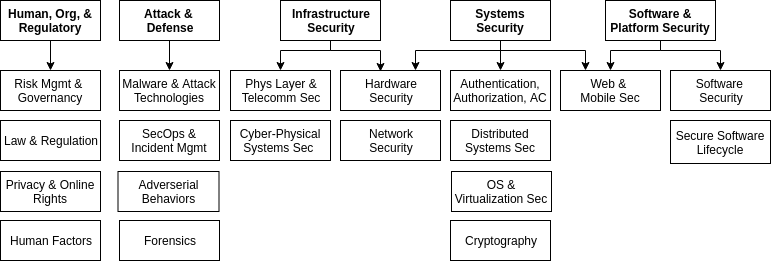
\includegraphics[width=.75\linewidth]{resource/img/ch_intro/taxonomies/cybok_vert_no_heading.png}
\caption{Cyber Security Body of Knowledge - Key Areas \cite{Rashid_Chivers_Danezis_Lupu_Martin}}
\label{fig:intro:cybok}
\end{figure} 


% \begin{figure}[ht]
% \centering
% 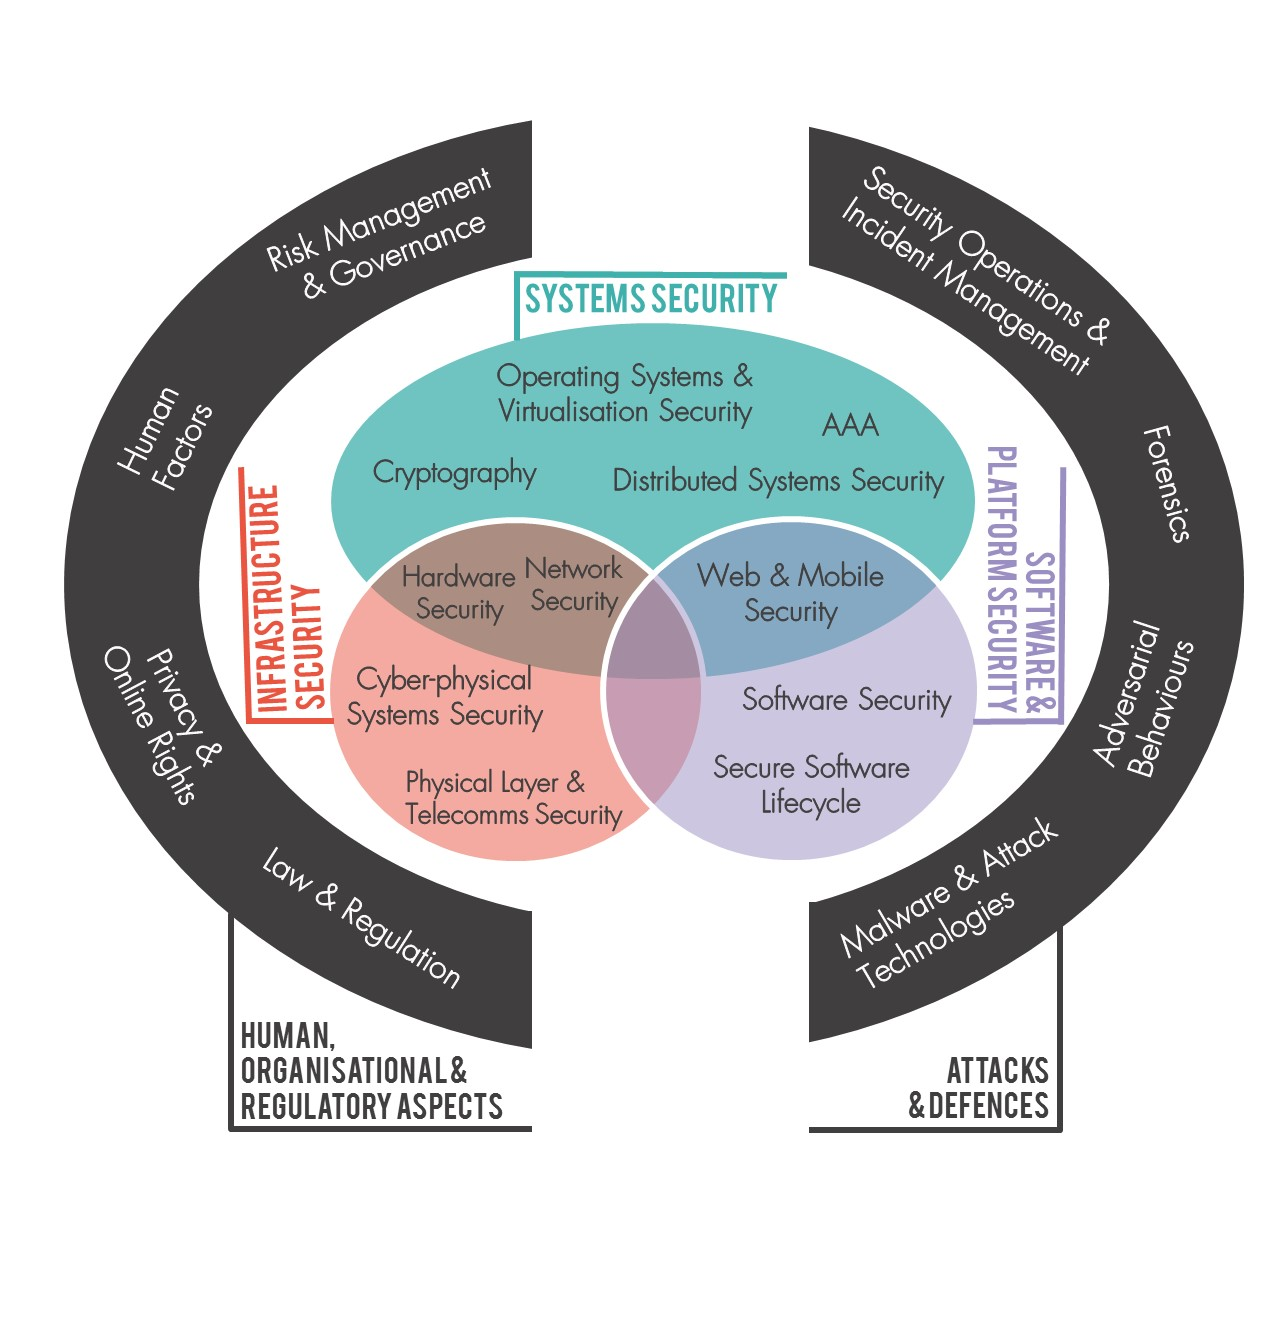
\includegraphics[width=.75\linewidth]{resource/img/ch_intro/CyBOK_clusters_-_Final.jpg}
% \caption{Cyber Security Body of Knowledge - Key Areas \cite{Rashid_Chivers_Danezis_Lupu_Martin}}
% \label{fig:intro:cybok}
% \end{figure} 

% Before discussing security metrics, we first take a step back to define what it is we intend to measure. 
Cyber security as a subject is at once broad and deep, covering a wide range of functional topics and skill sets. The lens through which a database administrator views security differs from that of a network engineer or an application developer within a particular business, and these perspectives may diverge from corresponding roles in other industry sectors. Thus, to effectively communicate any security objectives, it is necessary to understand the frame of reference from which they arise. In this work we refer to the Cyber Security Body of Knowledge\cite{Rashid_Chivers_Danezis_Lupu_Martin} (CyBoK) Key  Areas(KAs) as waypoints while navigating various aspects of security. The CyBoK project, sponsored by the UK's National Cyber Security Centre, provides both a taxonomy of cyber security topics, and a mapping to canonical references for these topics. Figure \ref{fig:intro:cybok} summarizes the 19 top level KAs and 5 broad categorical groupings.  Rather than delve into all the different CyBoK headings here in isolation, we elect instead to refer to the relevant classes as we encounter them in developing the thesis. 
%Finally, we provide working definitions for common terms found throughout this paper:

% Before discussing security metrics, we first take a step back to define what it is we intend to measure. 
% \begin{definition}
% \textbf{Metric}: The definition of a specific standard unit of measurement.
% \end{definition}
% \begin{definition}
% \textbf{Measurement}: A sampled value of a metric.
% \end{definition}
% \begin{definition}
% \textbf{Test}: The instrument and procedure used to obtain a measurement.
% \end{definition}
% \begin{definition}
% \textbf{Benchmark}: A standard environment and observed measurements for a metric.
% \end{definition}

Cyber security can be considered in terms of adversaries, along with their goals, and defenders, whose implicit goal is to prevent an adversary from achieving theirs. The purpose of a security metric is to quantify a specific aspect of cyber security, such as attacker
capabilities or defensive controls. We now frame the problem this work addresses by summarizing the security metrics and measurement techniques currently available, armed with the vocabulary and taxonomy needed to analyze them in context. 

\textbf{Regulatory and Compliance Metrics}: The left containing bracket in Figure \ref{fig:intro:cybok} depicts Human, Organizational, and Regulatory Aspects, and within the Risk Management KA\cite{Burnap_2019} we find the topic of security metrics. Indeed, security metrics are often defined within the scope of regulatory compliance. NIST's \textit{Security Metrics Guide for Information Technology Systems} \cite{Swanson_Bartol_Sabato_Hash_Graffo_2003,Chew_Swanson_Stine_Bartol_Brown_Robinson_2008}, ISO 27004 \textit{Monitoring, measurement, analysis and evaluation}\cite{iso_27004} and the Center for Internet Security's \textit{CIS Controls Measures \& Metrics}\cite{cis_cic} define the requirements for security metrics programs within various industry and government organisations. These security metrics are generally compliance focused, capturing statistics or percentages like employee training completion rate, number of hosts scanned and vulnerabilities found, or system performance complaints since the last patch roll out. 

\textbf{Operational Metrics} The right containing bracket in Figure \ref{fig:intro:cybok} labelled Attacks \& Defences includes security metrics listed in the \textit{Security Operations and Incident Response}\cite{Debar_2019} KA. The measurement processes in the operational area are distinguished primarily through automation support. Security Information and Event Management (SIEM) systems play a large role in collecting and aligning system telemetry for incident monitoring and response. SIEMs provide correlation of host/network event logs, IDS/IPS alerts, threat/vulnerability feeds, etc, and present a unified view of the system’s security posture automatically to the SOC. Before the advent of managed SIEMs, system administrators typically filled the role of security engineers, and relied on hand rolled collections of shell/perl scripts to manage systems, parse logs, collect or push events, format reports, and issue alarms.  To be effective required tribal knowledge along with proficiency in programming, network plumbing, and systems management, so changes to the environment or workforce made it extremely difficult(expensive) to deliver continuous monitoring capabilities to operators at any scale.  


\textbf{Vulnerability Metrics} Common to the 3 interior categories of Infrastructure, Systems, and Software \& Platform Security in Figure \ref{fig:intro:cybok} are vulnerability metrics. The Common Vulnerability Scoring System\cite{Mell07thecommon} (CVSS) is an open framework used throughout government and industry to report the severity of specific security vulnerabilities in commonly used software products. CVSS scores range from 0 to 10 based on the vulnerability’s exploitability and impact, with a score of 10 signifying the highest severity.  Exploitability is calculated by determining the access vector, access complexity, and number of authentication attempts required to exploit the vulnerability, with higher exploitability values equating to an easier compromise. Impact scores are determined by identifying the scope of a successful exploit on the vulnerable system’s confidentiality, integrity, and availability. 
%CVSS scores used in this research were queried using a local copy of the National Vulnerability Database (NVD) synchronized via MulVal's built-in mechanism and augmented with scores provided by vendors when an official Common Vulnerability Enumeration (CVE) designation was not available.  `


\begin{figure}[ht]
\centering
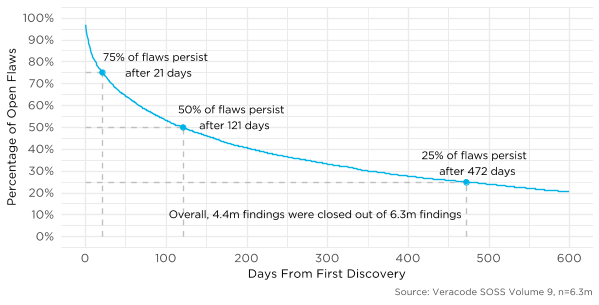
\includegraphics[width=.9\linewidth]{resource/img/ch_intro/veracode_closures_survival_analysis.png}
\caption{Veracode Static Analysis Remediation Times SOSS \cite{soss_v9}}
\label{fig:intro:soss-survival}
\end{figure} 


Static analysis\cite{Basili_Briand_Melo_1996} is a common method to identify possible vulnerabilities in software not included in the CVSS set. Developers can automatically scan custom source code and 3rd party libraries from within their IDE, or include hooks in their repository/CI to check incoming commits before merging. The metrics produced from static analysis can alert developers\cite{Johnson_2013} to common vulnerabilities in the code they write.  Figure \ref{fig:intro:soss-survival} shows the survival rate for static scan findings in 2018. 



\textbf{Economic Metrics} Measuring the trade-offs between competing interests and the incentives influencing actors is pervasive throughout cyber security. Security economics\cite{Anderson_2001} applies prevailing microeconomics models to describe limiting factors for attack and defense agents. The Gordon-Loeb\cite{Gordon_Loeb} model details an optimal security investment under the assumption of diminishing marginal returns.  In \textit{Security Metrics and Security Investment}\cite{Bohme_Moore} the authors derive metrics including the return on security investment (ROSI) and net present value (NPV) over future periods while accounting for different risk management temperaments. A survey of the economics of information security\cite{Anderson_Moore} literature summarizes potential applications of these economic metrics in many of the key cyber security areas. 


\begin{figure}[ht]
\centering
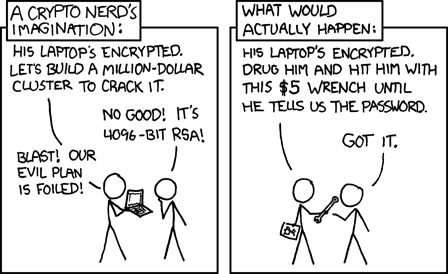
\includegraphics[width=.6\linewidth]{resource/img/ch_intro/xkcd_538_threat_model_econsec.png}
\caption{ source: https://www.xkcd.com/538/ }
\label{fig:intro:xkcd}
\end{figure} 

Figure \ref{fig:intro:xkcd} shows anecdotally one type of situation that economic metrics help us to avoid. Given an existing defensive capability that already deters attacks (data at rest cryptography in this case), further investment in that defense will give limited additional value. It also demonstrates the dangers of evaluating risk based on too narrow a security domain. Defining an attacker's capabilities, or threat modeling, is described in Section  \ref{sec:intro:threat_modeling}.


The evolution of information systems is trending away from a single administrative domain with a clear security boundary and moving towards a mix of self-hosted, provider managed, and remote 3rd party services. This creates unique challenges from an information security perspective, not least of which being how to define the new perimeter. 

% In order to evaluate the system's security posture in a mixed environment 

% while considering any architectural design changes made. Not only does this include a review of existing security controls, but also an assessment of the effects any regulatory compliance requirements will have on the deployment. Additionally, whereas a solution that resides totally in house can be evaluated in the context of a single security boundary, extending the perimeter to the public cloud requires an implicit acceptance that the cloud provider's administrative users have a higher privilege level than any tenant role that can be assigned. 

% A typical example being a company that maintains commercially sensitive data in house, but deploys access services to the public cloud and delegates authentication or authorization mechanics to vendors like Facebook or PayPal. 



\section{Automating Security Measurement} \label{sec:intro:devsecops}



\begin{figure}[ht]
\centering
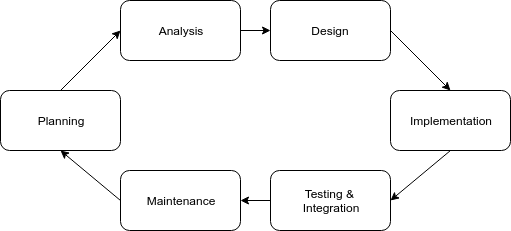
\includegraphics[width=.6\linewidth]{resource/img/ch_intro/sdlc.png}
\caption{Software Development Life Cycle}
\label{fig:intro:sdlc_redo}
\end{figure} 

% \begin{figure}[ht]
% \centering
% 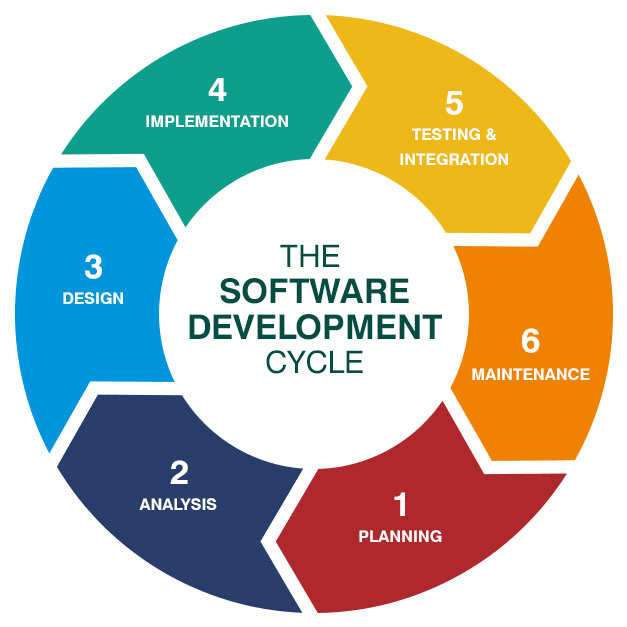
\includegraphics[width=.6\linewidth]{resource/img/ch_intro/sdlc_from_google.png}
% \caption{Software Development Life Cycle}
% \label{fig:intro:sdlc_redo}
% \end{figure} 

The software development life cycle shown in Figure \ref{fig:intro:sdlc_redo} is an iterative process that, until recently, was almost exclusively used within the Software \& Platform KA. Before the Agile\cite{Beck_2013} method was adopted, a single iteration of the SDLC could span several years, with planning, design, and analysis consuming a significant portion of the up front time and cost for the project. When a software project failed under this model, it happened because available funding was burned and often resulted in little or no working code. The Agile approach prefers faster iterations (often counted in weeks) with less emphasis on up front specifications. The result is a 'fail-fast' model that surfaces fundamental problems early and produces prototype software that may be salvaged and reused in other work if the project is abandoned. 

An ecosystem of tools exists around the SDLC that are mature, actively maintained, and most importantly (for us at least) almost entirely automated. Design requirements are captured in trackers that contain customizable metadata like priority, status, and dependencies. These requirements can link to code commits or PRs that satisfy the requirement, or customer created issues or development blockers that prevent the requirement from being closed. Unit, Integration, Regression, and Acceptance tests are run by continuous integration and delivery systems which can prevent breaking changes from entering the code base, roll back bad commits that do get merged, and deploy updates to production servers as dictated by the pipeline configuration. 

As an extension (and tacit endorsement) of the automated software CI/CD pipeline described above, development operations(DevOps) has recently emerged as the corollary in managing the life cycles components in the System and Infrastructure CyBOK categories. DevOps allows systems and network engineers to develop, test, deploy, and provision the supporting infrastructure required by an application in the same workflow, even from the same code base as the desired application. Maintaining the desired state of the underlying system in configuration files and provisioning scripts through a version control system is often called \textit{Infrastructure-as-Code}, While this is sometimes used to set up bare metal resources like servers and network appliances, the more common case currently is to provision infrastructure onto a self managed or commercial hypervisor using virtual machines or containerized micro services. 

\begin{figure}[ht]
\centering
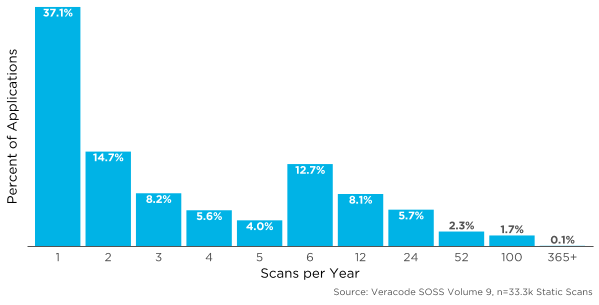
\includegraphics[width=.9\linewidth]{resource/img/ch_intro/veracode_scanfreq_percentages.png}
\caption{Veracode Freq Percentages SOSS \cite{soss_v9}}
\label{fig:intro:soss-scan-freq}
\end{figure} 

A functioning DevOps workflow integrates the application development and operations teams. The next logical step in this evolution is to disentangle the stovepiped security evaluation mechanisms built around each of these formerly independent areas. The resulting field of SecDevOps (or DevSecOps\cite{Rahman_Williams_2016}) is \textit{not} the sum of the security of each part (although it will likely be treated that way at least until the community converges on which term to reference it by). Rather, it should trigger a re-assessment of previous security controls and best practices prescribed through existing regulatory and compliance frameworks. 

For example, Figure \ref{fig:intro:soss-scan-freq} shows the yearly count from over 33 thousand source code scans in 2018 as reported by Veracode. While this data is from a single vendor, the results are still concerning. The median number of security scans per year was just 2. We presume there is regulatory or compliance pressure to scan at least once per year. Given the percentage of applications that scan once a week or more is just over 4\%, we can also infer that most customers either don't have an automated development workflow in house, or if they do have chosen not to integrate this capability. 


\begin{figure}[ht]
\centering
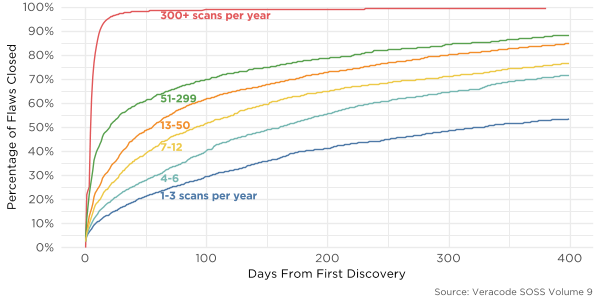
\includegraphics[width=.9\linewidth]{resource/img/ch_intro/veracode_scanfreq_vs_closures.png}
\caption{Veracode Scan Frequencies vs Closures SOSS \cite{soss_v9}}
\label{fig:intro:soss-scan-freq-closures}
\end{figure} 

While we can't extrapolate with confidence the closure rates in Figure \ref{fig:intro:soss-survival} to CVSS findings, or the scan rates in Figure \ref{fig:intro:soss-scan-freq} to users of alternative static analysis products, we can draw a very clear line between the teams that scan their code as part of an automated development workflow and their ability to address security findings. Figure \ref{fig:intro:soss-scan-freq-closures} displays a distinct stratification of response times based on scan frequency. Indeed, the teams that incorporated a simple static analysis check into their DevOps pipeline were able to remediate nearly all found flaws before the others could fix half. What we observed from Figure \ref{fig:intro:soss-survival}, that around half the observed samples only conducted one or two scans per year suggests that, in this context, they were only able to fix about 50\% of the identified flaws after more than 400 days. Referring back to the Agile development principals that DevOps workflows are based upon, we can surmise the relative speed in addressing flaws is attributable to small incremental changes with actionable feedback after each change. 




% The motivation of this thesis is to make modern information systems more secure, and the driving force behind that goal is automation. Many of the problems addressed in this work stem from the disparate ecosystem of tools, APIs, methodologies, libraries, and frameworks that exist in relative isolation to one another. 

% Consider Security Information and Event Management (SIEM) systems as an example, which provide correlation of host/network event logs, IDS/IPS alerts, threat/vulnerability feeds, etc, and present a unified view of the system’s security posture automatically to the SOC. Before the advent of managed SIEMs, sys admins typically filled the role of security engineers, and relied on hand rolled collections of shell/perl scripts to manage systems, parse logs, collect or push events, format reports, and issue alarms. To be effective required tribal knowledge along with proficiency in programming, network plumbing, and systems management, so changes to the environment or workforce made it extremely difficult(expensive) to deliver continuous monitoring capabilities to operators at any scale. 
% We are in a similar state today with network design and enterprise planning. Infrastructure-as-Code, SDN, virtualization and containerization are all critical components in modern deployments, but the glue that ties them together is largely ad-hoc, and risk evaluation is still a manual task. 




% In order to understand the security posture before a system is rolled out and SIEMs are in place, we are creating a tool to facilitate the automated analysis, collection, correlation, and dissemination of the security metrics mentioned above. The necessity of such a tool is critical to evaluating the efficacy of the metrics reviewed above, and provides the foundation for ongoing research in machine learning models for secure systems planning, design, and evolution.




% \textbf{Software Security Metrics} 



\section{Contributions}\label{sec:intro:contibutions}

% contribuutions



% \begin{figure}[tbph]
% \centering
% 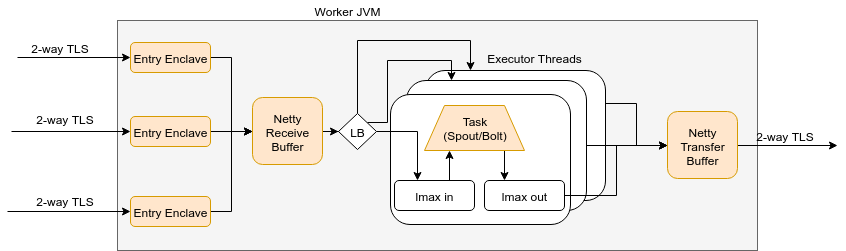
\includegraphics[width=.5\linewidth]{resource/img/ch_intro/stormsgx.png} %Include graphic at 1=100 \% linewidth vs textwidth as it will size if put in columns. Textwidth wont resize in columns
% \caption{Storm SGX architecture}
% \label{fig:sgx_arch}
% \end{figure} 

% In this thesis we provide a framework for the systematic validation of the existing security metrics body of knowledge. In doing so we endeavour not only to survey the current state of the art, but also to create a common platform for future research in the area to be conducted. 

% We  then  demonstrate  the  utility  of  our  framework  through  the  evaluation  of  leading security metrics against a reference set of system models we have created.  

% We investigate how  to  calibrate  security  metrics  for  different  use  cases  and  establish  a new methodology  for security metric benchmarking. To support automated and repeatable testing, each metric is implemented as an independent module containing the computation logic. These metric implementations can then be called directly from an embedded library, accessed through a benchmark test with standard interfaces and return types, or managed with a container orchestration engine. Each test has an associated specification which is used to configure dependencies and tuning parameters for execution. 
% Specifically, we:
% \begin{itemize}
% \item Provide a methodology for calibrating security metrics against a fixed baseline and demonstrate isolation criteria for benchmark regimens
% \item  Implement several distinct execution paradigms for different use cases 
% \item Describe validation mechanisms available through increasingly sophisticated modeling and simulation extensions
% \end{itemize}

% We further explore the research avenues unlocked by automation through our concept of an API driven S-MaaS (Security Metrics-as-a-Service) offering. We review our design considerations in packaging security metrics for programmatic access, and discuss how various client access-patterns are anticipated in our implementation strategy. Using existing metric processing pipelines as reference, we show how the simple, modular interfaces in S-MaaS support dynamic composition and orchestration. We anticipate consumers will fall into one or more of the following access patterns:
% \begin{itemize}
% \item \textbf{R\&D}: A clean environment for developing and testing metrics.
% \item \textbf{Reporting}: Measurements are pushed to persistent storage or pulled from a client into a structured format for charting and analysis. 
% \item \textbf{Batch}: Client asynchronously submits a collection of inputs to calculate metrics for, with the target use-case being dataset preparation for supervised learning.
% \item \textbf{Stream}: Client defines dependency graphs amongst metrics and connects these topologies to data sources for continuous stream processing.  
% \end{itemize}


% To summarize:
% \begin{itemize}
% \item We created a rapid prototyping and integration environment for security metrics. 
% \item We developed a reference data set for validating security metrics across different topologies and scales.
% \item We implemented benchmark tests in a widely adopted open source benchmark test suite to reach the largest audience. 
% \item We developed S-MaaS, a scalable deployment system where metrics are microservices.
% \item We enhanced S-MaaS automation using a variety of machine learning applications.
% \item We present case studies and lessons learned as evidence our framework is practical and effective.

% \end{itemize}






 %\label{ch:intro}

\chapter{Background} \label{ch:background}


Aristotle is often credited with founding the fields of natural science in the West; with the story going that he disagreed with his teacher Plato on the matter of philosophical thought, arguing that it should be based on observations from the natural world. We consider observations to be  \textit{measurements} when they are quantified with respect to an agreed upon scale, or measurement unit. The first measurement units were used in bartering to standardize the exchange values of different commodities\cite{Morris_2001}. To measure length, for example, the torso was consistent enough across people to be considered a measurement unit, from which other units like the hand, the foot, and the cubit were derived. A \textit{quantity} refers specifically to a property that can be measured, in this case length. Although the term is often\cite{Debievre_2009} overloaded to mean the amount of something as well, we attempt to be metrologically consistent in this work by referring to the property to be measured as the quantity or \textit{measurand}, and the \textit{amount} of some thing as the observed value in terms of magnitude and measurement unit. 

In recent years effort has been spent investigating the science of cyber security\cite{Kott_2014, Schneider, Chang_2019, Spring_Moore_Pym_2017}. In the \textit{NSF/IARPA/NSA Workshop on the Science of Security}\cite{Evans_2008} three directions of research were identified to improve the scientific foundations of security, \textit{metrics}, \textit{formal methods}, and \textit{experimentation}. In this thesis we focus particularly on the role of metrics in security research, although well-defined system models and experimentation environments both play key roles in the analysis. In this chapter we review the relevant concepts in security metrics needed to build our framework. Section \ref{sec:background:modeling} describes methods for representing different components influencing security. These models are the inputs to the security property being measured, and in Section \ref{sec:background:metrics} we describe the types of metrics available and how they relate. %In section \ref{sec:background:metric_validation} we describe techniques used to ensure the instruments used to measure security are accurate and consistent. 



\section{Security Modeling}\label{sec:background:modeling}

\input{content/chapters/ch_background/sec_modeling/modeling_intro.tex}

\subsection{Infrastructure \& System Modeling}

\input{content/chapters/ch_background/sec_modeling/infrastructure}\label{sec:background:modeling:infra_modeling}

\subsection{Threat Modeling}

\input{content/chapters/ch_background/sec_modeling/attack_modeling.tex}\label{sec:background:modeling:attack_modeling}


\subsection{Graph Based Models}\label{sec:background:modeling:attack_graphs}

\input{content/chapters/ch_background/sec_modeling/attack_graphs.tex}

\subsection{Summary}\label{sec:background:modeling:summary}

\input{content/chapters/ch_background/sec_modeling/summary.tex}

% \section{Terminology}\label{sec:background:terminology}

% \section{Security Modeling}\label{sec:background:modeling}

% 
An argument can be made that the accuracy of any measurement taken from a model is limited, and that the only true test of security is in measuring the production system. While it is possible to test systems in production, these tests can be disruptive to operations, for example when testing fire alarms in a building or conducting social engineering on customers or staff. We can recreate the production system on a cyber range\cite{Yamin_Katt_Gkioulos_2020} or similar dedicated environment for security testing, without the advantages of or impact on live traffic. In many cases we can interrogate the production system for values from which to build a model, but only if the system is in production. Design time tools are abundant throughout the CyBOK KAs, but the backend models used by tools differs in schema and accessibility, making integration with security metrics difficult. The role models play varies widely depending on the area of cyber security, with intrusion detection and antivirus systems on one end of the spectrum requiring production traffic for testing and evaluation, and cryptographic protocols on the other end having model based proofs of their security properties (although implementation is a different matter). The regulatory and compliance frameworks listed in Section \ref{sec:intro:threat_modeling} are made up of individual security controls, each of which can fall somewhere on this empirical spectrum. The use of models may be overly naive for some cases, but where applicable, models enable programmatic access and rapid prototyping, and allow us to isolate specific security properties for measurement through simulation and analysis at a speed not possible with live systems. In the rest of this section we provide some useful models that we make use of in later chapters. 

% \subsection{Infrastructure \& System Modeling}

% 

\section{Security Modeling}\label{sec:background:modeling}

\input{content/chapters/ch_background/sec_modeling/modeling_intro.tex}

\subsection{Infrastructure \& System Modeling}

\input{content/chapters/ch_background/sec_modeling/infrastructure}\label{sec:background:modeling:infra_modeling}

\subsection{Threat Modeling}

\input{content/chapters/ch_background/sec_modeling/attack_modeling.tex}\label{sec:background:modeling:attack_modeling}


\subsection{Graph Based Models}\label{sec:background:modeling:attack_graphs}

\input{content/chapters/ch_background/sec_modeling/attack_graphs.tex}

\subsection{Summary}\label{sec:background:modeling:summary}

\input{content/chapters/ch_background/sec_modeling/summary.tex}\label{sec:background:modeling_main}

% 
%  MulVal\cite{Ou_Appel_2005} provides an efficient\cite{Rao_1997} Datalog based modeling language and inference engine for vulnerability relationship analysis. The input model consists of configurations for \textbf{hosts} and \textbf{networks}, \textbf{principals} describing user accounts and privileges, rules governing \textbf{interactions}, and access \textbf{policies}. Information about the system under test is either gathered through standard methods such as Nessus, Nmap, and OVAL scans or defined manually for hypothetical data points, and parsed into the global system model using an appropriate adaptor. MulVal can then make inferences about how the entities are able to interact. When provided with a starting and ending node, MulVal enumerates all possible paths an attacker may traverse to compromise the target. The attack graph represents the exploitable vulnerabilities in a system as the set of connected nodes and edges between an attacker’s origin and the target.
 


% \cite{Chowdhary_Pisharody_Huang_2016} Provides a moving target defense solution 

The OSI 7-layer model\cite{Zimmermann_1980} describes network communication as a stack of protocols built on top of a \textit{Physical} transport medium such as copper, optical fiber, or radio. On top of the physical layer are the Layer 2 \textit{Data Link} protocols that facilitate reading and writing frames to and from the given physical circuit including source and destination addressing (\textit{Medium Access Control}), and the protocols that encapsulate/de-encapsulate upper layer packets into the frame format suitable for transmission across the medium (\textit{Logical Link Control}). When a datagram from the upper layers is transmitted to a remote system, it is encapsulated into one or more packets at the \textit{Network} layer, the packets are then encapsulated into frames at the Data Link Layer, and the frames are placed onto the physical medium.  When a frame is received at the destination, it is de-encapsulated and the payload is handed up to the Layer 3 \textit{Network} protocol capable of processing the packet. Encapsulation or de-encapsulation occurs between each layer in the OSI model and  adds processing overhead and increased latency to traffic. Layer 2 traffic is not routable, since routing information like IP address is stored in the Layer 3 header. 

% [width=90mm]
\begin{figure}[ht]
\centering
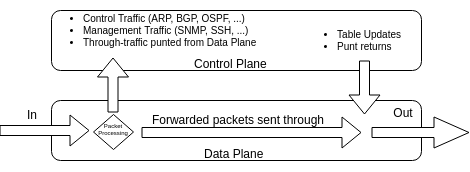
\includegraphics[width=.8\linewidth]{resource/img/ch_background/sdn_analytics/router_flow_2.png}
\caption{Traffic flow between planes}
\label{fig:router_flow}
\end{figure} 
Network device traffic can be partitioned into two planes\cite{Khosravi_Anderson_2003}: the \textit{Forwarding (or Data) Plane} consists of traffic passing through the device while \textit{Control Plane} traffic has the network element as its destination. We consider the \textit{Management Plane} a subset of the \textit{Control Plane}. Forwarding plane components do the heavy lifting in a network device by connecting incoming traffic to the appropriate outgoing port. When the forwarding element can't identify the correct egress port the packet is sent up to the control plane for a routing solution as shown in Figure \ref{fig:router_flow}. The control plane can request and process information about link status and network topology from peers and update forwarding tables in the data plane in response. 

In conventional network equipment the control and data planes are tightly coupled. That is, the components responsible for forwarding packets are physically located along side the components used to make routing and switching decisions about that traffic. How these systems are laid out in practice varies widely by function and vendor. Figure \ref{fig:router_conventional} depicts a notional router. Line cards house the forwarding engine in Application Specific Integrated Circuits (ASICs), Network Processing Units (NPUs), or even software deployed on virtual machines. Incoming traffic is read off the port into a buffer, the packet header is examined to query the Forwarding Information Base for the destination, the packet processor alters the header as needed, and the packet is forwarded out the appropriate egress port. If the traffic is destined for the device (that is, control or management plane) or if the FIB lookup failed, the packets are queued in the receive path buffer for transfer to the routing engine. The routing engine is typically housed on another line card and connected to the forwarding modules through the backplane or switch fabric. Control plane services are hosted by the network OS running on commodity CPUs. The primary purpose of the control plane service suite is to manipulate the forwarding plane lookup tables based on routing and signalling information it receives. It maintains the Routing Information Base (RIB) used to optimize local FIBs and provides the interface for router management and configuration. 

\begin{figure}[h]
\begin{tabular}{p{0.48\textwidth}p{0.48\textwidth}}
\begin{minipage}{.48\textwidth}
\centering
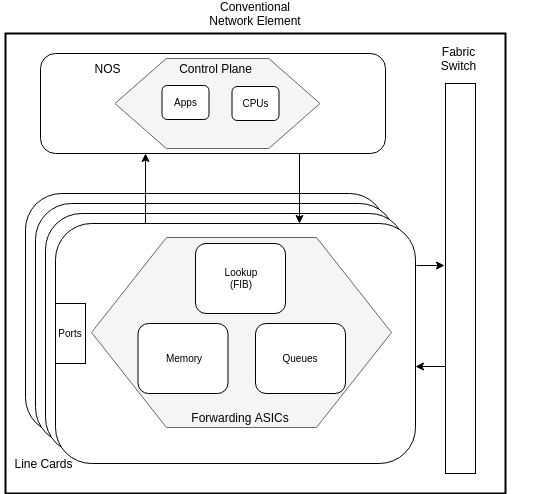
\includegraphics[width=.9\linewidth]{resource/img/ch_background/haec/sgx/sdn/router_conventional.png}
\caption{Conventional Element}
\label{fig:router_conventional}
%\end{figure} 
\end{minipage}
&
\begin{minipage}{.47\textwidth}
\centering
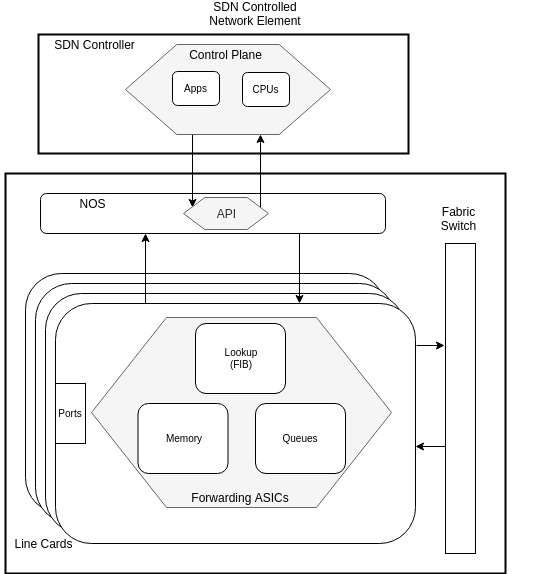
\includegraphics[width=.9\linewidth]{resource/img/ch_background/sdn_analytics/router_sdn.png}
\caption{SDN Controlled Element}
\label{fig:router_sdn}
\end{minipage}
\end{tabular}
\end{figure}

SDN systems decouple the forwarding and control plane elements further, by centralizing controller functionality outside the data plane's enclosure and introducing a southbound interface with which to alter forwarding tables via API. This allows SDN controllers to scale independently of the forwarding elements and receive state information for all network devices it oversees. Since the complex decision logic has been extracted from the forwarding units, the core elements in SDN are simple switches. The result is a control plane that can optimize the forwarding rules it pushes based on global requirements instead of the limited view available to conventional devices. This also results in a potentially larger attack surface and single point of failure. 

Carrier network architectures can be decomposed into tiers based on functionality and proximity to the end users. The \textit{Access} tier is the forward facing attachment point for a user such as the radio tower a mobile device connects with or the set top box that joins a home network to the ISP. The \textit{Provider Edge } provides the services needed to manage traffic between the various access platforms and the provider core. One or more \textit{Aggregation} layers can be added to consolidate provider edge points based on access density requirements. Finally, the \textit{Provider Core} provides hi speed transit between edge nodes. 

% $<$ carrier network diagram here? $>$

% \subsection{Existing Model}\label{subsec:existing_model}
% \input{content/contrib/inrfa/infra_model.tex}

% \subsection{Layer 2}\label{subsec:infra_l2}
% \input{content/contrib/inrfa/layer2.tex}
% \subsection{Layer 3}\label{subsec:infra_l3}
% \input{content/contrib/inrfa/layer3.tex}


% \begin{figure}[H]
% \begin{tabular}{p{0.5\textwidth}p{0.5\textwidth}}
% \begin{minipage}{.5\textwidth}
% \begin{lstlisting}[style=datalog, label={lst:preds}, caption={preds.P \cite{Ou_Boyer_McQueen_2006}}]

% /******************************************************/
% /****         Predicates Declaration              *****/
% /******************************************************/

% primitive(inCompetent(_principal)).
% primitive(competent(_principal)).
% primitive(clientProgram(_host, _programname)).
% primitive(vulExists(_host, _vulID, _program)).
% primitive(vulProperty(_vulID, _range, _consequence)).
% primitive(hacl(_src, _dst, _prot, _port)).
% primitive(attackerLocated(_host)).
% primitive(hasAccount(_principal, _host, _account)).
% primitive(networkServiceInfo(_host, _program, _protocol, _port, _user)).
% primitive(setuidProgramInfo(_host, _program, _owner)).
% primitive(nfsExportInfo(_server, _path, _access, _client)).
% primitive(nfsMounted(_client, _clientpath, _server, _serverpath, _access)).
% primitive(localFileProtection(_host, _user, _access, _path)).
% primitive(dependsOn(_h, _program, _library)).
% primitive(installed(_h, _program)).
% primitive(bugHyp(_,_,_,_)).
% primitive(vulExists(_machine,_vulID,_program,_range,_consequence)).
% primitive(canAccessFile(_host, _user, _access, _path)).
% primitive(isWebServer(_host)).
% meta(cvss(_vulID, _ac)).


% derived(execCode(_host, _user)).
% derived(netAccess(_machine,_protocol,_port)).
% derived(canAccessHost(_host)).
% derived(accessFile(_machine,_access,_filepath)).
% derived(accessMaliciousInput(_host, _principal, _program)).
% derived(principalCompromised(_victim)).
% derived(dos(_host)).
% derived(logInService(_host, _protocol, _port)).

% meta(attackGoal(_)).
% meta(advances(_, _)).

% /******************************************************/
% /****         Tabling Predicates                  *****/
% /*   All derived predicates should be tabled          */
% /******************************************************/

% :- table execCode/2.
% :- table netAccess/3.
% :- table canAccessHost/1.
% :- table canAccessFile/4.
% :- table accessFile/3.
% :- table principalCompromised/1.
% :- table vulExists/5.
% :- table logInService/3.
% \end{lstlisting}
% \label{fig:eg_net01}
% %\end{figure} 
% \end{minipage}
% &
% \begin{minipage}{.5\textwidth}
% % \begin{adjustbox}{width=\textwidth}
% \begin{lstlisting}[style=datalog, label={lst:rules}, caption={input.P \cite{Ou_Boyer_McQueen_2006}}]

% /******************************************************/
% /****         Interaction Rules                   *****/
% /******************************************************/

% /****** Section execCode ******
% interaction_rule(
%   (execCode(H, Perm) :-
% 	hasAccount(P, H, Perm)),
%   rule_desc('Insider threat', 1)).
% */

% interaction_rule(
%   (execCode(Host, Perm) :-
% 	principalCompromised(Victim),
% 	hasAccount(Victim, Host, Perm),
% 	canAccessHost(Host)),
%   rule_desc('When a principal is compromised any machine he has an account on will also be compromised',
%   0.5)).

% interaction_rule(
%   (execCode(Host, root) :-
% 	execCode(Host, _Perm2),
% 	vulExists(Host, _, Software, localExploit, privEscalation)),
%   rule_desc('local exploit',
%   1.0)).

% interaction_rule(
%   (execCode(H, Perm) :-
% 	vulExists(H, _, Software, remoteExploit, privEscalation),
% 	networkServiceInfo(H, Software, Protocol, Port, Perm),
% 	netAccess(H, Protocol, Port)),
%   rule_desc('remote exploit of a server program',
%   1.0)).

% interaction_rule(
%   (execCode(H, Perm) :-
%         vulExists(H, _, Software, remoteClient, privEscalation),
% 	hasAccount(Victim, H, Perm),
%         accessMaliciousInput(H, Victim, Software)),
%   rule_desc('remote exploit for a client program',
%   0.5)).

% interaction_rule(
%   (execCode(H, root) :-
% 	accessFile(H, write, _Path)),
%   rule_desc('Trojan horse installation',
%   0.8)).

% /* Singleton variable at head
% interaction_rule(
%  (execCode( Attacker, Host, _) :-
%   execCode(Attacker, Host, root)),
%   'execution at any level if root execution').
% */

% \end{lstlisting}
% % \end{adjustbox}
% \end{minipage}
% \end{tabular}
% \end{figure}




% \begin{figure}[H]
% \begin{tabular}{p{0.5\textwidth}p{0.5\textwidth}}
% \begin{minipage}{.5\textwidth}
% \begin{lstlisting}[style=datalog, label={lst:preds}2, caption={preds.P \cite{Ou_Boyer_McQueen_2006}}]


% /******** Section netAccess ********/
% /* accessing a host through network according to a hacl policy.
%   For now we assume that every user on a local
%   machine has access to network. this may change
%   later. */
% interaction_rule(
%   (netAccess(H2, Protocol, Port) :-
% 	execCode(H1, _Perm),  /* Any permission level */
% 	advances(H1, H2),
%     hacl(H1, H2, Protocol, Port)),
%   rule_desc('multi-hop access',
%   0.5)).

% interaction_rule(
%   (netAccess(H, Protocol, Port) :-
% 	attackerLocated(Zone),
% 	hacl(Zone, H, Protocol, Port)),
%   rule_desc('direct network access',
%   1.0)).

% interaction_rule(
%   (netAccess(H, Protocol, Port) :-
% 	attackerLocated(H)),
%   rule_desc('direct on-host access',
%   1.0)).



% /****** Section canAccessHost ******/
% interaction_rule(
%   (canAccessHost(H) :-
% 	execCode(H, _Perm)),
%   rule_desc('Access a host through executing code on the machine',
%   1.0)).

% interaction_rule(
%   (canAccessHost(H) :-
% 	logInService(H, Protocol, Port),
% 	netAccess(H, Protocol, Port)),
%   rule_desc('Access a host through a log-in service',
%   1.0)).


% /******** Section accessFile ********/
% interaction_rule(
%   (accessFile(H, Access, Path) :-
% 	execCode(H, Usr),
% 	canAccessFile(H, Usr, Access, Path)),
%   rule_desc('execCode implies file access',
%   1.0)).


% /****** Section principalCompromised ******/
% interaction_rule(
%   (principalCompromised(Victim) :-
% 	hasAccount(Victim, H, _Perm),
% 	execCode(H, root)),
%   rule_desc('password sniffing',
%   0.8)).

% interaction_rule(
%   (principalCompromised(Victim) :-
% 	hasAccount(Victim, H, User),
% 	execCode(H, User)),
%   rule_desc('password sniffing',
%   0.8)).



% \end{lstlisting}
% \label{fig:eg_net01}
% %\end{figure} 
% \end{minipage}
% &
% \begin{minipage}{.5\textwidth}
% % \begin{adjustbox}{width=\textwidth}
% \begin{lstlisting}[style=datalog, label={lst:preds4}, caption={input.P \cite{Ou_Boyer_McQueen_2006}}]

% /*
% interaction_rule(
%   (principalCompromised(Victim) :-
% 	inCompetent(Victim)),
%   rule_desc('incompetent user',
%   0.2)).
% */

% /********************************************************/
% /*      Software specific knowledge                     */
% /********************************************************/

% /*
% explain(logInService(H, Protocol, Port), Text) :-
% 	fmt_write_string(Text,
%   "There is a login service running under protocol %S and port %S on host %S.", args(Protocol, Port, H)).
% */



% /***************** Section ssh **********************/
% interaction_rule(
%   (logInService(H, Protocol, Port) :-
% 	networkServiceInfo(H, sshd, Protocol, Port, _)),
%   rule_desc('',
%   1)).

% interaction_rule(
%   (logInService(H, Protocol, Port) :-
% 	networkServiceInfo(H, vpnService, Protocol, Port, _)),
%   rule_desc('',
%   1)).


% /**************** Section  nfs *****************/
% /* Principal P can access files on a NFS server if the files
%   on the server are mounted at a client and he can access the
%   files on the client side */
% interaction_rule(
%   (accessFile(Server, Access, ServerPath) :-
% 	nfsMounted(Client, ClientPath, Server, ServerPath, Access),
% 	accessFile(Client, Access, ClientPath)),
%   rule_desc('NFS semantics',
%   1)).


% /* Principal P can access files on a NFS client if the files
%   on the server are mounted at the client and he can access the
%   files on the server side */
% interaction_rule(
%   (accessFile(Client, Access, ClientPath) :-
% 	nfsMounted(Client, ClientPath, Server, ServerPath, read),
% 	accessFile(Server, Access, ServerPath)),
%   rule_desc('NFS semantics',
%   1)).


% interaction_rule(
%   (accessFile(Server, Access, Path) :-
% 	execCode(Client, _User),
%     nfsExportInfo(Server, Path, Access, Client),
%     hacl(Client, Server, nfsProtocol, nfsPort)),
%   rule_desc('NFS shell',
%   0.8)).
% \end{lstlisting}
% % \end{adjustbox}
% \end{minipage}
% \end{tabular}
% \end{figure}



% \begin{figure}[H]
% \begin{tabular}{p{0.5\textwidth}p{0.5\textwidth}}
% \begin{minipage}{.5\textwidth}
% \begin{lstlisting}[style=datalog, label={lst:preds5}, caption={preds.P \cite{Ou_Boyer_McQueen_2006}}]



% interaction_rule(
%   (canAccessFile(H, Usr, Acc, Path) :-
% 	localFileProtection(H, Usr, Acc, Path)),
%   rule_desc('',
%   1)).

% /* Singleton variable in head
% interaction_rule(
%   (canAccessFile(_H, root, _Access, _Path)),
%   'root has arbitrary access').
% */



% interaction_rule((vulExists(H, ID, Sw, Range, Consequence):-
% 	        vulExists(H, ID, Sw),
% 		vulProperty(ID, Range, Consequence)),
%              rule_desc('',
%              1)).

% interaction_rule((vulExists(H, _ID, Sw, Range, Consequence):-
% 	        bugHyp(H, Sw, Range, Consequence)),
%              rule_desc('Introducing hypothetical bug',
%              1)).


% interaction_rule((vulExists(H, ID, Sw, Range, Consequence):-
% 	        vulExists(H, ID, Library, Range, Consequence),
% 		dependsOn(H, Sw, Library)),
%              rule_desc('Library bug',
%              1)).

% interaction_rule(
%   (accessMaliciousInput(H, Victim, Software) :-
%      inCompetent(Victim),
%      hacl(H, MaliciousMachine, httpProtocol, httpPort),
%      attackerLocated(MaliciousMachine)),
%   rule_desc('Browsing a malicious website', 0.8)).

% interaction_rule(
%   (accessMaliciousInput(H, Victim, Software) :-
%      competent(Victim),
%      hacl(H, MaliciousMachine, httpProtocol, httpPort),
%      attackerLocated(MaliciousMachine)),
%   rule_desc('Browsing a malicious website', 0.1)).


% \end{lstlisting}
% \label{fig:eg_net01}
% %\end{figure} 
% \end{minipage}
% &
% \begin{minipage}{.5\textwidth}
% % \begin{adjustbox}{width=\textwidth}
% \begin{lstlisting}[style=datalog, label={lst:preds6}, caption={input.P \cite{Ou_Boyer_McQueen_2006}}]


% interaction_rule(
%   (accessMaliciousInput(H, Victim, Software) :-
%      inCompetent(Victim),
%      isWebServer(CompromisedMachine),
%      hacl(H, CompromisedMachine, httpProtocol, httpPort),
%      execCode(CompromisedMachine, _)),
%   rule_desc('Browsing a compromised website', 0.4)).


% /*
% interaction_rule(
%   (canAccessMaliciousInput(H, Browser) :-
%      installed(H, Browser),
%      isWebBrowser(Browser)),
%   rule_desc('A browser can potentially access malicious input',
%   1)).


% interaction_rule(
%   (canAccessMaliciousInput(H, Software) :-
% 	vulExists(H, _, Software, remoteClient, privEscalation),
% 	inCompetent(Victim),
% 	hasAccount(Victim, H, _Perm)),
%   rule_desc('A remote client vulnerability can potentially access malicious input from a host used by careless user',
%   1)).



% interaction_rule(
%   (canAccessMaliciousInput(H, Browser) :-
%      installed(H, Browser),
%      isWebBrowser(Browser),
%      hacl(H, MaliciousMachine, httpProtocol, httpPort),
%      attackerLocated(MaliciousMachine)),
%   rule_desc('Browsing a malicious website',
%   1)).

% interaction_rule(
%   (canAccessMaliciousInput(H, Browser) :-
%      installed(H, Browser),
%      isWebBrowser(Browser),
%      hacl(H, CompromisedMachine, httpProtocol, httpPort),
%      execCode(CompromisedMachine, _)),
%   rule_desc('Browsing a compromised website',
%   0.4)).

% interaction_rule(
%   (canAccessMaliciousInput(H, EmailClientSoftware) :-
%      installed(H, EmailClientSoftware),
%      isEmailClient(EmailClientSoftware),
%      isEmailServer(EmailServerSoftware),
%      hacl(H, EmailServer, EmailProtocol, EmailPort),
%      networkServiceInfo(EmailServer, EmailServerSoftware,
%                                 EmailProtocol, EmailPort, _Perm)),
%   rule_desc('receive an email message',
%   0.4)).

% \end{lstlisting}
% % \end{adjustbox}
% \end{minipage}
% \end{tabular}
% \end{figure}




% \begin{figure}[H]
% \begin{tabular}{p{0.5\textwidth}p{0.5\textwidth}}
% \begin{minipage}{.5\textwidth}
% \begin{lstlisting}[style=datalog, label={lst:tr_rules1}, caption={iav.P \cite{Ou_Boyer_McQueen_2006}}]


% /*
% IAV Network State Model
% */


% /*
%   attacker is at the customer edge or internet 
%   pe1 is CRS with vuln CVE-2012-1342 (BGP overflow remote code execution)
%   target is core router p3 control plane code execution

% _c control plane interface
% _d data plane interface
% _m management interface
% */
% attackerLocated(ce1).
% attackGoal(execCode(p3_c, _)).

% /*
% Customer Edge devices attach to Provider Edges
% control plane to exchange routing tables/VRFs
% through BGP
% */
% /* BGP b/t customer and provider edge */
% /* update 20160425: data and control from customer on same PE port */
% /*hacl(ce1, pe1_c,  tcp, 179).*/
% hacl(ce1, pe1_d,  _, _). 
% hacl(pe1_d, pe1_c,  _, _).

% /* 
% Customer data flows through PE data plane on predefined label switched path (MPLS tunnel)
% */

% /*
% Provider Edge devices talk to other PEs
% BGP b/t provider edges control plane to
% exchange client VRFs for tunnel endpoints 
% */
% hacl(pe1_c, pe2_c,  TCP, 179).
% hacl(pe1_c, pe4_c, TCP, 179).
% hacl(pe2_c, pe3_c, TCP, 179).
% hacl(pe2_c, pe1_c, TCP, 179).
% hacl(pe3_c, pe4_c,  TCP, 179).
% hacl(pe3_c, pe2_c,  TCP, 179).
% hacl(pe4_c, pe1_c,  TCP, 179).
% /*hacl(pe4_c, pe3_c,  TCP, 179). handle Cycles*/

% /*
% PEs also talk to neighbor P nodes over LDP 
% */
% hacl(pe1_c, p1_c,  TCP, 646).
% hacl(pe2_c, p1_c, TCP, 646).
% hacl(pe3_c, p3_c,  TCP, 646).
% hacl(pe4_c, p3_c,  TCP, 646).

% \end{lstlisting}
% \label{fig:eg_net01}
% %\end{figure} 
% \end{minipage}
% &
% \begin{minipage}{.5\textwidth}
% % \begin{adjustbox}{width=\textwidth}
% \begin{lstlisting}[style=datalog, label={lst:tr_rules2}, caption={input.P \cite{Ou_Boyer_McQueen_2006}}]

% /* 
% allow PEs to speak BGP with Aggregation P's 
% (this is to give us an attack path on the control plane, 
% other wise no path would exist)
%  */
% hacl(pe1_c, p1_c,  TCP, 179).
% hacl(pe2_c, p1_c, TCP, 179).
% hacl(pe3_c, p3_c, TCP, 179).
% hacl(pe4_c, p3_c,  TCP, 179).
% /* 
% hacl(pe1_c, p1_c,  TCP, 179).
% hacl(pe2_c, p1_c, TCP, 179).
% hacl(p1_c, pe1_c,  TCP, 179).
% hacl(p1_c, pe1_c, TCP, 179).
% hacl(p3_c, pe3_c, TCP, 179).
% hacl(p3_c, pe4_c,  TCP, 179).
% hacl(pe3_c, p3_c, TCP, 179).
% hacl(pe4_c, p3_c,  TCP, 179).
% */

% /*
% Core P nodes speak LDP to each other to establish LSPs
% The VPN tunnel over an LSP can be configured statically or dynamically with TE bindings.
% We assume static for now. 
% */
% /* allow control messages through LDP */
% hacl(p1_c, p2_c,  TCP, 646).
% hacl(p1_c, p4_c, TCP, 646).
% hacl(p1_c, p3_c, TCP, 646).
% hacl(p2_c, p3_c,  TCP, 646).
% hacl(p4_c, p3_c,  TCP, 646).

% /* 
% assume our LSP tunnel is configured:
% PE1 -> P1 -> P3 -> PE3
% data flow is one way (another tunnel needed for return traffic)
%  */
% hacl(pe1_d, p1_d,  _, _).
% hacl(p1_d, p3_d, _, _).
% hacl(p3_d, pe3_d, _, _).

% /* 
% P's don't speak BGP to other Ps
% (although OSPF might be used for neighbor/LDP exchange)
% */
% /*
% hacl(p1_c, p2_c, TCP, 179).
% hacl(p1_c, p4_c, TCP, 179).
% hacl(p2_c, p3_c,  TCP, 179).
% hacl(p4_c, p3_c,  TCP, 179).
% */


% \end{lstlisting}
% % \end{adjustbox}
% \end{minipage}
% \end{tabular}
% \end{figure}

% \begin{figure}[H]
% \begin{tabular}{p{0.5\textwidth}p{0.5\textwidth}}
% \begin{minipage}{.5\textwidth}
% \begin{lstlisting}[style=datalog, label={lst:transition_model1}, caption={iav.P \cite{Ou_Boyer_McQueen_2006}}]
% /*
% Management Plane interfaces allow SSH, Telnet, SNMP, NTP
% to all network elements
% just adding SSH for now to avoid clutter 
% (can't separate multiple ports with | )
% */
% /* 
% hacl(pe1_m, _,  tcp, 22).
% hacl(pe2_m, _,  tcp, 22).
% hacl(pe3_m, _,  tcp, 22).
% hacl(pe3_m, _,  tcp, 22).
% hacl(p1_m, _,  tcp, 22).
% hacl(p2_m, _,  tcp, 22).
% hacl(p3_m, _,  tcp, 22).
% hacl(p4_m, _,  tcp, 22).
% */
% /*
% hacl(H, H, _, _).
% */
% /*
% Vulnerability Definitions
% */
% /* 
% PE's can be:
% Cisco 12000 (IOS v12)
% Cisco ASR 9000 (IOS XR 4.1)
% Cisco CRS1 (IOS XR 4.3)
% */
% /* BGP exploit lets attacker escalate privilege on attached PE's control interface 
% CVE-2012-1342, cvss=5
% From there attacker can execute remote code on other PEs with
% CVE-2013-1234, cvss=4 
% */
% /*
% vulExists(pe1_c, 'CVE-2012-1342', bgp).
% vulExists(pe1_d, 'CVE-2012-1342', _).*/ /* CE ingress control/data same port */
% /*vulExists(pe2_c, 'CVE-2012-1342', bgp).
% vulExists(pe3_c, 'CVE-2012-1342', bgp).
% vulExists(pe4_c, 'CVE-2012-1342', bgp).
% vulExists(p1_c, 'CVE-2012-1342', bgp).
% vulExists(p3_c, 'CVE-2012-1342', bgp).
% vulProperty( 'CVE-2012-1342', remoteExploit, privEscalation).
% networkServiceInfo(pe1_c , bgp, TCP, 179, root).
% networkServiceInfo(pe2_c , bgp, TCP, 179, root).
% networkServiceInfo(pe3_c , bgp, TCP, 179, root).
% networkServiceInfo(pe4_c , bgp, TCP, 179, root).
% networkServiceInfo(p1_c , bgp, TCP, 179, root).
% networkServiceInfo(p3_c , bgp, TCP, 179, root).
% */

% vulExists(pe1_c, 'CVE-2012-1342', bgp).
% vulExists(pe1_d, 'CVE-2007-5381', _). /* CE ingress control/data same port */
% vulExists(pe2_c, 'CVE-2013-1234', bgp).
% vulExists(pe3_c, 'CVE-2013-1234', bgp).
% vulExists(pe4_c, 'CVE-2013-1234', bgp).
% vulExists(p1_c, 'CVE-2013-1234', bgp).
% vulExists(p3_c, 'CVE-2013-1234', bgp).
% vulProperty( 'CVE-2012-1342', remoteExploit, privEscalation).
% vulProperty( 'CVE-2013-1234', remoteExploit, privEscalation).
% networkServiceInfo(pe1_c , bgp, TCP, 179, root).
% networkServiceInfo(pe1_d , _, _, _, root). /* control & data on the same CE ingress port */
% networkServiceInfo(pe2_c , bgp, TCP, 179, root).
% networkServiceInfo(pe3_c , bgp, TCP, 179, root).
% networkServiceInfo(pe4_c , bgp, TCP, 179, root).
% networkServiceInfo(p1_c , bgp, TCP, 179, root).
% networkServiceInfo(p3_c , bgp, TCP, 179, root).
% \end{lstlisting}
% \label{fig:eg_net01}
% %\end{figure} 
% \end{minipage}
% &
% \begin{minipage}{.5\textwidth}
% % \begin{adjustbox}{width=\textwidth}
% \begin{lstlisting}[style=datalog, label={lst:transition_model2}, caption={trans.P \cite{Ou_Boyer_McQueen_2006}}]
% /* 
% Even if the P nodes have the same vulnerabilities as the current architecture, address space isolation prevents attackers from directly addressing these elements.
% CVE-2007-5381, CVSS=9.3 (actually LPD vuln)
% */
% vulExists(p1_d, 'CVE-2007-5381', rsvp).
% vulExists(p2_d, 'CVE-2007-5381', rsvp).
% vulExists(p3_d, 'CVE-2007-5381', rsvp).
% vulExists(p4_d, 'CVE-2007-5381', rsvp).
% vulProperty( 'CVE-2007-5381', remoteExploit, privEscalation).
% /*
% networkServiceInfo(p3_d , rsvp, TCP, 3455, root).
% networkServiceInfo(p1_d , _, _, _, _).
% networkServiceInfo(p2_d , _, _, _, _).
% networkServiceInfo(p4_d , _, _, _, _).
% hacl(p3_d, p3_c,  _, _). */ /*this is the result of the exploit */

% /* Remote code execution allows attacker to move from control -> management plane */
% /*
% vulExists(pe2_m, 'CVE-2007-5381', _).
% vulProperty( 'CVE-2007-5381', remoteExploit, privEscalation).
% networkServiceInfo(pe2_m , _, _, _, _).

% vulExists(pe3_c, 'CVE-2011-4012', _).
% vulProperty( 'CVE-2011-4012', remoteExploit, privEscalation).
% networkServiceInfo(pe3_c , bgp, tcp, 179, root).

% vulExists(pe4_c, 'CVE-2015-0694', _).
% vulProperty( 'CVE-2015-0694', remoteExploit, privEscalation).
% networkServiceInfo(pe4_c , _, _, _, _).
% */

% /*  
% P's can be:
% Cisco CRS1 (IOS XR 4.3)
% */

% /*
% Assuming aggregation (P1,P3) run BGP but core (P2,P4) don't
% This gives a common attack path between the 3 models,
% otherwise IAV would have no attack paths (we could introduce another PE->Aggregation vuln)
% 'CVE-2009-2048' - CVSS 3.5
% */
% vulExists(p1_c, 'CVE-2009-2048',_).
% vulProperty('CVE-2009-2048', remoteExploit, privEscalation).
% networkServiceInfo(p1_c , bgp, TCP, 179, root).
% vulExists(p3_c, 'CVE-2009-2048',_).
% vulProperty('CVE-2009-2048', remoteExploit, privEscalation).
% networkServiceInfo(p3_c ,  bgp, TCP, 179, root).
% /*
% vulExists(p2_c, 'CVE-2009-2048',_).
% vulProperty('CVE-2009-2048', remoteExploit, privEscalation).
% networkServiceInfo(p2_c , _, _, _, _).
% vulExists(p4_c, 'CVE-2009-2048',_).
% vulProperty('CVE-2009-2048', remoteExploit, privEscalation).
% networkServiceInfo(p4_c , bgp, TCP, 179, root).
% */

% /*  
% RR's can be:
% Juniper M320 (JunOS 13.2)
% Can add these between sites/AS's if vulnerabilities are identified
% */

% \end{lstlisting}
% % \end{adjustbox}
% \end{minipage}
% \end{tabular}
% \end{figure}









% \begin{figure}[H]
% \begin{tabular}{p{0.5\textwidth}p{0.5\textwidth}}
% \begin{minipage}{.5\textwidth}
% \begin{lstlisting}[style=datalog, label={lst:tr_rules1}, caption={iav.P \cite{Ou_Boyer_McQueen_2006}}]

% \end{lstlisting}
% \label{fig:eg_net01}
% %\end{figure} 
% \end{minipage}
% &
% \begin{minipage}{.5\textwidth}
% % \begin{adjustbox}{width=\textwidth}
% \begin{lstlisting}[style=datalog, label={lst:tr_rules2}, caption={input.P \cite{Ou_Boyer_McQueen_2006}}]
% .
% \end{lstlisting}
% % \end{adjustbox}
% \end{minipage}
% \end{tabular}
% \end{figure}


% % \begin{figure}[H]
% % \begin{tabular}{p{0.5\textwidth}p{0.5\textwidth}}
% % \begin{minipage}{.5\textwidth}
% % \begin{lstlisting}[style=datalog, label={lst:tr_rules1}, caption={preds.P \cite{Ou_Boyer_McQueen_2006}}]
% % :-(mvTrc(execCode(_h3708,_h3709,0)),','(mvTrc(principalCompromised(_h3714,_h3762)),','(hasAccount(_h3714,_h3708,_h3709),','(mvTrc(canAccessHost(_h3708,_h3800)),assert_trace(because(0,rule_desc('When a principal is compromised any machine he has an account on will also be compromised',0.5),execCode(_h3708,_h3709),[canAccessHost(_h3708),hasAccount(_h3714,_h3708,_h3709),principalCompromised(_h3714)])))))).
% % :-(mvTrc(execCode(_h3708,root,1)),','(mvTrc(execCode(_h3708,_h3715,_h3760)),','(vulExists(_h3708,_h3718,_h3719,localExploit,privEscalation),assert_trace(because(1,rule_desc('local exploit',1.0),execCode(_h3708,root),[vulExists(_h3708,_h3718,_h3719,localExploit,privEscalation),execCode(_h3708,_h3715)]))))).
% % :-(mvTrc(execCode(_h3708,_h3709,2)),','(vulExists(_h3708,_h3715,_h3716,remoteExploit,privEscalation),','(networkServiceInfo(_h3708,_h3716,_h3725,_h3726,_h3709),','(mvTrc(netAccess(_h3708,_h3725,_h3726,_h3789)),assert_trace(because(2,rule_desc('remote exploit of a server program',1.0),execCode(_h3708,_h3709),[netAccess(_h3708,_h3725,_h3726),networkServiceInfo(_h3708,_h3716,_h3725,_h3726,_h3709),vulExists(_h3708,_h3715,_h3716,remoteExploit,privEscalation)])))))).
% % :-(mvTrc(execCode(_h3708,_h3709,3)),','(vulExists(_h3708,_h3715,_h3716,remoteClient,privEscalation),','(hasAccount(_h3723,_h3708,_h3709),','(mvTrc(accessMaliciousInput(_h3708,_h3723,_h3716,_h3787)),assert_trace(because(3,rule_desc('remote exploit for a client program',0.5),execCode(_h3708,_h3709),[accessMaliciousInput(_h3708,_h3723,_h3716),hasAccount(_h3723,_h3708,_h3709),vulExists(_h3708,_h3715,_h3716,remoteClient,privEscalation)])))))).
% % :-(mvTrc(execCode(_h3708,root,4)),','(mvTrc(accessFile(_h3708,write,_h3713,_h3761)),assert_trace(because(4,rule_desc('Trojan horse installation',0.80000000000000004),execCode(_h3708,root),[accessFile(_h3708,write,_h3713)])))).
% % :-(mvTrc(netAccess(_h3708,_h3709,_h3710,5)),','(mvTrc(execCode(_h3715,_h3716,_h3766)),','(advances(_h3715,_h3708),','(hacl(_h3715,_h3708,_h3709,_h3710),assert_trace(because(5,rule_desc('multi-hop access',0.5),netAccess(_h3708,_h3709,_h3710),[hacl(_h3715,_h3708,_h3709,_h3710),advances(_h3715,_h3708),execCode(_h3715,_h3716)])))))).
% % :-(mvTrc(netAccess(_h3708,_h3709,_h3710,6)),','(attackerLocated(_h3715),','(hacl(_h3715,_h3708,_h3709,_h3710),assert_trace(because(6,rule_desc('direct network access',1.0), netAccess(_h3708,_h3709,_h3710), [hacl(_h3715,_h3708,_h3709,_h3710),attackerLocated(_h3715)]))))).
% % :-(mvTrc(netAccess(_h3708,_h3709,_h3710,7)),','(attackerLocated(_h3708),assert_trace(because(7,rule_desc('direct on-host access',1.0),netAccess(_h3708,_h3709,_h3710),[attackerLocated(_h3708)])))).
% % :-(mvTrc(canAccessHost(_h3708,8)),','(mvTrc(execCode(_h3708,_h3711,_h3759)),assert_trace(because(8,rule_desc('Access a host through executing code on the machine',1.0),canAccessHost(_h3708),[execCode(_h3708,_h3711)])))).
% % :-(mvTrc(canAccessHost(_h3708,9)),','(mvTrc(logInService(_h3708,_h3714,_h3715,_h3758)),','(mvTrc(netAccess(_h3708,_h3714,_h3715,_h3801)),assert_trace(because(9,rule_desc('Access a host through a log-in service',1.0),canAccessHost(_h3708),[netAccess(_h3708,_h3714,_h3715),logInService(_h3708,_h3714,_h3715)]))))).
% % :-(mvTrc(accessFile(_h3708,_h3709,_h3710,10)),','(mvTrc(execCode(_h3708,_h3716,_h3760)),','(canAccessFile(_h3708,_h3716,_h3709,_h3710),assert_trace(because(10,rule_desc('execCode implies file access',1.0),accessFile(_h3708,_h3709,_h3710),[canAccessFile(_h3708,_h3716,_h3709,_h3710),execCode(_h3708,_h3716)]))))).
% % :-(mvTrc(principalCompromised(_h3708,11)),','(hasAccount(_h3708,_h3714,_h3715),','(mvTrc(execCode(_h3714,root,_h3771)),assert_trace(because(11,rule_desc('password sniffing',0.80000000000000004),principalCompromised(_h3708),[execCode(_h3714,root),hasAccount(_h3708,_h3714,_h3715)]))))).
% % :-(mvTrc(principalCompromised(_h3708,12)),','(hasAccount(_h3708,_h3714,_h3715),','(mvTrc(execCode(_h3714,_h3715,_h3771)),assert_trace(because(12,rule_desc('password sniffing',0.80000000000000004),principalCompromised(_h3708),[execCode(_h3714,_h3715),hasAccount(_h3708,_h3714,_h3715)]))))).
% % \end{lstlisting}
% % \label{fig:eg_net01}
% % %\end{figure} 
% % \end{minipage}
% % &
% % \begin{minipage}{.5\textwidth}
% % % \begin{adjustbox}{width=\textwidth}
% % \begin{lstlisting}[style=datalog, label={lst:tr_rules2}, caption={input.P \cite{Ou_Boyer_McQueen_2006}}]
% % :-(mvTrc(logInService(_h3708,_h3709,_h3710,13)),','(networkServiceInfo(_h3708,sshd,_h3709,_h3710,_h3716),assert_trace(because(13,rule_desc('',1),logInService(_h3708,_h3709,_h3710),[networkServiceInfo(_h3708,sshd,_h3709,_h3710,_h3716)])))).
% % :-(mvTrc(logInService(_h3708,_h3709,_h3710,14)),','(networkServiceInfo(_h3708,vpnService,_h3709,_h3710,_h3716),assert_trace(because(14,rule_desc('',1),logInService(_h3708,_h3709,_h3710),[networkServiceInfo(_h3708,vpnService,_h3709,_h3710,_h3716)])))).
% % :-(mvTrc(accessFile(_h3708,_h3709,_h3710,15)),','(nfsMounted(_h3715,_h3716,_h3708,_h3710,_h3709),','(mvTrc(accessFile(_h3715,_h3709,_h3716,_h3772)),assert_trace(because(15,rule_desc('NFS semantics',1),accessFile(_h3708,_h3709,_h3710),[accessFile(_h3715,_h3709,_h3716),nfsMounted(_h3715,_h3716,_h3708,_h3710,_h3709)]))))).
% % :-(mvTrc(accessFile(_h3708,_h3709,_h3710,16)),','(nfsMounted(_h3708,_h3710,_h3717,_h3718,read),','(mvTrc(accessFile(_h3717,_h3709,_h3718,_h3772)),assert_trace(because(16,rule_desc('NFS semantics',1),accessFile(_h3708,_h3709,_h3710),[accessFile(_h3717,_h3709,_h3718),nfsMounted(_h3708,_h3710,_h3717,_h3718,read)]))))).
% % :-(mvTrc(accessFile(_h3708,_h3709,_h3710,17)),','(mvTrc(execCode(_h3715,_h3716,_h3768)),','(nfsExportInfo(_h3708,_h3710,_h3709,_h3715),','(hacl(_h3715,_h3708,nfsProtocol,nfsPort),assert_trace(because(17,rule_desc('NFS shell',0.80000000000000004),accessFile(_h3708,_h3709,_h3710),[hacl(_h3715,_h3708,nfsProtocol,nfsPort),nfsExportInfo(_h3708,_h3710,_h3709,_h3715),execCode(_h3715,_h3716)])))))).
% % :-(mvTrc(canAccessFile(_h3708,_h3709,_h3710,_h3711,18)),','(localFileProtection(_h3708,_h3709,_h3710,_h3711),assert_trace(because(18,rule_desc('',1),canAccessFile(_h3708,_h3709,_h3710,_h3711),[localFileProtection(_h3708,_h3709,_h3710,_h3711)])))).
% % :-(mvTrc(vulExists(_h3708,_h3709,_h3710,_h3711,_h3712,19)),','(vulExists(_h3708,_h3709,_h3710),','(vulProperty(_h3709,_h3711,_h3712),assert_trace(because(19,rule_desc('',1),vulExists(_h3708,_h3709,_h3710,_h3711,_h3712),[vulProperty(_h3709,_h3711,_h3712),vulExists(_h3708,_h3709,_h3710)]))))).
% % :-(mvTrc(vulExists(_h3708,_h3709,_h3710,_h3711,_h3712,20)),','(bugHyp(_h3708,_h3710,_h3711,_h3712),assert_trace(because(20,rule_desc('Introducing hypothetical bug',1),vulExists(_h3708,_h3709,_h3710,_h3711,_h3712),[bugHyp(_h3708,_h3710,_h3711,_h3712)])))).
% % :-(mvTrc(vulExists(_h3708,_h3709,_h3710,_h3711,_h3712,21)),','(vulExists(_h3708,_h3709,_h3719,_h3711,_h3712),','(dependsOn(_h3708,_h3710,_h3719),assert_trace(because(21,rule_desc('Library bug',1),vulExists(_h3708,_h3709,_h3710,_h3711,_h3712),[dependsOn(_h3708,_h3710,_h3719),vulExists(_h3708,_h3709,_h3719,_h3711,_h3712)]))))).
% % :-(mvTrc(accessMaliciousInput(_h3708,_h3709,_h3710,22)),','(inCompetent(_h3709),','(hacl(_h3708,_h3721,httpProtocol,httpPort),','(attackerLocated(_h3721),assert_trace(because(22,rule_desc('Browsing a malicious website',0.80000000000000004),accessMaliciousInput(_h3708,_h3709,_h3710),[attackerLocated(_h3721),hacl(_h3708,_h3721,httpProtocol,httpPort),inCompetent(_h3709)])))))).
% % :-(mvTrc(accessMaliciousInput(_h3708,_h3709,_h3710,23)),','(competent(_h3709),','(hacl(_h3708,_h3721,httpProtocol,httpPort),','(attackerLocated(_h3721),assert_trace(because(23,rule_desc('Browsing a malicious website',0.10000000000000001),accessMaliciousInput(_h3708,_h3709,_h3710),[attackerLocated(_h3721),hacl(_h3708,_h3721,httpProtocol,httpPort),competent(_h3709)])))))).
% % :-(mvTrc(accessMaliciousInput(_h3708,_h3709,_h3710,24)),','(inCompetent(_h3709),','(isWebServer(_h3720),','(hacl(_h3708,_h3720,httpProtocol,httpPort),','(mvTrc(execCode(_h3720,_h3731,_h3794)),assert_trace(because(24,rule_desc('Browsing a compromised website',0.40000000000000002),accessMaliciousInput(_h3708,_h3709,_h3710),[execCode(_h3720,_h3731),hacl(_h3708,_h3720,httpProtocol,httpPort),isWebServer(_h3720),inCompetent(_h3709)]))))))).
% % \end{lstlisting}
% % % \end{adjustbox}
% % \end{minipage}
% % \end{tabular}
% % \end{figure}









\label{sec:background:infra_modeling}

% \subsection{Threat Modeling}

% 
The intrusion kill chain introduced by Lockheed-Martin\cite{Hutchins_Cloppert_Amin} describes the steps an actor takes in attacking a target system. The specifics of each step vary by situation and objective, but the process provides a foundation on which to build and compare models.


\begin{figure}[ht]
\centering
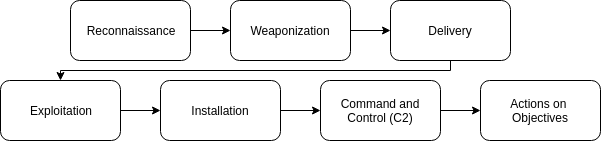
\includegraphics[width=.8\linewidth]{resource/img/ch_background/intrusion_kill_chain.png}
\caption{LM Intrusion Kill Chain\cite{Hutchins_Cloppert_Amin}}
\label{fig:background:kill_chain}
\end{figure} 

Attacks against networks can be motivated by many factors, but the effects generally fall into one of a handful of categories\cite{Chakrabarti_Govindarasu_2002}. Our threat model assumes an attacker originating outside the core network boundary intends to target a device within the core network, permitting the attacker to view or alter a victim's traffic. In other words, identifying the potential for \textit{eavesdropping} and \textit{tampering} is the focus of this research, and we address the limitations of modeling network \textit{disruption} later in this section. Table \ref{tab:threats} lists some common attack patterns against Layer 2 and 3 networks. In general these attacks are used to redirect a target's traffic through an asset controlled by the attacker, or to escalate the attacker's privileges on systems that interact with the target. We briefly review these attack classes here in order to present our Datalog models in the following sections.



% Vulns
\begin{table}[ht]
\centering
\captionsetup{justification=centering}
\caption{Potential Threats}
\resizebox{.4\textwidth}{!}{%
% \begin{small}
\begin{tabular}{@{}lll@{}}
\toprule
% Layer 2 & Layer 3  &  \\ \midrule
VLAN Hopping & ACL Bypass \\
STP Injection & BGP Hijacking \\
ARP Cache Poisoning & Route Table Poisoning &  \\
MAC Flooding & SYN Flooding &  \\
CAM Overflow & Packet Crafting &  \\
MAC/DHCP Spoofing & IP Spoofing &  \\
%MPLS Attachment Point &  IPSec AH/IKE \\ 
\bottomrule
\end{tabular}%
% \end{small}
}
\label{tab:threats}
\end{table}

We frame our threat discussion within Layers 2 and 3 of the OSI 7-layer model here for clarity, but don't limit our analysis to only these vectors. These attacks often aren't the goal of an attacker, but rather enable the attacker to reach their goal through the effects of the compromise. For example, traffic eavesdropping may reveal credentials for a privileged account on some other system the attacker has interest in. 



\begin{figure}[ht]
  \centering
% \noindent\begin{minipage}[t]{0.98\linewidth}
\begin{bytefield}[bitwidth=1em]{39}
% \begin{bytefield}{39}
\bitbox[]{35}{$\overbrace{\hspace{34em}}^{\text{\normalsize L1 Eth Packet (72--1530B)}}$} & \bitbox[]{4}{} \\
\bitbox[]{6}{} &
\bitbox[]{29}{$\overbrace{\hspace{28em}}^{\text{\normalsize L2 Eth Frame (64--1522B)}}$} \\
\bitbox[]{21}{} &
\bitbox[]{9}{$\overbrace{\hspace{10em}}^{\text{\normalsize L3 Packet (46--1500B)}}$}  & \bitbox[]{9}{}  \\
    \begin{rightwordgroup}{802.3 field}
       \bitbox{3}{Pre} &  \bitbox{3}{SFD}  & 
        \bitbox{4}{src}  & \bitbox{4}{dst} & 
        \bitbox{4}{VLAN}  & \bitbox{3}{len} &
        \bitbox{10}{Payload}  & \bitbox{4}{CRC}
         & \bitbox{4}{IPG} 
    \end{rightwordgroup} \\
    \begin{rightwordgroup}{Bytes in field}
    \bitbox[]{3}{7} &  \bitbox[]{3}{1}  & 
        \bitbox[]{4}{6}  & \bitbox[]{4}{6} & 
        \bitbox[]{4}{4}  & \bitbox[]{3}{2} &
        \bitbox[]{10}{46--1500}  & \bitbox[]{4}{4}
         & \bitbox[]{4}{12} 
     \end{rightwordgroup}
    % \\ \bitbox[]{8}{$\underbracebrace{\hspace{11em}}_{\text{\normalsize Header}}$}
\end{bytefield}
% \end{minipage}
 \caption{802.3 Ethernet Packet Layout}
  \label{fig:bits_802_3}
\end{figure}


\textbf{Layer 2 Attacks:} 
\begin{itemize}
\item CAM Overflow: Hardware switches use \textit{Content Addressable Memory} tables to map devices to the port they are connected to. When frames enter the ingress switch port, a CAM table entry is created for the source MAC address and port if it doesn't exist. The destination MAC address is found in the CAM table and the frame is forwarded out the associated port. If no destination entry is found the frame is flooded out all ports, and the CAM table is updated with the port the destination MAC responds from. The CAM is implemented in hardware and has a fixed size buffer. If an attacker can exhaust the CAM buffer by generating enough unique source addressed frames to fill the table, the switch will flood any traffic without an entry to every switch port, allowing an attacker to eavesdrop traffic from any connected device on the native VLAN. 
\item  ARP Spoofing: The \textit{Address Resolution Protocol}\cite{Plummer} maps Layer 2 MAC addresses to Layer 3 IP addresses. To find a MAC address for a given IP target, an ARP request is broadcast to all members of the local subnet. The owner of the IP address then sends an ARP reply containing their MAC address. RFC 826 allows for unsolicited ARP replies, meaning that any system on the local subnet can announce that they own any IP or MAC address without the address first being requested by a peer. An attacker announcing ownership of an address will receive all traffic destined for that address. 
\item VLAN Hopping: \textit{Virtual LANs} allow the creation of multiple logically separate broadcast networks over the same Layer 2 switch. The 802.1Q VLAN field in Figure \ref{fig:bits_802_3} accepts a 12 bit VLAN tag to differentiate 4094 possible VLANs, with later extensions to the standard allowing over 16 million tags. Since VLANs are isolated broadcast domains, communication between VLAN nodes must be routed over a Layer 3 protocol. VLAN tags are written to Ethernet frames by the ingress switch either statically based on attachment port, or dynamically based on some policy like the source MAC address. The primary VLAN connection types are \textit{Access} links which connect a host to a switch using a single tag, \textit{Trunk} links which interconnect switches and carry tags for all VLANs, and the default \textit{Native} VLAN which allows untagged traffic and is typically used for management. The link type is configured for each switch port manually over the management interface, dynamically using a protocol like DTP (dynamic trunking protocol), or it falls back to the default which is vendor and model specific. If a switch port the attacker is connected to is not explicitly configured as an Access port, the attacker can present themselves as a peer switching device (known as \textit{Switch Spoofing}) and craft the DTP packets to negotiate a Trunk port, resulting in access to traffic on any managed VLAN. Another VLAN bypass can be accomplished if the attacker is allowed to write arbitrary data to the VLAN tag field, which is permitted by members of the Native VLAN. In this scenario, an attacker can send traffic to a target on another VLAN by \textit{Double Tagging} messages. The outer VLAN tag is popped by the first receiving switch and then flooded out all of its Native VLAN ports. The inner tag is now read by the receiving switch and the message is sent to the victim. This is a blinded attack since no response will be returned from the malicious traffic.
% \item STP 
% \item DHCP
% \item MPLS
\end{itemize}

% \begin{figure*}
%   \centering
%   \begin{bytefield}{32}
%     \bitheader{31,24,23,16,15,8,7,0} \\
%     \bitbox{1}{\tiny{M\\E\\M}} & \bitbox{3}{SEL} & \bitbox{23}{} & \bitbox{4}{Mem\\Type} & \bitbox{4}{ID} \\    
%   \end{bytefield}
%   \caption{\label{fig:mwe_cmd}Cmd word}
% \end{figure*}


% \begin{figure}[ht]
%   \centering
% \begin{bytefield}[bitwidth=1em]{32}
%     \bitheader{0-31} \\
%     % \begin{rightwordgroup}{RTP \\  Header}
%         \bitbox{4}{V=6} & \bitbox{8}{Traffic Class} & \bitbox{20}{Flow Label} \\
%         \bitbox{16}{Payload Length}  & \bitbox{8}{Next Header} & \bitbox{8}{Hop Limit} \\
%     % \end{rightwordgroup} \\
%     \wordbox[tlr]{2}{128-bit Source Address} \\
%     \wordbox[tlr]{2}{128-bit Destination Address} \\
%     \wordbox[blr]{1}{$\cdots$} \\
% \end{bytefield}
%  \caption{IPv6 frame format rfc8200}
%   \label{fig:bits_ipv6}
% \end{figure}


% Layer 2 Attacks: 

% \input{content/background/infra/attacks/vlan_hopping.tex}

\label{sec:background:attack_modeling}


% \subsection{Graph Based Models}\label{sec:background:attack_graphs}

% 
Vulnerability exploitation can be thought of as a set of preconditions which must be true for an attack to be successful, and a set of postconditions that become true after a vulnerability is successfully exploited. In this context, an attack graph is a tool that can efficiently evaluate the set of preconditions that exist in a system and determine if attaining a specific postcondition is possible. When an attack goal is reachable in a system, the attack graph will enumerate all sequences of preconditions necessary to assert the goal’s postcondition is true. When the goal is not reachable, no attack graph is produced. To date, research in this area has focused on software vulnerabilities. A likely reason being that a large amount of data is collected and publicly disseminated in the form of the National Vulnerability Database. The NVD provides a number of metrics associated with each vulnerability along with metadata like access vector and potential effects. 

Modeling a system's vulnerabilities and the reachability between those vulnerabilities can be found in the literature as far back as 1994 with Dacier\cite{Dacier_1994} formalising the concept of privilege graphs and representing the translated graph as a Markov Model. Phillips and Swiler\cite{Phillips_Swiler_1998} present a separate attack graph generation method that can account for multi-stage attacks and attacker capabilities in 1998. In 1999 Ortalo\cite{Ortalo_1999}  provides experimental results and some fundamental metrics using Markov analysis with Dacier's privilege graphs, and in 2002 Sheyner\cite{Sheyner_Haines_Jha_Lippmann_Wing_2002} describes how attack graph construction and analysis can be automated. In 2006 Ou\cite{Ou_Boyer_McQueen_2006} provides an analysis of scalability extensions to the MulVal\cite{Ou_Govindavajhala_Appel} attack graph engine presented the previous year, and in 2013 Hong\cite{Hong_Kim_Takaoka_2013} presents further scalability improvements to MulVal using logic reduction techniques. In 2015 Abraham\cite{Abraham_Nair_2015b} introduces the Cyber Security Analytics Framework(CSAF) which we adopt for this analysis. More thorough surveys of the canonical attack graph literature can be found in \cite{Kordy_2013} and \cite{Lippmann_Ingols_2005}. %We use the remainder of this section to illustrate the MulVal inputs and outputs as expected by the CSAF. 

Attack graphs show the relationships among vulnerabilities within a system and provide context to security scans already conducted by many organisations. An attack graph is a directed graph that captures all possible paths an attacker can traverse within a system to reach a desired target state. The first node in the graph represents the origin of the attack and the final node denotes the target. The origin contains only outbound edges and the target contains only inbound edges. Nodes in the graph between the origin and target represent discrete states in states network. Each edge in the graph identifies a possible pivot from one state to another through either unaltered access mechanisms or successful exploitation of a vulnerability. The conditions necessary for successful compromise of the vulnerability are encapsulated in the attack graph vertices, and include information such as network, port, protocol, and access privilege level restrictions, as well as the effect of a successful exploit on the system such as privilege escalation or remote code execution. These conditions can be populated from the output of IA and network management systems, or in hypothetical cases, can be defined manually.  

%Our research extends the insight provided by an attack graph to draw conclusions about the security of a network through analyzing these vulnerability relationships and simulating an attacker’s progression through the network to a given target.   

% \begin{figure}[H]
% \centering
% \begin{adjustbox}{minipage=\linewidth,scale=0.6}
% \begin{subfigure}{.5\textwidth}
% \includegraphics[width=\linewidth]{img/eg_net.png}
% \caption{example network}
% \label{fig:eg_net}
% \end{subfigure}%
% \begin{subfigure}{.5\textwidth}
% %%\includegraphics[width=\linewidth]{img/1553187466080.png}
% 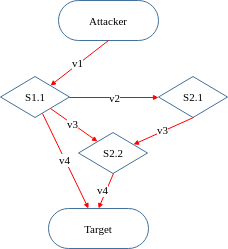
\includegraphics[width=\linewidth]{content/figs/eg_attack_graph_002a.png}
% \caption{resulting attack graph}
% \label{fig:eg_ag}
% \end{subfigure}%
% \caption{Attack Graph Example}
% \label{fig:eg}
% \end{adjustbox}
% \end{figure} 

% For example, Figure \ref{fig:eg_net} shows a fictional system being targeted by an attacker and Figure \ref{fig:eg_ag} shows the derived attack graph. While there exist 4 vulnerabilities between the attacker and the target, only vulnerability v1 is exploitable from the attacker’s original context. If this vulnerability is successfully exploited, the attacker can subsequently exploit vulnerabilities v2 or v3 on System 2 or proceed directly to the Target by exploiting v4. Note in Figure \ref{fig:eg_ag} that nodes S2.1 and S2.2 are separate vulnerabilities on the same system (System 2); nodes in an attack graph don’t necessarily have a one-to-one mapping to system elements. Also notice that there are three possible attack paths available for the attacker to reach the target.  


% The next step is to take the generated attack graph and augment transition probabilities based on an established or approximated CVSS score.  For example, we may choose exploitability, the measure of how easily a vulnerability is leveraged by an attacker, or impact, the measure of how critical an exploit would be to operations, to base the likelihood of an attack path being taken. Due to the large and complex graphs that can be generated for even simple networks, we automate the process of translating the attack graph output into a form that can be consumed by subsequent phases through a data transform pipeline to include graph node reduction, CVSS score lookup and assignment, and transition probability calculations.

The example in Figure \ref{fig:eg_net01} assumes an attacker located on the public internet with the target being root access on the internal workstation. The network model provided to MulVal is shown in Listing \ref{lst:input}. The $hacl/4$ clauses define access control rules that depict router and firewall configurations and dictate reachability between states. The host configuration properties include what services are running, the user or privilege level that service is running as, and any vulnerabilities known to affect that service.

\begin{figure}[ht]
\begin{tabular}{p{0.43\textwidth}p{0.51\textwidth}}
\begin{minipage}{.43\textwidth}
\centering
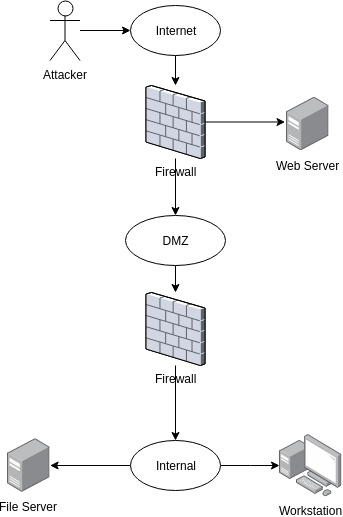
\includegraphics[scale=.47]{resource/img/ch_background/sdn_analytics/egarch_01.png}
\caption{Example network}
\label{fig:eg_net01}
%\end{figure} 
\end{minipage}
&
\begin{minipage}{.51\textwidth}
% \begin{adjustbox}{width=\textwidth}
\begin{lstlisting}[style=datalog, label={lst:input}, caption={input.P \cite{Ou_Boyer_McQueen_2006}}]
attackerLocated(internet).
attackGoal(execCode(workStation,_)).
hacl(internet, webServer, tcp, 80).
hacl(webServer, _,  _, _).
hacl(fileServer, _, _, _).
hacl(workStation, _, _, _).
hacl(H,H,_,_).
/* configuration information of fileServer */
networkServiceInfo(fileServer, mountd, rpc, 100005, root).
nfsExportInfo(fileServer, '/export', _anyAccess, workStation).
nfsExportInfo(fileServer, '/export', _anyAccess, webServer).
vulExists(fileServer, vulID, mountd).
vulProperty(vulID, remoteExploit, privEscalation).
localFileProtection(fileServer, root, _, _).
/* configuration information of webServer */
vulExists(webServer, 'CAN-2002-0392', httpd).
vulProperty('CAN-2002-0392', remoteExploit, privEscalation).
networkServiceInfo(webServer , httpd, tcp , 80 , apache).
/* configuration information of workStation */
nfsMounted(workStation, '/usr/local/share', 
   fileServer, '/export', read).
\end{lstlisting}
% \end{adjustbox}
\end{minipage}
\end{tabular}
\end{figure}

 The visual representation of the resulting attack graph can be found in Figure \ref{fig:tg_001}. A MulVal attack graph contains three types of nodes: \textbf{AND}, \textbf{OR}, and \textbf{LEAF}. \textit{LEAF} nodes (rectangles) describe known facts like configuration information and attacker privilege that are given as inputs to the system model. Internal nodes generally represent potential privileges to be gained by an attacker.  \textit{AND} nodes (ovals) contain interaction rules that dictate which facts and conditions are necessary to derive new knowledge. \textit{OR} nodes (diamonds) represent derived facts such as transition states possible given all incoming conditions are satisfied.

% \begin{figure}[ht]
% \centering
% \includegraphics[width=\linewidth]{content/figs/AttackGraph.eps}
% \caption{Resulting attack graph}
% \label{fig:eg_ag01}
% \end{figure} 

 A brief reading of the attack graph generated in Table \ref{tab:mulval_out} and Figure \ref{fig:tg_001} from the top left:
\setlist{nosep}
\begin{itemize}
\item An attacker from the internet (node 18) can access $webServer$ on port 80 (node 15)
\item Vulnerability CAN-2002-0392 can be exploited (node 20) to allow remote code execution on $webServer$ as user $apache$. From here the attacker can either (node 13):
\begin{enumerate}
\item Access $fileServer$ directly over rpc (node 10) and use this to escalate privilege to root (node 22) and write malicious files served to $workstation$ (node 5). 
\item $OR$ the attacker can write malicious files served to $workstation$ directly using NFS shell (node 23) 
\end{enumerate}
\item Given $workstation$ can access the malicious file (node 26) and the malicious file has been created (node 5) then $workstation$ can execute the malicious file with $root$ privileges allowing the attacker to achieve the target. 
\end{itemize}

\begin{table}[ht]
    \caption{MulVal gernerated output}
\begin{subfigure}[t]{0.6\textwidth}
\resizebox{\textwidth}{!}{%
\begin{tabular}[t]{@{}llll@{}}
\toprule
ID & Text & Type & Leaf \\ \midrule
1 & execCode(workStation,root) & OR & 0 \\ 
2 & RULE 4 (Trojan horse installation) & AND & 0 \\
3 & accessFile(workStation,write,'/usr/local/share') & OR & 0 \\
4 & RULE 16 (NFS semantics) & AND & 0 \\
5 & accessFile(fileServer,write,'/export') & OR & 0 \\
6 & RULE 10 (execCode implies file access) & AND & 0 \\
7 & canAccessFile(fileServer,root,write,'/export') & LEAF & 1 \\
8 & execCode(fileServer,root) & OR & 0 \\
9 & RULE 2 (remote exploit of a server program) & AND & 0 \\
10 & netAccess(fileServer,rpc,100005) & OR & 0 \\
11 & RULE 5 (multi-hop access) & AND & 0 \\
12 & hacl(webServer,fileServer,rpc,100005) & LEAF & 1 \\
13 & execCode(webServer,apache) & OR & 0 \\
14 & RULE 2 (remote exploit of a server program) & AND & 0 \\
15 & netAccess(webServer,tcp,80) & OR & 0 \\
16 & RULE 6 (direct network access) & AND & 0 \\
17 & hacl(internet,webServer,tcp,80) & LEAF & 1 \\
18 & attackerLocated(internet) & LEAF & 1 \\
19 & networkServiceInfo(webServer,httpd,tcp,80,apache) & LEAF & 1 \\
20 & vulExists(webServer,'CAN-2002-0392',httpd,remoteExploit,privEscalation) & LEAF & 1 \\
21 & networkServiceInfo(fileServer,mountd,rpc,100005,root) & LEAF & 1 \\
22 & vulExists(fileServer,vulID,mountd,remoteExploit,privEscalation) & LEAF & 1 \\
23 & RULE 17 (NFS shell) & AND & 0 \\
24 & hacl(webServer,fileServer,nfsProtocol,nfsPort) & LEAF & 1 \\
25 & nfsExportInfo(fileServer,'/export',write,webServer) & LEAF & 1 \\
26 & nfsMounted(workStation,'/usr/local/share',fileServer,'/export',read) & LEAF & 1 \\ \bottomrule
\end{tabular}%
}
\caption{VERTICES.csv}
\label{tab:eg_verts}
\end{subfigure}
\begin{subfigure}[t]{0.3\textwidth}
\flushright
\resizebox{.68\textwidth}{!}{%
\begin{tabular}[t]{@{}lll@{}}
\toprule
src vertex & dst vertex & weight \\ \midrule 
6  & 7  & -1 \\
11 & 12 & -1 \\
16 & 17 & -1 \\
16 & 18 & -1 \\
15 & 16 & -1 \\
14 & 15 & -1 \\
14 & 19 & -1 \\
14 & 20 & -1 \\
13 & 14 & -1 \\
11 & 13 & -1 \\
10 & 11 & -1 \\
9  & 10 & -1 \\
9  & 21 & -1 \\
9  & 22 & -1 \\
8  & 9  & -1 \\
6  & 8  & -1 \\
5  & 6  & -1 \\
23 & 24 & -1 \\
23 & 25 & -1 \\
23 & 13 & -1 \\
5  & 23 & -1 \\
4  & 5  & -1 \\
4  & 26 & -1 \\
3  & 4  & -1 \\
2  & 3  & -1 \\
1  & 2  & -1 \\ \bottomrule
\end{tabular}
}
\caption{ARCS.CSV}
\label{tab:eg_arcs}
\end{subfigure}
    \label{tab:mulval_out}
\end{table}

Along with the visualization in Figure \ref{fig:tg_001}, MulVal also produces comma separated value formatted output which lends itself more readily to further analysis. The lists of edges and vertices in Table \ref{tab:mulval_out} describe the attack graph generated from Listing \ref{lst:input}.

\section{Security Metrics}\label{sec:background:metrics}




\input{content/chapters/ch_background/sec_metrics/metrics_intro.tex}

\subsection{Existing Security Metrics Taxonomies}\label{sec:background:existing_metrics_taxonomies}

\input{content/chapters/ch_background/sec_metrics/existing_taxonomies}

\subsection{Security Metrics Taxonomy}\label{sec:background:metrics_by_cybok}

\input{content/chapters/ch_background/sec_metrics/sec_metrics_taxonomy.tex}

% \subsection{Graph Based Metrics}\label{sec:background:graph_based_metrics}

% \input{content/chapters/ch_background/sec_metrics/sec_metrics.tex}

% % \subsection{Metric Validation}\label{sec:background:metric_validation}

% % \input{content/chapters/ch_background/metric_validation.tex}

% % \section{Related Work}\label{sec:background:related}

% % \subsection{Structural Metrics} \label{subsec:struct_metrics}
% \input{content/chapters/ch_background/sec_metrics/structural_metrics.tex}

% % \subsection{Probabilistic Metrics} \label{subsec:prob_metrics}
% \input{content/chapters/ch_background/sec_metrics/prob_metrics.tex}

% 
NIST 800-55\cite{Swanson_Bartol_Sabato_Hash_Graffo_2003} describes security metrics as "\textit{tools designed to facilitate decision making and improve performance and accountability through collection, analysis, and reporting of relevant performance-related data. IT security metrics must be based on IT security performance goals and objectives.}" This section reviews some of the available security metrics from the literature loosely grouped by each Cybok heading, along with properties that have been used to characterize these metrics. 

% \subsection{Security Metrics Taxonomy}\label{sec:background:metrics_by_cybok}

% 
Above we reviewed some existing classification methods for security metrics. These included taxonomies from both narrow and broadly focused surveys. While there is certainly overlap within some of the categories and properties identified, there is also collision between similar sounding concepts from different sources. To remove ambiguity, and more importantly to address the immediate question, we can map all our security metrics onto the taxonomy derived from the Cyber Security Body of Knowledge. The CyBoK is an effort to collect and maintain canonical research across the entirety of the cyber security domain. Included in this mandate is keeping all of it organized, so we can presume that if there is a topic in security we would like to measure, then there will be a corresponding topic in the CyBoK to consult. 

Security metrics can be categorized by the area of cyber security to which they apply. In this respect, the security metric surveys available in recent literature are by nature focused narrowly on a specific subfield, such as cryptographic or software development lifecycle security metrics. To remove ambiguity in terms among surveys, we attempt to include these in a \textit{big-picture} view of the field of cyber security by classifying them under the general headings of the recently released Cyber Security Body of Knowledge\cite{Rashid_Chivers_Danezis_Lupu_Martin} depicted in Figure \ref{fig:intro:cybok}. By grouping our security metrics by Cybok category, we can determine our cyber security metric coverage, and use this context to identify non-security related metrics that would be relevant to the area. 

\subsubsection{Human, Organization, \& Regulatory Metrics}

\begin{figure}[ht]

\begin{mdframed}
\centering
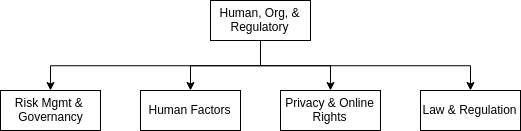
\includegraphics[width=.8\linewidth]{resource/img/ch_background/cybok_metrics/cybok_hor.png}
\end{mdframed}
\caption{Cybok: Human, Organization, \& Regulation Metrics
\label{fig:background:cybok_hor_metrics}}
\end{figure} 

\begin{figure}[ht]
\centering
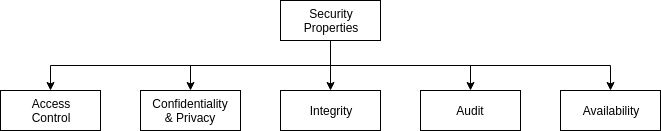
\includegraphics[width=.9\linewidth]{resource/img/ch_background/cybok_metrics/morrison_sec_props.png}
\caption{Most of Morrison’s class for Security Properties would fit under HO\&R.
\label{fig:background:cybok_hor_metrics_morrison}}
\end{figure} 

\begin{figure}[ht]
\centering
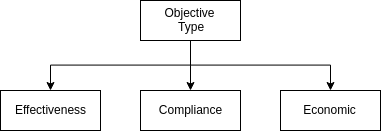
\includegraphics[width=.6\linewidth]{resource/img/ch_background/cybok_metrics/ramos_objective_type.png}
\caption{Ramos’ Objective Type metrics fall under HO\&R (economics is cross cutting).
\label{fig:background:cybok_hor_metrics_ramos}}
\end{figure} 


\begin{figure}[ht]
\centering
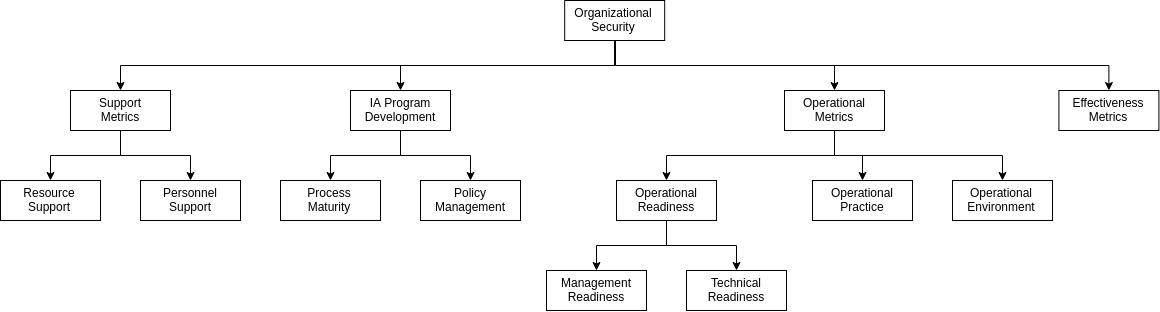
\includegraphics[width=.95\linewidth]{resource/img/ch_background/cybok_metrics/vaughn_org_metrics.png}
\caption{Vaughn’s Organization Security metrics subtree  falls under HO\&R.
\label{fig:background:cybok_hor_metrics_vaughn}}
\end{figure} 

Metrics in HO\&R are usually derived from applicable regulations and policies (ISO, FISMA, HIPPA, PCI, ADA, etc). Often these are counts or ratios that quantify the proportion of assets that are in/out of compliance with the regulation. Typical applications for these metrics are system audits (how many current users have completed mandatory training) or accreditations (how many of these secure operations checkboxes does the current system check).


\subsubsection{Attack \& Defense Metrics}

\begin{figure}[ht]

\begin{mdframed}
\centering
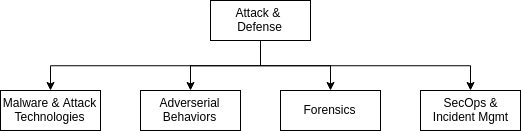
\includegraphics[width=.8\linewidth]{resource/img/ch_background/cybok_metrics/cybok_ad.png}
\end{mdframed}
\caption{Cybok: Attack \& Defense Domain Metrics
\label{fig:background:cybok_ad_metrics}}
\end{figure} 

Attack and defense describes many of the security metrics we have investigated in this thesis. Malware and Attack metrics can quantify an attacker’s capabilities, the DoS’ing bandwidth of a botnet or the number of accounts controlled are examples. Adversarial behaviours might relate to MITRE’s APT and CAPEC attack pattern datasets, but I haven’t encountered metrics that evaluate this yet (although it shows up regularly in threat models). Forensics metrics typically include time to unpack or deobfuscate a malware sample, or the amount of time to determine an indicator of compromise for IDS deployment. SecOps \& Incident Response metrics include standards from the literature such as IDS efficacy and mean time between failures. 

\begin{figure}[ht]
\centering
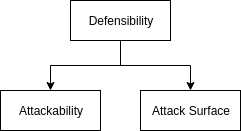
\includegraphics[width=.35\linewidth]{resource/img/ch_background/cybok_metrics/morrison_defensibility.png}
\caption{Morrison’s Defensibility metrics fall generally under A\&D.
\label{fig:background:cybok_ad_morrison}}
\end{figure} 

\begin{figure}[ht]
\centering
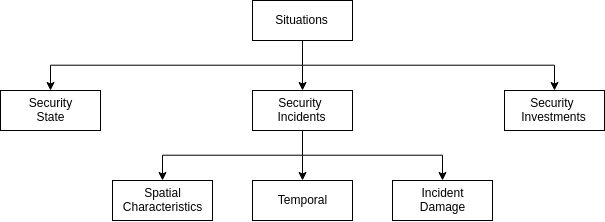
\includegraphics[width=.8\linewidth]{resource/img/ch_background/cybok_metrics/pendleton_situations.png}
\caption{Pendleton’s Situations metrics fall under A\&D.
\label{fig:background:cybok_ad_pendleton}}
\end{figure} 

\begin{figure}[ht]
\centering
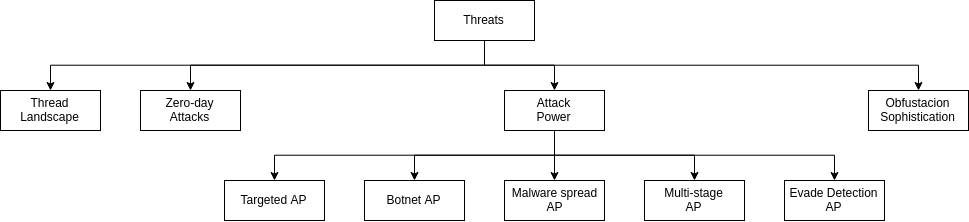
\includegraphics[width=.95\linewidth]{resource/img/ch_background/cybok_metrics/pendleton_threats.png}
\caption{Pendleton’s Threats metrics fall under A\&D.
\label{fig:background:cybok_ad_pendleton_threats}}
\end{figure} 

\begin{figure}[ht]
\centering
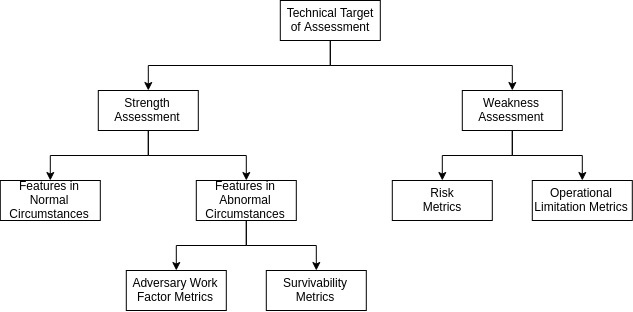
\includegraphics[width=.75\linewidth]{resource/img/ch_background/cybok_metrics/vaughn_ttoa.png}
\caption{Vaughn’s Strength and Weakness metrics fall under A\&D.
\label{fig:background:cybok_ad_vaugh_ttoa}}
\end{figure} 

\subsubsection{Systems Security Metrics}

\begin{figure}[ht]

\begin{mdframed}
\centering
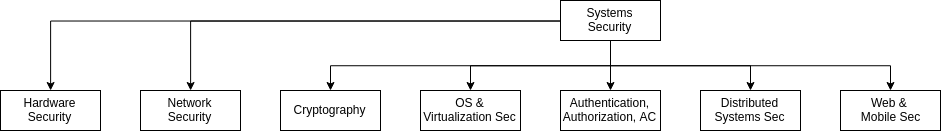
\includegraphics[width=.95\linewidth]{resource/img/ch_background/cybok_metrics/cybok_systems.png}
\end{mdframed}
\caption{Cybok: Systems Domain Metrics
\label{fig:background:cybok_sys_metrics}}
\end{figure} 

Systems security metrics span most aspects of operational security. Hardware and Network security metrics were discussed under infrastructure. Typical applications of cryptographic security metrics include all the formal verification artifacts involved in the validation of a protocol or implementation, along with performance, key size, entropy, etc. OS security metrics may be derived from common criteria/ EAL or measure isolation, weakness to side channels, or number of vulnerabilities known along with severity. 

\begin{figure}[ht]
\centering
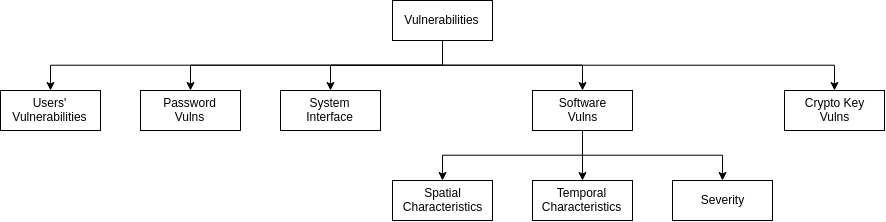
\includegraphics[width=.95\linewidth]{resource/img/ch_background/cybok_metrics/pendleton_vulns.png}
\caption{Pendleton’s Vulnerabilities security metrics fall under System’s security metrics
\label{fig:background:pendleton_vuln_metrics}}
\end{figure} 

Model based network security metrics classified by Ramos\cite{Ramos_Lazar_Filho_Rodrigues_2017} are shown in Figure \ref{fig:background:ramos_taxonomy}. These metrics are designated as Compliance based when a larger value indicates more security. Moment identifies if a measurement can be taken pre-deployment and remains static throughout operation, or if the metric is dynamic and should be measured repeatedly. Consistency distinguishes if the measured value relies on subjective human input or if its evaluation is objective. To compare with network performance metrics like latency or throughput, these security metrics are heavily influenced by subjective criteria. For example, the reliability based models make assumptions about an attacker’s success rate, level of effort, motivations, and capabilities that could change depending on who is filling in the weights. 

% \begin{minipage}{\linewidth}
% % \begin{table}[]
% \resizebox{\textwidth}{!}{%
% \begin{tabular}{@{}lllll@{}}
% \toprule
% \textbf{Metric} & \textbf{Compliance} & \textbf{Moment} & \textbf{Consistency} &  \\ \midrule
% MTTF {[}70{]}, {[}71{]} & compliance & dynamic & objective &  \\
% METF {[}72{]} & compliance & dynamic & subjective &  \\
% MTSF {[}40{]}, {[}73{]}, {[}74{]} & compliance & static & subjective &  \\
% MTFF {[}53{]}, {[}54{]} & compliance & static & subjective &  \\
% MTTC by McQueen et al. {[}8{]}, {[}75{]} & compliance & static & subjective &  \\
% MTTC by Leversage et al. {[}76{]} & compliance & static & subjective &  \\
% Steady-State Security {[}40{]}, {[}73{]}, {[}74{]} & non-compliance & static & subjective &  \\
% Reliability {[}79{]} & compliance & static & objective &  \\
% Success Likelihood {[}80{]} & non-compliance & dynamic & subjective &  \\
% q {[}81{]} & non-compliance & static & objective &  \\
% Shortest Path {[}83{]}, {[}10{]} & compliance & dynamic & objective &  \\ 
% Number of Paths {[}72{]}, {[}10{]} & non-compliance & dynamic & objective &  \\
% Mean of Path Lengths {[}95{]}, {[}10{]} & compliance & dynamic & objective &  \\
% Normalized Mean of Path Lengths {[}10{]} & compliance & dynamic & objective &  \\
% Assistive metrics: SDPL, MoPL, MePL {[}10{]} & compliance & dynamic & objective &  \\
% Weakest Adversary {[}96{]}  & compliance & static & subjective&  \\
% Network Compromise Percentage {[}97{]} & non-compliance &  dynamic &  objective &\\
% State Rank {[}98{]} & non-compliance & static & subjective &  \\
% Cumulative Score {[}99{]} & non-compliance & static & objective &  \\
% AGP {[}88{]} & non-compliance & static & subjective &  \\
% Attack Resistance {[}100{]} & compliance & static & subjective &  \\
% Enhanced Cumulative Score {[}102{]} & non-compliance & static & subjective &  \\
% Liu and Man’s metric {[}104{]} & non-compliance & dynamic & subjective &  \\
% Frigault and Wang’s metric {[}105{]} & non-compliance & static & subjective &  \\
% Frigault and colleagues’ metric {[}106{]} & non-compliance & dynamic & subjective &  \\
% Poolsappasit and colleagues’ metric {[}107{]} & non-compliance & dynamic & subjective &  \\
% Xie and colleagues’ metric {[}108{]} & non-compliance & dynamic & subjective &  \\
% Dantu and colleagues’ metric {[}109{]}, {[}110{]}, {[}111{]} & non-compliance & dynamic & subjective &  \\
% Expected Difficulty {[}112{]} & compliance & static & subjective &  \\
% VEA-bility {[}31{]} & compliance & static & subjective &  \\
% k-zero day safety {[}113{]}, {[}114{]} & compliance & static & subjective &  \\
% d2-Diversity (least attacking effort) {[}115{]}, {[}116{]} & compliance & static & subjective &  \\
% d3-Diversity (avg. attacking effort) {[}115{]}, {[}116{]} & non-compliance & static & subjective &  \\
% d1-Diversity (\% of distinct resources) {[}115{]}, {[}116{]} & compliance & static & subjective &  \\
% Seclius {[}118{]} & non-compliance & dynamic & objective &  \\
% Damage risk {[}120{]} & non-compliance & static & subjective &  \\
% Mean Privacy {[}121{]} & non-compliance & static & subjective &  \\
% Security Meter {[}122{]}, {[}123{]} & non-compliance & static & subjective &  \\
% Policy Security Score {[}124{]} & compliance & dynamic & subjective &  \\
% Probabilistic Vulnerability Measure {[}125{]} & non-compliance & dynamic & subjective &  \\
% Attack Propagation {[}126{]} & non-compliance & dynamic & subjective &  \\
% ADVISE {[}127{]} & compliance & static & subjective &  \\ \bottomrule
% \end{tabular}%
% }

% % \caption{Ramos}
% % \label{tab:ramos_metrics}
% % \end{table}
% \end{minipage}


\subsubsection{Infrastructure Security Metrics}

\begin{figure}[ht]

\begin{mdframed}
\centering
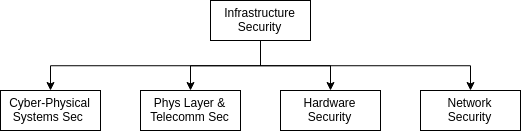
\includegraphics[width=.75\linewidth]{resource/img/ch_background/cybok_metrics/cybok_infra.png}
\end{mdframed}
\caption{Cybok: Infrastructure Domain Metrics
\label{fig:background:cybok_infra_metrics}}
\end{figure} 


Infrastructure Metrics to evaluate hardware security can be found in Rostami’s survey\cite{Rostami_2013, Rostami_Koushanfar_Karri_2014}. The majority of these are incident counts or ratios of expected to actual values, although analytical calculations (Hamming distances) are suggested to measure the amount of divergence from a known good source in several proposed metrics. Assuming the gold standard is available against which these measurements can be taken, they will evaluate the measurement empirically and deterministically. These metrics are similar to their performance related counterparts (eg, SPEC CPU) in that the performance increase over or under a reference system can be represented as a ratio of the two values. 

Cyber-Physical Systems (CPS) includes SCADA and other control systems, vehicle networks, and IoT systems that fall outside the scope of this thesis but certainly have applicable security metrics associated with attack surface and information leakage. Similarly, most aspects of the other infrastructure components listed above are captured in the system and threat model and included in the Attack \& Defense security metrics. Types of security metrics applicable here but not listed in the surveys above might include supply chain vulnerabilities, weakness to eavesdropping or side channel attacks. 



\subsubsection{Software \& Platform Security Metrics}

\begin{figure}[ht]

\begin{mdframed}
\centering
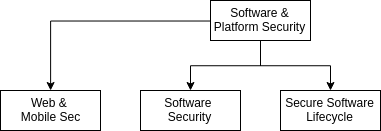
\includegraphics[width=.55\linewidth]{resource/img/ch_background/cybok_metrics/cybok_sw_platforms.png}
\end{mdframed}
\caption{Cybok: Software \& Platforms Domain Metrics
\label{fig:background:cybok_sw_metrics}}
\end{figure} 

Software security metrics were the focus of Morrison’s survey and apply here broadly. Typical applications of these type metrics derive from static analysis and test coverage. Of specific interest in the thesis is the remediation velocity, which measures the time between discovering a flaw in software and the time a fix has been merged into the code base.


\begin{figure}[ht]
\centering
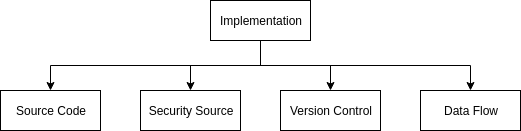
\includegraphics[width=.85\linewidth]{resource/img/ch_background/cybok_metrics/morrison_implementation.png}
\centering
\caption{Morrison’s Implementation Security metrics fall under SW\&P.
\label{fig:background:morrison_implementation_ad}}
\end{figure} 

% \subsubsection{Systems Security Metrics}

\subsection{Summary}

In the surveys summarized above there were over 500 distinct security metrics identified. The surveys each provided their own classification systems which were appropriate for the analysis they conducted, but none of these taxonomies generalize well to classify all types of security metrics. In this section we have described properties common to all metrics, identified overlaps in the various taxonomies, identified points of confusion between existing metric hierarchies, and described a suitable and intuitive system for classifying any current or future security metric. By using the Cybok as the underlying classification system we are also able to determine the distribution of metrics in each topic and identify areas of limited coverage which would benefit from future research.








% \subsection{Graph Based Metrics}\label{sec:background:graph_based_metrics}

% 



\begin{table}[ht]\centering
\caption{Metrics Summary\label{tab:metric_summary}}
% \addcontentsline{lot}{table}{Metrics Summary}
\resizebox{.8\textwidth}{!}{%
\begin{tabular}{@{}lp{.35\linewidth}l@{}}
\toprule
Metric Class & Description & Common Measurements \\ \midrule
Structural & Metrics based on the structure of the attack graph; used to identify attributes like shortest path, mean path length, or total number of paths. & SP, NP, MPL \\
Time-Based & Metrics that quantify time expectations for attributes like compromise, recovery, or incident response. & MTTF, MTTB, MTTR \\
Probability-Based & Metrics that associate probabilities attack paths to quantify the security of the network. & NR, PP, EPL \\
Temporal & Metrics that examine  vulnerability age on the system. & TAG \\ \bottomrule
\end{tabular}%
}
\end{table}

% \input{content/chapters/ch_background/sec_metrics/main.tex}

% \begin{table}[H]
% \begin{tabular}{p{3.2cm}p{8cm}p{3cm}p{3cm}}
% %{@{}llll@{}}
% \toprule
% Metric Class & Description & Common Measurements   \\ \midrule
% Structural & Metrics based on the structure of the attack graph; used to identify attributes like shortest path, mean path length, or total number of paths. & SP, NP, MPL   \\
% Time-Based  & Metrics that quantify time expectations for attributes like compromise, recovery, or incident response. & MTTF, MTTB, MTTR   \\
% Probability-Based  & Metrics that associate probabilities attack paths to quantify the security of the network. & NR, PP, EPL   \\
% Temporal & Metrics that examine  vulnerability age on the system. & TAG   \\ \bottomrule
% \end{tabular}
% \caption{Metrics Summary}
% \label{tab:metric_summary}
% \end{table}

\subsection{Analytics Pipelines}\label{sec:background:csaf}


\input{content/chapters/ch_background/metric_pipelines/pipeline_intro}

\subsubsection{CSAF}\label{sec:background:csaf}

\input{content/chapters/ch_background/metric_pipelines/csaf}

\subsubsection{Graph Based Metrics}\label{sec:background:graph_based_metrics}

\input{content/chapters/ch_background/sec_metrics/sec_metrics.tex}

% \subsection{Metric Validation}\label{sec:background:metric_validation}

% \input{content/chapters/ch_background/metric_validation.tex}

% \section{Related Work}\label{sec:background:related}

% \subsection{Structural Metrics} \label{subsec:struct_metrics}
\input{content/chapters/ch_background/sec_metrics/structural_metrics.tex}

% \subsection{Probabilistic Metrics} \label{subsec:prob_metrics}
\input{content/chapters/ch_background/sec_metrics/prob_metrics.tex}


% \subsection{Metric Validation}\label{sec:background:metric_validation}

% 
In \cite{Verendel_2009} Verendel finds 4 distinct validation methods used across the 90 security metrics papers surveyed: hypothetical, empirical, simulation, and theoretical. The author adds the caveat that no attempt was made to verify the quality of results, only to describe the methods used in each paper to substantiate the findings. In this thesis we demonstrate a framework for validating security metrics through empirical means. Specifically, 
\cite{Sonmez_2019}

% \section{Related Work}\label{sec:background:related} %\label{ch:background}
% \chapter{Related Work}

\section{MITRE ATT\&CK Framework}\label{sec:related:mitre}

\section{MulVal Infrastructure Modeling}\label{sec:related:mulval}

\section{PKB}\label{sec:related:pkb}\label{ch:subil}
% \chapter{Related Work}

\section{MITRE ATT\&CK Framework}\label{sec:related:mitre}

\section{MulVal Infrastructure Modeling}\label{sec:related:mulval}

\section{PKB}\label{sec:related:pkb}\label{ch:post_subil}

% \part{Current}\label{part:current}

\chapter{Automation Driven Security Measurement} \label{ch:automation}

% Observation is the foundation of scientific experimentation, and it becomes a measurement when they are quantified with respect to an agreed upon scale, or measurement unit. 
A number of metrics have been proposed in the literature which attempt to quantify some property of cyber security, but no systematic validation has been conducted to characterize the behaviour of these metrics as measurement instruments, or to understand how the quantity being measured is related to the security of the system under test. In Chapter \ref{ch:background} we broadly classified the body of available security metrics against the recently released Cyber Security Body of Knowledge, and identified common attributes across metric classes which may be useful anchors for comparison. In this chapter we propose a general four stage evaluation pipeline to encapsulate the processing specifics of each metric, encouraging a separation of the actual measurement logic from the model it is often paired with in publication. Decoupling these stages allows us to systematically apply a range of input models to a set of metrics, and we demonstrate some important results in our proof of concept. First, we determine a metric's suitability for use as a measurement instrument against validation criteria like operational range, sensitivity, and precision by observing performance over controlled variations of a reference input. Then we show how evaluating multiple metrics against common reference sets allows direct comparison of results and identification of patterns in measurement performance. Consequently, development and operations teams can also use this strategy to evaluate security tradeoffs between competing input designs (which we show in the case study in Section \ref{sec:case_studies:att}) or to measure the effects of incremental changes during production deployments (which we show in Chapter \ref{ch:benchmarking}). 

% The motivation of this thesis is to make modern information systems more secure, and the driving force behind that goal is automation. Many of the problems addressed in this work stem from the disparate ecosystem of tools, APIs, methodologies, libraries, and frameworks that exist in relative isolation to one another. Consider Security Information and Event Management (SIEM) systems as an example, which provide correlation of host/network event logs, IDS/IPS alerts, threat/vulnerability feeds, etc, and present a unified view of the system’s security posture automatically to the SOC. Before the advent of managed SIEMs, sys admins typically filled the role of security engineers, and relied on hand rolled collections of shell/perl scripts to manage systems, parse logs, collect or push events, format reports, and issue alarms. To be effective required tribal knowledge along with proficiency in programming, network plumbing, and systems management, so changes to the environment or workforce made it extremely difficult(expensive) to deliver continuous monitoring capabilities to operators at any scale. 

% We are in a similar state today with network design and enterprise planning. Infrastructure-as-Code, SDN, virtualization and containerization are all critical components in modern deployments, but the glue that ties them together is largely ad-hoc, and risk evaluation is still a manual task. In order to understand the security posture of a system even before it is rolled out and SIEMs are in place, we have created a tool to facilitate the automated analysis, collection, correlation, and dissemination of the security metrics mentioned above. The necessity of such a tool is critical to evaluating the efficacy of the metrics reviewed above, and provides the foundation for ongoing research in machine learning models for secure systems planning, design, and evolution as demonstrated in Chapter \ref{ch:ml}.


% If we measure an aspect of security before and after a change takes place, then we can quantify the impact that change had on security. If we test an aspect of cyber security at regular intervals, then we can determine the average rate of change for that security metric over the given time period. In order to sample security measurements at regular (approaching continuous) intervals, we assert that the test apparatus must be fully automated. Using the 5 basic CyBOK categories as a guide, we can briefly identify some types and familiar sources of available security metrics and describe the suitability to automation for each.

% \begin{theorem}\label{theo:intro:secmet_diff}
% If we measure an aspect of security before and after a change takes place, then we can quantify the impact that change had on security.
% \end{theorem}

% \begin{theorem}\label{theo:intro:secmet_rate}
% If we test an aspect of cyber security at regular intervals, then we can determine the average rate of change for that security metric over the given time period.
% \end{theorem}

% Theorems \ref{theo:intro:secmet_diff} and \ref{theo:intro:secmet_rate} establish the basis for a \textit{cyber security calculus} that are a central premise of this work. 


\section{Security Metrics Implementation}\label{sec:automation:secmet_impl}


Our architecture for implementing security metrics is straight forward. We declare a \textit{base security metric} type from which all metrics inherit three methods: 
\begin{itemize}
\item CheckPreReqs: is invoked either directly by the caller or in the calculate method to ensure all items necessary for the calculation are present.
\item Calculate: returns the resulting measurement
\item GetMetadata: returns the environment and ancillary data used during the calculation 
\end{itemize}
 
\begin{figure}[H]
\centering
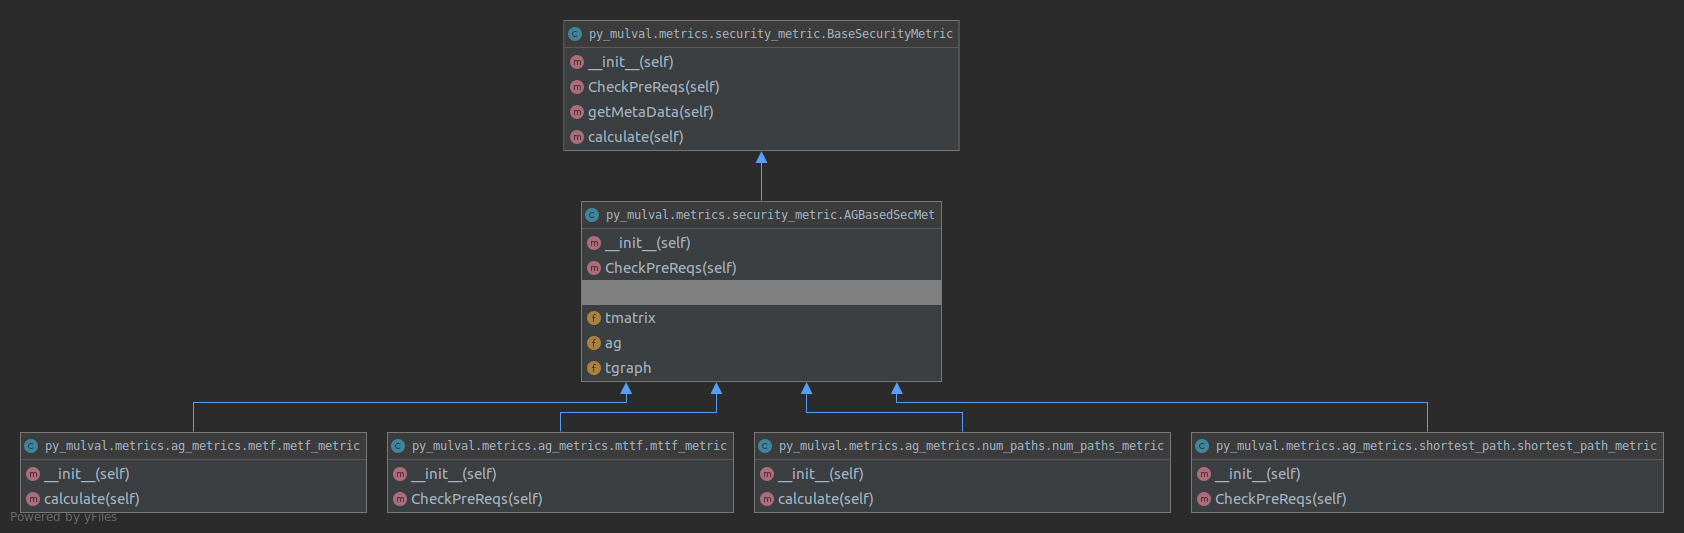
\includegraphics[width=.95\linewidth]{resource/img/ch_automation/metrics_class_uml.png}
\caption{Metric Class Diagram}
\label{fig:automation:metric_uml}
\end{figure} 

Figure \ref{fig:automation:metric_uml} shows the inheritance hierarchy for attack graph based security metrics. Each AG metric implementation inherits from AGBasedSecMetric which in turn inherits from BaseSecurityMetric. AGBasedSecMetric includes a property for attack graph which is a requirement to perform the metric calculation. Each BaseSecurityMetric also contains immutable properties for the name of the metric, the expected measurement unit for results, a citation field linking to the source paper where we found the metric, and a short summary of what the metric does. All these properties plus any additional information derived during calculation are added to the metadata dictionary of the metric and returned when the calculate method is called. 


\begin{figure}[H]
\centering
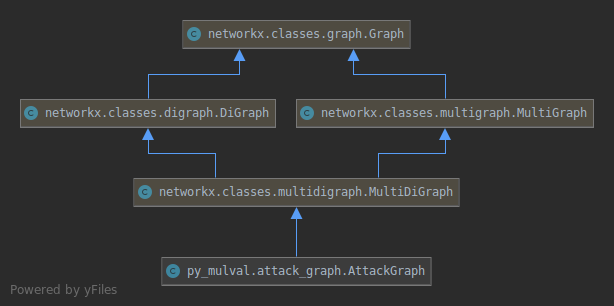
\includegraphics[width=.95\linewidth]{resource/img/ch_automation/attack_graph_simple_uml.png}
\caption{Attack Graph Class Diagram}
\label{fig:automation:ag_uml}
\end{figure} 

The attack graphs described in the literature vary somewhat in structure among implementations. For example, the AGs presented in \cite{Ou_Appel_2005} include non-exploits along with exploits as nodes with edges representing lateral movements. In \cite{Noel_Jajodia_2014} the non-exploit nodes don't appear to be present in the publication, although the TVA tool isn't publicly available to test this. In \cite{Dacier_1994} and \cite{Ortalo_1999} nodes represent system privileges and edges contain exploits that grant an attacker additional privileges on a set of systems, while in \cite{Phillips_Swiler_1998} edges carry probabilities of exploitation and the nodes represent actual hosts. While the differences are subtle, they are enough to necessitate a general form of attack graph which we present in Figure \ref{fig:automation:ag_uml}. Our representation of an attack graph is a multi-edged directed acyclic graph.     

% \begin{wrapfigure}[10]{I}{.25\textwidth}
\begin{figure}[H]
\centering
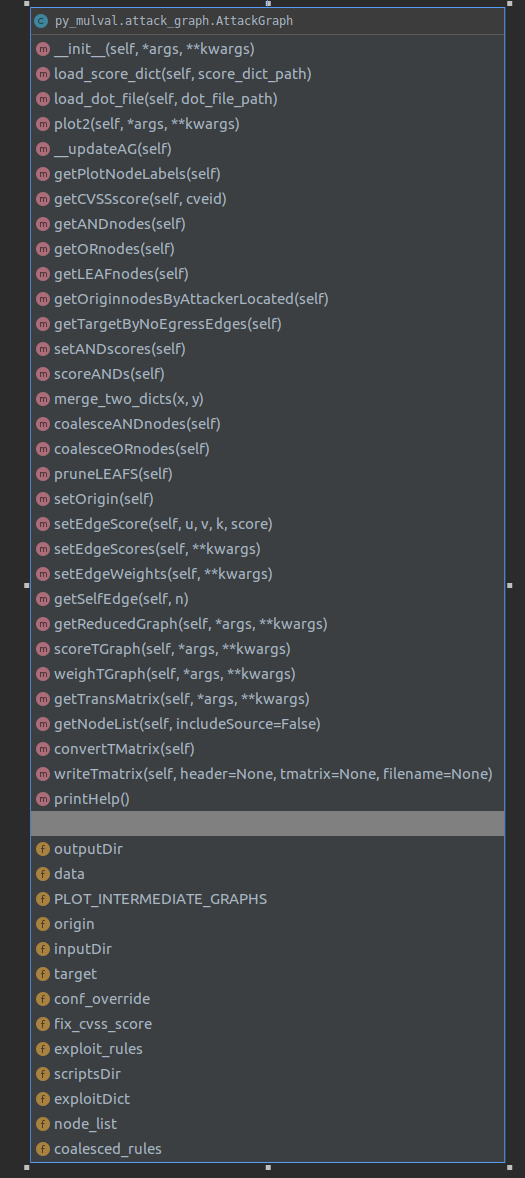
\includegraphics[scale=.45]{resource/img/ch_automation/attack_graph_class_diag.png}
% \end{wrapfigure}
\caption{Attack Graph Methods and Properties}
\label{fig:automation:ag_details_uml}
\end{figure}

As shown in Figure \ref{fig:automation:ag_details_uml}, our implementation allows us to load various AG formats from graph description language (.dot) files, from adjacency lists as shown in Tables \ref{tab:eg_verts} and \ref{tab:eg_arcs}, or other formats as specified. Once loaded, we provide programmatic access to manipulate scoring and weighting functions, exploits definitions, and vulnerability scores. This allows for a simple means to test the range of values a metric will generate, the sensitivity of a metric to fluctuations in parameters, and how well a metric performs on different models. It also gives us some insights into how well each AG type actually models threat and defense attributes.


In the \textit{Input} stage of Figure \ref{fig:automation:metric_pipeline}, system details depicted above the inbound arrows on the left are parsed into a model which describes the current environment or environment under test. Model parameters can be populated synthetically or from a live system. Rules comprising the threat model which describes how these components are allowed to interact with each other and with external stimulus can be added here for metrics that require it. The raw inputs to the processing pipeline can vary widely depending on which security metrics are being considered. At a high level, we treat the input stage as a black box for handling information requests from subsequent stages. This affords us the freedom to connect static data for testing and experimentation, and live data for production deployments without altering the contract or interface. In practice input targets can be existing APIs provided by SIEMs, query interfaces to a configuration database, source code repositories, vulnerability information feeds, generated network topologies, etc. At this stage we only assume appropriate adapters exist to make this data available for the subsequent stages.

The \textit{Pre Process} stage transforms the current knowledge base into a format suitable for the desired metric calculation. 

\begin{figure}[ht]
\centering
\includegraphics[width=.5\linewidth]{resource/img/ch_benchmarking/secmet_ptah/Ptah_archs.png}
\caption{Preprocessing and Transformation Handlers (\textbf{PTaH})}
\label{fig:automation:ptah_arch}
\end{figure} 

In metrics that compute aggregates, ratios, or simple statistics from findings and system facts, preprocessing steps may be minimal or bypassed entirely. In more complex metrics, such as those which consider the relationships between components or vulnerabilities, it may be necessary to craft the inputs expected from some composition of system facts along with some composition or chain of metric dependencies. In particular, metrics based on attack graphs and attack nets tend to make assumptions about the input structure which can be managed in this layer. We create these structures, score transitions, apply weights and mappings, and perform any other manipulations of our knowledge base in this layer to adhere to the input assumptions of particular metrics in this layer. 


The \textit{Compute} stage implements the calculation of the security metric and takes the measurement of the current state. 

The surveys covered in Section \ref{sec:litreview} describe properties common to all the security metrics they consider, which become evaluation criteria for their review. All security metrics inherit from a parent metric class that defines these common properties and the current system model, along with housekeeping functions and metadata like citations and usage.The security metric does not contain logic to create the inputs it operates on, so we can stack metrics to run in parallel against a single source of facts, or chain them in a processing pipeline to compose more complex analytics. 



Finally, the \textit{Reporting} stage handles the response logic needed to return the measured value and associated metadata appropriately. In our experience, most security metrics return a single value, although heuristics are also supported as bucket sizes and value count arrays returned within the accompanying metadata. 

% In order to experiment with different network architectures and exploit effects, it was necessary to reproduce each step in the process: 
% Install AG suite (MulVal, XSB) $\rightarrow$ Define AG input model (Datalog/Prolog) $\rightarrow$ Generate AG (Java, C++, ANTLR4, sed) $\rightarrow$ Import NVD (JSON, XML $\rightarrow$ SQL) $\rightarrow$ Implement custom adaptor for Stochastic Model expected input (Python, inference) $\rightarrow$ Insert transition matrix into provided R script (ctrl+c, ctrl+v) 
% After following this process precisely 2 times we understood why the AG based analytics community isn’t larger. Our immediate solution was to create a set of ansible roles and plays to automate the environment setup, test execution, and results collection entirely with a single command. This in itself lowers the barrier to entry for anyone interested in experimenting with attack graphs or looking to (quickly) reproduce our results.

% \begin{figure}[ht]
% \includegraphics[width=.48\textwidth]{img/Ptah_archs.png}
% \caption{Preprocessing and Transformation Handlers (\textbf{PTaH})}
% \label{fig:automation:ptah_arch}
% \end{figure} 


% To handle the scale and volume of requests needed to support the advanced use-cases listed below, we are currently implementing and evaluating the following features in the SMaaS architecture:
% Metric Isolation: Each metric should be independently deployable to allow scaling up and down as request volume dictates. Currently metrics are bundled in Python and R modules with logical separation at the function level.






\section{Interaction Rules for Infrastructure}\label{sec:automation:infra}


% \input{content/contrib/inrfa/main.tex}

% \input{content/contrib/inrfa/infra_attacks.tex}

% \input{content/contrib/inrfa/infra_model.tex}




The system model used by MulVal abstracts network infrastructure into a set of access control rules of the form \verb|hacl(_src, _dst, _prot, _port)|. This \verb|hacl/4| is a MulVal atomic \textit{primitive}, which to us means that it should be provided as input to the run. Horn clauses\cite{Chandra_Harel_1985} of the form $A\xleftarrow[]{} B_1, B_2,\dots, B_n $ are the foundation of MulVal's reasoning system. \textit{Facts} (primitive or derived) on the right-hand-side specify a relationship described by the term on the left-hand-side. \textit{Interaction Rules} in the framework wrap the Horn clause in a tuple with description and labeled weight metadata needed for attack graph processing and rendering. We use the terms interchangeably within this paper unless otherwise noted, and present the unwrapped form when discussing interaction rules for clarity.  The following Horn clause derives facts about network accessibility:
 \begin{verbatim}
 netAccess(P, H1, H2, Protocol, Port) :- execCode(P, H1 _User),
                                         hacl(H1, H2, Protocol, Port).
 \end{verbatim}
This statement can be read: \textit{Principal \textbf{P} has network access from host \textbf{H1} to host \textbf{H2} on \textbf{Port} using \textbf{Protocol} if \textbf{P} can execute code on \textbf{H1} as \textbf{\_User} and \textbf{H1} has access to \textbf{H2} over that \textbf{Port} and \textbf{Protocol}}. An interaction rule provides results for a single query on a relationship. A logic program is a collection of Horn clauses sufficient to cover a desired query space. In MulVal, \verb|meta(attackGoal(_))| is defined up front as the program objective, with the query \verb|findall(Goal, attack_simulation(Goal), L)| responsible for collecting attack traces. 

\begin{lstlisting}[style=datalog, label={lst:mulval_primitives}, caption={Mulval Primitive and Derived Facts}]
primitive(inCompetent(_principal)).
primitive(competent(_principal)).
primitive(clientProgram(_host, _programname)).
primitive(vulExists(_host, _vulID, _program)).
primitive(vulProperty(_vulID, _range, _consequence)).
primitive(hacl(_src, _dst, _prot, _port)).
primitive(attackerLocated(_host)).
primitive(hasAccount(_principal, _host, _account)).
primitive(networkServiceInfo(_host, _program, _protocol, _port, _user)).
primitive(setuidProgramInfo(_host, _program, _owner)).
primitive(nfsExportInfo(_server, _path, _access, _client)).
primitive(nfsMounted(_client, _clientpath, _server, _serverpath, _access)).
primitive(localFileProtection(_host, _user, _access, _path)).
primitive(dependsOn(_h, _program, _library)).
primitive(installed(_h, _program)).
primitive(bugHyp(_,_,_,_)).
primitive(vulExists(_machine,_vulID,_program,_range,_consequence)).
primitive(canAccessFile(_host, _user, _access, _path)).
primitive(isWebServer(_host)).

derived(execCode(_host, _user)).
derived(netAccess(_machine,_protocol,_port)).
derived(canAccessHost(_host)).
derived(accessFile(_machine,_access,_filepath)).
derived(accessMaliciousInput(_host, _principal, _program)).
derived(principalCompromised(_victim)).
derived(dos(_host)).
derived(logInService(_host, _protocol, _port)).
\end{lstlisting}

There is no explicit definition for network infrastructure in MulVal, but there is also no syntax requirement to adhere to the variable naming semantics. Remember that Prolog variables begin with either an upper case letter, or an underscore ('\_'),  and that constants begin with lower case letters. Thus we are free to overload the existing \verb|hacl/4|, and \verb|netAccess/4| predicates to define the Layer 2 and 3 network elements for our desired system model.

\begin{verbatim}
  hacl(sw1_xe_1_0_2, sw2_xe_1_1_1, vlan, ac_10_20).   
  hacl(sw1_et_1_0_1, sw_et_1_0_2, vlan, tr_30). 
  hacl(st2_ge_1_0_2, sw1_ge_1_1_1, vlan, mgmt_1). 
  hacl(rt2_ge_1_1_2, _, bgp, 179). 
  hacl(rt2_ge_1_1_2, ospf_grp_1, ospf, 179).
  hacl(rt3_ge_1_1_2, ospf_grp_1, ospf, 179).
\end{verbatim}

% We are aware of efforts\cite{Bacic_Froh_Henderson_2006,Henderson_Bacic_Froh_2005} to define these network elements as extensions to MulVal; however, we find the existing Datalog structures sufficient for our analysis without modifying the underlying model. We briefly discuss our reasoning and refer to the core and edge network designs found in \cite{Donovan_Prabhu_2017} for reference. 

%MulVal is primarily concerned with application layer attacks, with the primary effects of a successful attack being remote code execution and privilege escalation. In core and transit networks, the target is typically DoS, hijacking, or eavesdropping.The types of attacks we intend to model influence our syntax decisions.

For example, we can describe switches and routers along with their associated protocols without modification of the existing MulVal rules. This makes intuitive sense since the distinction between these devices becomes less clear when their functionality is virtualized. Having a VM running OpenVSwitch talking to a Layer 3 physical switch over Spanning Tree Protocol shouldn't require separate definitions from Layer 2 switches participating in the same protocol. Note this doesn't imply the attack surfaces are the same, and in Secion \ref{ch:background} we make this distinction explicitly. In the examples above we show how existing \verb|hacl/4| primitives can be used to specify VLAN tagged switch ports and OSPF areas for routers ports. The general naming convention to describe elements is underscore delimited, with the first entry describing the element (rt: router, sw: switch, rr: route reflector, ce: customer edge, pe: provider edge, p: provider core). Remaining fields identify the line card, interface, and port uniquely in a device and can be inherited from the organizations standard nomenclature. 

MulVal assumes attacker privilege is monotonically increasing, meaning that through the course of an attack an intruder can not decrease system access through vulnerability exploitation. This is a known\cite[Ch 2.6]{Ou_Appel_2005} effect inherited from Datalog and largely precludes the study of denial-of-service type attacks using the CSAF. That said, the types of attacks we can model using existing constructs still cover a broad range of Layer 2 and Layer 3 vulnerability classes which we define specifically in Section \ref{ch:background}.  


Defining the router interfaces as unique \verb|host| entries with distinct \verb|hacl/4| parameters permits us to treat exploit consequences like we would any other system. As an example, consider a provider edge router with an improperly configured access control list. If an attacker located within the attached customer edge network can discover this configuration error, the model reflects the new \verb|netAccess/5| state. In some tests we declare control, data, and management plane interface groups for each device to represent interface groups for simplicity. This naively represents the functionality an attacker would potentially target. By modeling the infrastructure devices this way we can define services on any plane as \verb|networkService/5| and express a compromise leading to unauthorized access of a different plane clearly for use in our trace analysis. 



\section{Deployment Automation}\label{sec:automation:deploy}


We use ansible\cite{Hall:2013:ACM:2601666} roles and playbooks to assist in running experiments for multiple input models. The roles we created set up a clean environment with MulVal installed on all inventory hosts. Since MulVal is no longer actively maintained, automating the deployment with ansible provides a reproducible environment that allows us to fix dependencies at the required version, track patches necessary to accommodate ongoing updates to linked projects like XSB and the NVD, and maintain and deploy custom interaction rules under version control. The playbooks we developed allow us to customize the CSAF analysis pipeline by simply including modules for each step in the process. As shown in Listing \ref{lst:playbook}, task lists representing modules can be as granular as necessary. Execution dependencies are defined by tags, allowing us to specify run targets and requirements selectively. For example, we can avoid duplicating time consuming tasks like downloading and preparing the CVSS DB, set the environment to a known state for development and debugging, or prepare and deploy results for consumption by other tools such as SIEM systems or monitoring dashboards. 

% \begin{figure}[H]
% \centering
% 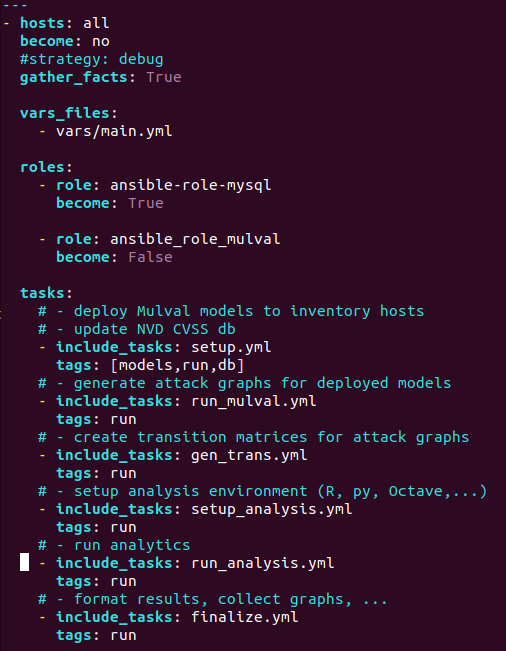
\includegraphics[width=.5\linewidth]{content/figs/deploy_infra/play.png}
% \caption{CSAF playbook}
% \label{fig:play}
% \end{figure} 

\begin{minipage}{\linewidth}
\begin{lstlisting}[language=yaml, label={lst:playbook}, caption={Ansible CSAF play},captionpos=b, linewidth=.9\textwidth]
- hosts: all
  become: no
  #strategy: debug
  gather_facts: True
  vars_files:
    - vars/main.yml
  roles:
    - role: ansible-role-mysql # NVD CVSS DB
      become: True
    - role: ansible-role-mulval # setup MulVal, XSB, etc
      become: False
  tasks:
    - include_tasks: setup.yml  # deploy models update NVD db
      tags: [models,run, db]
    - include_tasks: run.yml # generate attack graphs
      tags: [run, cleanup]
\end{lstlisting}
\end{minipage}

When preparing the target system, a directory containing the MulVal models to analyze is expected. These models are copied to the target system in individual directories as shown in Listing \ref{lst:model_dirs} since we can't control the output file names chosen by MulVal without modifying the distribution. 
% \begin{minipage}{1\linewidth}[ht]
\begin{lstlisting}[language=yaml, label={lst:model_dirs}, caption={MulVal distinct run dirs},captionpos=b, linewidth=.9\textwidth]
- name: copy models to remote in individual directories
  copy:
    src:  "{{item.path | relpath('{{mulval_models_src}}')}}"
    dest:  "{{mulval_models_dir}}/{{(item.path|basename|splitext)[0]}}"
  with_items: "{{find_results.files}}"
  tags: [models,run]
\end{lstlisting}
% \end{minipage}

MulVal supports a single custom interaction rules file being passed as a runtime argument. To allow for a more customizable custom rules set, we allow for the rules defined per model or globally as shown in Listing \ref{lst:custom_rules}. Assuming the custom rules are defined in separate files in the \textit{mulval\_custom\_rules\_dir} directory, we can provide a list of rules for \textit{each} model we are testing, concatenate \textit{all} rules in the directory for every test, or omit custom rules for the test altogether.

% \begin{minipage}{\linewidth}
\begin{lstlisting}[language=yaml, label={lst:custom_rules}, caption={MulVal custom rule strategies},captionpos=b, linewidth=.9\textwidth]
- name:  run mulval (all rules)
  shell: bash -lc "{{mulval_home}}/utils/graph_gen.sh {{ item.path|basename }} -p -v -a {{mulval_custom_rules_dir}}/custom_rules.P "
  args:
    chdir: "{{(item.path|dirname)}}"
  with_items: " {{ find_results.files }} "
  tags: run
  when: mulval_custom_rules_strategy == 'all'

- name:  run mulval (each rule)
  shell: bash -lc "{{mulval_home}}/utils/graph_gen.sh {{ item.path|basename }} -p -v -a {{mulval_custom_rules_dir}}/{{ item.path|basename }}.rules  "
  args:
    chdir: "{{(item.path|dirname)}}"
  with_items: " {{ find_results.files }} "
  tags: run
  when: mulval_custom_rules_strategy == 'each'

- name:  run mulval (no rules)
  shell: bash -lc "{{mulval_home}}/utils/graph_gen.sh {{ item.path|basename }} -p -v"
  args:
    chdir: "{{(item.path|dirname)}}"
  with_items: " {{ find_results.files }} "
  tags: run
  when: mulval_custom_rules_strategy == 'none'

\end{lstlisting}
% \end{minipage}

After the CSAF framework has completed processing a set of models, results are collected by simply transferring them to the desired location as shown in Listing \ref{lst:collect_results}. Adding enhanced reporting and alerting capabilities as new results arrive can be achieved using a variety of monitoring tools (eg., inotify, db triggers, fluentd) depending on the destination.

% \begin{minipage}{\linewidth}
\begin{lstlisting}[language=yaml, label={lst:collect_results}, caption={Collect Results},captionpos=b, linewidth=.9\textwidth,]
- name: fetch results (get them all)
  synchronize:
   mode: pull
   src: "{{mulval_results_dir}}"
   dest: "{{mulval_output_dir}}"
   #with_items: "{{ find_results.files}}"
  tags: [run,collect]
\end{lstlisting}
% \end{minipage}

\section{Graph Reduction}\label{sec:automation:gen_trans_matrix}


MulVal produces multiple output files when it generates an attack graph. The following section documents the process used to generate the transition matrix required for input to the CSAF using the output from MulVal. Running MulVal with the \verb|-l| or \verb|-v| option will create the necessary output files.


\begin{algorithm}[ht]
\caption{Calculate Transition Matrix}
\label{genTransMatrix}

\begin{algorithmic}
\REQUIRE ARCS.CSV and VERTICES.CSV
\FOR{vertex in VERTICES.CSV}
 \STATE parseVertex() \COMMENT{store NodeID, NodeType, and NodeText}
\ENDFOR

\FOR{arc in ARCS.CSV}
 \STATE parseArc() \COMMENT{ store immediate predecessors and successors}
\ENDFOR

\STATE n = count(orNodes) \COMMENT{*only include exploitable OR nodes}
\STATE tmatrix = zeroes(n,n) \COMMENT{initialize $n$x$n$ matrix with 0's}

\FOR{each OR node}
 \FOR{each parent OR node}
%  \STATE tmatrix[parentOR][currentOR]= exploit probability \COMMENT{write incoming exploit probability to transition matrix}
 \STATE tmatrix[parentOR][currentOR]= exploit success probability
 \ENDFOR
 \STATE tmatrix[currentOR][currentOR]= exploit failure probability % \COMMENT{$1 -  $ exploit probability}
\ENDFOR
 \RETURN TransitionMatrix.csv
\end{algorithmic}
\end{algorithm}


To demonstrate, we calculate the transition matrix for the simple attack graph example included with the MulVal package and documented in Section \ref{sec:background:attack_graphs}. We adopt the loop removal approaches put forth in \cite{Ou_Boyer_McQueen_2006} to discard cycles in the attack graph before translating to the transition matrix. Logic reduction techniques have been identified in \cite{Hong_Kim_Takaoka_2013} to reduce the state space of the attack graph.  Our implementation follows the methodology implied in \cite{Abraham_2016} by coalescing nodes that are reachable post-exploit without requiring further compromise (so called 'multihop access' nodes) to further reduce state space. Also, while the effects of various CVSS based weighting schemes are explored in \cite{Sembiring_Ramadhan_Gondokaryono_Arman_2015}, our design uses a simple normalized average when assigning probabilities among multiple outbound vulnerabilities.

Tables \ref{tab:eg_verts} and \ref{tab:eg_arcs} give the MulVal output generated for the attack graph nodes and edges shown in Figure \ref{fig:transGraph}. The resulting unweighted transition matrix is shown in Table \ref{tab:eg_utransmatrix}. This is a square $n$x$n$ matrix which contains only OR nodes that can be reached through successful exploitation. Referring again to Figure \ref{fig:tg_001}:
\begin{enumerate}
\item Node 0 is the attacker's origin
\item From node 0, only node 13 is reachable
\item From node 13, either node 10 or node 5 can be reached
\begin{itemize}
\item Node 10 is immediately available given the attacker's current privilege level, so no exploit is necessary. We coalesce this node in the path between node 13 and node 8 in the transition matrix.
\item Node 5 is directly reachable from node 13 and node 8
\end{itemize}
\item Node 3 is only reachable from node 5
\item Node 1 (target) is only reachable from node 3
\end{enumerate}


\begin{table}[ht]
\caption{Transition Matrix}
\begin{subtable}[t]{0.5\textwidth}
\centering
\resizebox{.75\textwidth}{!}{%
\begin{tabular}{|l|llllll}
\toprule
NodeID & 0  & 13 & 8 & 5 & 3 & 1 \\ \midrule
0 & 1 & 1 & 0  & 0  & 0 & 0 \\ 
13 & 0 & 1 & 1 & 1 & 0 & 0   \\
8 & 0 & 0 & 1 & 1 & 0 & 0 \\
5 & 0 & 0 & 0 & 1  & 1 & 0 \\
3 & 0 & 0 & 0 & 0 & 1 & 1 \\ 
1 & 0 & 0 & 0 & 0 & 0 & 1    \\ \bottomrule           
\end{tabular}%
}
\caption{unweighted transition matrix}
\label{tab:eg_utransmatrix}
\end{subtable}
% \end{table}
% \begin{table}[ht]
\begin{subtable}[t]{0.5\textwidth}
\centering
% \flushleft
\resizebox{.75\textwidth}{!}{%
\begin{tabular}{@{}llllll@{}}
\toprule
0 & 13 & 8 & 5 & 3 & 1 \\ \midrule
0 & 1 & 0.0 & 0.0 & 0.0 & 0.0 \\
0.0 & 0.24 & 0.22 & 0.55 & 0.0 & 0.0 \\
0.0 & 0.0 & 0.29 & 0.71 & 0.0 & 0.0 \\
0.0 & 0.0 & 0.0 & 0.62 & 0.38 & 0.0 \\
0.0 & 0.0 & 0.0 & 0.0 & 0.5 & 0.5 \\
0.0 & 0.0 & 0.0 & 0.0 & 0.0 & 1.0 \\ \bottomrule            
\end{tabular}
}
\caption{weighted transition matrix $P$}
\label{tab:wt_transmatrix}
\end{subtable}
\label{fig:eg_tmatrix}
\end{table}


We see the unweighted transition matrix in Table \ref{tab:eg_utransmatrix} is a direct transcription of the vulnerable nodes in the attack graph and their reachability. In the next step we assign probabilities of successful exploitation for use in simulations, so the diagonal is populated with 1's here to hold the probability an attacker fails to compromise the subsequent step and remains at the current state.

Following the simple weighting strategy identified in \cite{Abraham_2016} we let the probabilities of the transition matrix $P$ be determined by $p(i,j)= \frac{e_j}{\sum_{k=1}^{n}e_k}$ where $n$ is the number of outgoing edges from a given state $i$, and $j$ is the exploitability score for a vulnerability in state $j$ determined by its CVSS value. 

In the event a CVSS score is unavailable in the NVD, we provide several mechanisms to control the weight assigned to transitions by taking advantage of the 'hypothetical vulnerability' capabilities built into MulVal. For example, 'CAN-2002-0392' uses the (now deprecated) CANdidate prefix for the 'CVE-2002-0392' vulnerability and is not found in the current NVD database sync. Often products with a large user base will maintain their own list of public vulnerabilities that don't get assigned a CVE identifier. So, to specify individual vulnerability identifiers and scores (or to override existing ones) we can load a dictionary of vulnerabilities from configuration that will be checked before looking up values in the local NVD instance. We also allow default scores for individual vulnerability classes (eg 'Trojan horse installation') and the ability to define a catchall score or 'alert and exit' mechanism if no matching vulnerability is found. For the following manually entered exploitability scores we obtain the weighted transition matrix found in Table \ref{tab:wt_transmatrix}:


\begin{itemize}
\item 'CAN-2002-0392' = 7.5
\item 'direct network access' = 10
\item 'NFS shell' = 9.5
\item 'execCode implies file access' = 7.8
\item 'NFS semantics' = 9.6
\item 'Trojan horse installation' = 5
\item 'vulID' = 1 \# fallback value for undefined vulnerabilities
\end{itemize}




% \begin{table}[H]
% \begin{tabular}{@{}llllll@{}}
% \toprule
% 15 & 13 & 8 & 5 & 3 & 1 \\ \midrule
% 0.5714285714285714 & 0.42857142857142855 & 0.0 & 0.0 & 0.0 & 0.0 \\
% 0.0 & 0.4166666666666667 & 0.05555555555555555 & 0.5277777777777778 & 0.0 & 0.0 \\
% 0.0 & 0.0 & 0.11363636363636363 & 0.8863636363636362 & 0.0 & 0.0 \\
% 0.0 & 0.0 & 0.0 & 0.473972602739726 & 0.5260273972602739 & 0.0 \\
% 0.0 & 0.0 & 0.0 & 0.0 & 0.6575342465753424 & 0.3424657534246575 \\
% 0.0 & 0.0 & 0.0 & 0.0 & 0.0 & 1.0 \\ \bottomrule            
% \end{tabular}
% \caption{weighted transition matrix $P$}
% \label{fig:eg_transmatrix}
% \end{table}

\begin{table}[H]
\caption{Weighted transition matrix $P$}
\centering
\begin{tabular}{@{}llllll@{}}
\toprule
15 & 13 & 8 & 5 & 3 & 1 \\ \midrule
0.571 & 0.428 & 0.0 & 0.0 & 0.0 & 0.0 \\
0.0 & 0.416 & 0.055 & 0.527 & 0.0 & 0.0 \\
0.0 & 0.0 & 0.113 & 0.886 & 0.0 & 0.0 \\
0.0 & 0.0 & 0.0 & 0.473 & 0.526 & 0.0 \\
0.0 & 0.0 & 0.0 & 0.0 & 0.657 & 0.342 \\
0.0 & 0.0 & 0.0 & 0.0 & 0.0 & 1.0 \\ \bottomrule            
\end{tabular}
\label{fig:eg_transmatrix}
\end{table}

Starting at the top row, from node 15 (direct internet access) an attacker can attempt to exploit node 13 (remote code execution). The probability the attack is successful is $\frac{7.5}{7.5 + 10}=0.42857\dots$ and the probability the attack fails is $1 - \frac{7.5}{7.5 + 10} = 0.5714\dots$ Obviously care should be taken when assigning exploitability scores to hypothetical vulnerabilities to yield a sufficiently realistic view of the network security posture. We have designed the framework to be configurable both in the weights assigned to vulnerability classes and to the weighting strategy in general as described in Section \ref{ch:automation}. The remainder of this paper uses the weighting strategy described in the CSAF, and research into optimized strategies is ongoing. 

\input{resource/img/ch_background/sdn_analytics/tmatrix_graphs/tmatrix_graphs.tex}


 %\label{ch:automation}


% \chapter{Metrics as a Service} \label{ch:smaas}

\section{Service Oriented Architectures}\label{sec:smaas:background}


Packaging metrics-as-a-service for programmatic access requires an understanding of the backend processing pipeline as well as some assumptions about the caller’s intent in order to develop a robust yet generalizable API. 

We anticipate SMaaS clients will fall into one or more of the following access patterns:

\textbf{Dashboard/Reporting}: Common metrics are pushed to persistent storage or pulled from a client into a structured format for charting and analysis.

\textbf{Batch}: Client asynchronously submits a collection of inputs to calculate metrics for, with the target use-case being dataset preparation for supervised learning.

\textbf{Scoring}: Client issues a burst of synchronous requests for each epoch in an unsupervised learning run.  

Attack graph based security metrics are usually studied in isolation, with the metric itself being the desired result. The typical format of an AG metric calculation in the literature is:

Input attack graph $\rightarrow$ Pre-Process (add edge weights to AG)  $\rightarrow$ Compute new metric value $\rightarrow$ Report reusults

% Attack Graph $\rightarrow$Other data as needed $\rightarrow$Compute dependencies for new metric.
% Do new metric math here
% Return new metric results

While the processing pipeline for these metrics is typically the same, we have not come across an attempt to generalize these steps in our review of the literature. The lack of a systematic methodology for AG security metric development and analysis produces redundant, stovepiped workflows and is a barrier to progress in the field. One of the contributions of this work is a deployment framework that allows researchers to reuse existing metrics, define dependency graphs for a metric, and develop new metrics quickly using a standard request/response interface format.
To frame the problem, we consider the CSAF pipeline pictured below, where the output of the Predictive Model in the last step is Expected Path Length(EPL). The author provides an implementation in R that includes inline the Stochastic Model in the form of a weighted transition matrix. 


\section{S-MaaS Architecture}\label{sec:smaas:arch}


In order to experiment with different network architectures and exploit effects, it was necessary to reproduce each step in the process: 
Install AG suite (MulVal, XSB) $\rightarrow$ Define AG input model (Datalog/Prolog) $\rightarrow$ Generate AG (Java, C++, ANTLR4, sed) $\rightarrow$ Import NVD (JSON, XML $\rightarrow$ SQL) $\rightarrow$ Implement custom adaptor for Stochastic Model expected input (Python, inference) $\rightarrow$ Insert transition matrix into provided R script (ctrl+c, ctrl+v) 
After following this process precisely 2 times we understood why the AG based analytics community isn’t larger. Our immediate solution was to create a set of ansible roles and plays to automate the environment setup, test execution, and results collection entirely with a single command. This in itself lowers the barrier to entry for anyone interested in experimenting with attack graphs or looking to (quickly) reproduce our results.

\begin{figure}[ht]
\centering
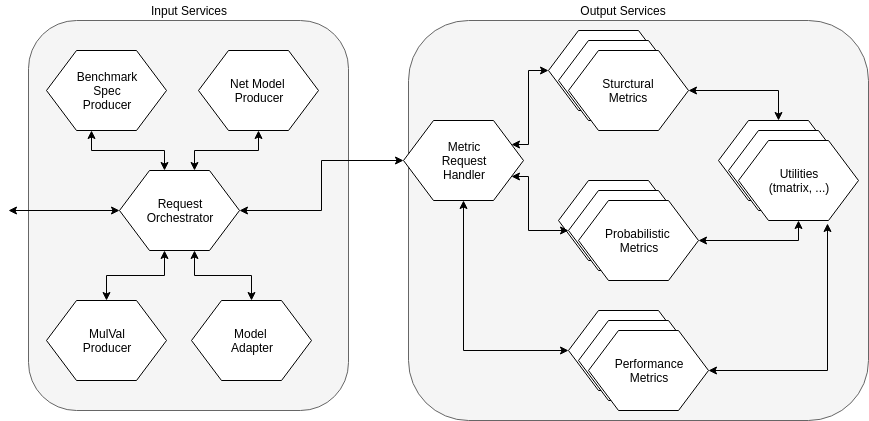
\includegraphics[width=.9\textwidth]{resource/img/ch_current/smaas/smaas_arch.png}
\caption{Security Metrics as a Service Architecture}
\label{fig:smaas:smaas_arch}
\end{figure} 


To handle the scale and volume of requests needed to support the advanced use-cases listed below, we are currently implementing and evaluating the following features in the SMaaS architecture:
Metric Isolation: Each metric should be independently deployable to allow scaling up and down as request volume dictates. Currently metrics are bundled in Python and R modules with logical separation at the function level.






\section{S-MaaS Implementation}\label{sec:smaas:impl}


One of the difficulties we encountered when trying to validate results from other papers was setting up the environment and running a test quickly. A side effect of deployment automation from Chapter \ref{ch:automation} is that we are instrumented for integration into existing DevOps pipelines. 

 

\begin{minipage}{\linewidth}
\begin{lstlisting}[language=yaml, label={lst:smaas_fnatrix}, caption={Define Multiple Tests in a Single Line},captionpos=b, linewidth=1\textwidth]
mttf:
    flag_matrix: fmatrix
    flag_matrix_defs:
        fmatrix:
            secmet_fix_cvss_score: [1, 2, 3, 4, 5, 6,  7, 8, 9, 10]
       
\end{lstlisting}
\end{minipage}





% \subsection{Dependency Graph Checking}\label{sec:smaas:dependency}




% \subsection{Deployment Considerations}\label{sec:smaas:deployment}




\begin{figure}[ht]
\centering
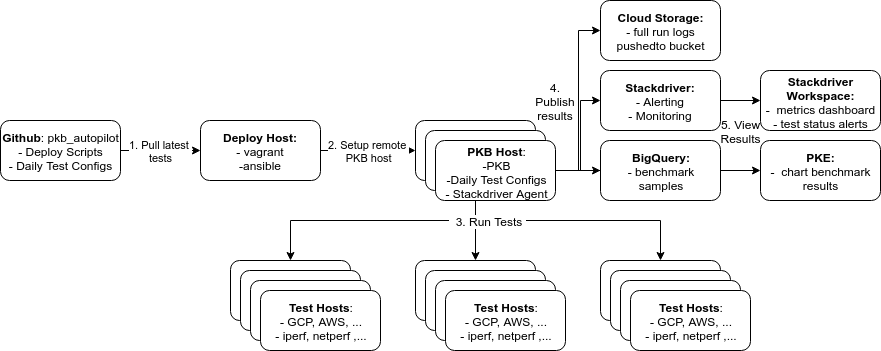
\includegraphics[width=.95\textwidth]{resource/img/ch_benchmarking/autopilot_arch.png}
\caption{S-MaaS Deployment Automation}
\label{fig:smaas:autopilot_arch}
\end{figure} 




% \subsection{Monitoring \& Alerting}\label{sec:smaas:alerting}




\begin{figure}[ht]
\centering
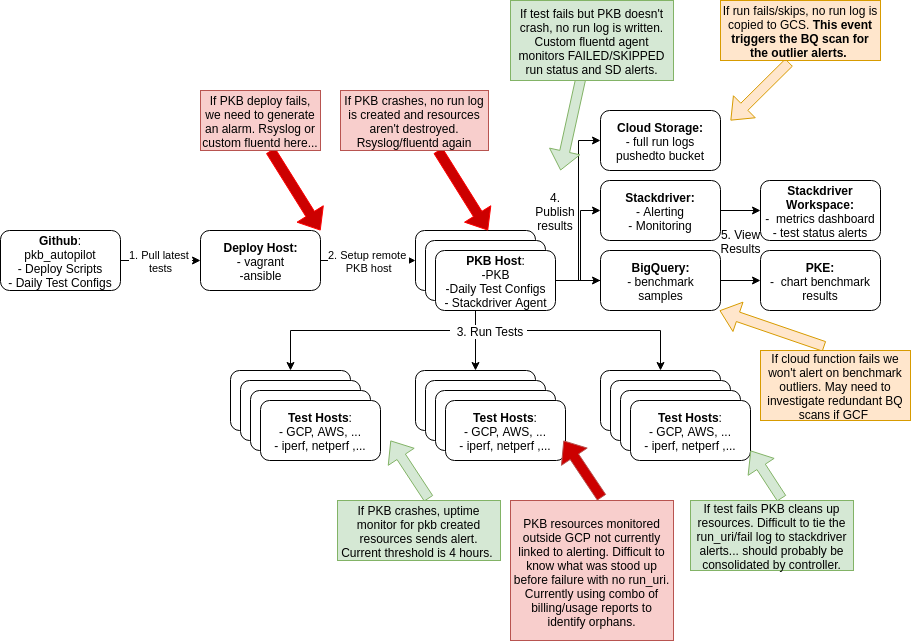
\includegraphics[width=.75\textwidth]{resource/img/ch_benchmarking/alert_points.png}
\caption{Alert Points within Automation }
\label{fig:smaas:alert_points}
\end{figure} 




\begin{minipage}{\linewidth}
\begin{lstlisting}[basicstyle=\linespread{0.5}\listingsfont, language=json, label={lst:smaas_result}, caption={Sample S-MaaS Results},captionpos=b, linewidth=1\textwidth]
{
  "metric": "MTTF",
  "value": 9.166666666666666,
  "unit": "Weeks",
  "timestamp": 1581337987.3571074,
  "test": "mttf",
  "product_name": "py_mulval",
  "official": false,
  "owner": "cat-dog",
  "run_id": null,
  "sample_uri": "91cfe225-ca65-4c0a-83ca-728d98be5779",
  "labels": "|attack_graph_name:single_host_1|, |citation:[1]Marc Dacier, Yves Deswarte, and Mohamed Ka\u00e2niche. 1996. Quantitative assessment of operational security: Models and tools. Information Systems Security, ed. by SK Katsikas and D. Gritzalis, London, Chapman & Hall (1996), 179\u201386.\n|, |cite_key:Dacier1996|, |mttf:[1.4999999999999998, 1.75, 2.6666666666666665, 3.25]|, |run_number:0|, |tmatrix_headers:[\"13\", \"8\", \"5\", \"3\", \"1\"]|, |tmatrix_probs:[[0.3333333333333333, 0.3076923076923077, 0.358974358974359, 0.0, 0.0], [0.0, 0.42857142857142855, 0.5714285714285714, 0.0, 0.0], [0.0, 0.0, 0.625, 0.375, 0.0], [0.0, 0.0, 0.0, 0.6923076923076923, 0.3076923076923077], [0.0, 0.0, 0.0, 0.0, 1.0]]|"
}
{
  "metric": "End to End Runtime",
  "value": 0.07858085632324219,
  "unit": "seconds",
  "timestamp": 1581337987.3574076,
  "test": "mttf",
  "product_name": "py_mulval",
  "official": false,
  "owner": "cat-dog",
  "run_id": null,
  "sample_uri": "c74d70cf-e783-4c40-9ec3-2ff47bbac8a0",
  "labels": ""
}
\end{lstlisting}
\end{minipage}
 \label{ch:smaas}


\chapter{Validating Security Metrics With Benchmarking}\label{ch:benchmarking}



If we measure an aspect of security before and after a change takes place, then we can quantify the impact that change had on security. If we test an aspect of cyber security at regular intervals, then we can determine the rate of change for that property over time. In order to sample security measurements at regular (approaching continuous) intervals, we assert that the test apparatus must be fully automated. The necessity of such automation is critical to evaluating security metrics in a repeatable and consistent way. 

% \begin{figure}[ht]
% \centering
% \includegraphics[width=\linewidth]{img/metric_calc_pipeline.png}
% \caption{Generalized Metric Evaluation Pipeline}
% \label{fig:automation:metric_pipeline}
% \end{figure} 

In Figure \ref{fig:automation:metric_pipeline} we present a general four-stage pipeline for security metric processing based on our observations implementing a number of metrics from the literature. This abstraction encourages us to:
\begin{itemize}
\item Decouple the source of system information from the representation of that information. 
\item Decouple the actual calculation of the metric from the input model representation it is typically paired with in its publication. 
\item Decouple the calculation logic and supporting metadata from any assumptions about how that measured value will be used in the future. 
\end{itemize}

In doing so, it becomes possible to identify shared dependencies among metrics, enables a systematic examination of the characteristics and behaviours of each metric across a range of inputs, and supports more reusable and composeable components for a greater variety of deployment scenarios. The remainder of this section provides the considerations and details of each stage.

The number of security metrics available in the literature is somewhat overwhelming. Surveys of security metrics from many\cite{Bohme_Nowey_2008, Haque_Keffeler_Atkison_2017, Hecker_2008, Kordy_2013, Kundu_Ghosh_Chokshi_Ghosh_2012, Pendleton_Garcia-Lebron_Cho_Xu_2016, Ramos_Lazar_Filho_Rodrigues_2017, Rudolph_Schwarz_2012, Savola_2007, Tavallaee_Stakhanova_Ghorbani_2010, Verendel_2009,  Wagner_Eckhoff_2015} sources and perspectives have been conducted, resulting in a multitude of taxonomies for each declaring when and where and how a metric should be applied.  What is notably lacking from these surveys, and indeed from much of the literature reviewed, is any empirical evaluation of the values measured by a given metric. The study of security metrics lacks the context needed to support adoption. What we provide in this chapter is a mechanism to establish the needed context by answering how well do these metrics perform individually across a variety of scenarios, and how do they compare with each other for a given model. To build context for security metrics, we break up our experiments into two parts. 

The first part \textit{sizes} the metric, examining how it behaves across different types and scales of input networks. We apply the metrics implemented in Section \ref{sec:automation:secmet_impl} to a set of models representative of different deployment scenarios. These models include enterprise networks and core networks at scales we label small, medium, and large. The models  act as a reference set against which we can evaluate properties of the implemented metrics. Our primary questions are how do these metrics perform as the size of the system changes, and how do they perform in different types of systems. As our reference set grows, we can develop an understanding of the fundamental or universal security properties we can measure, along with the best metrics for a specific situation. 

The second part \textit{ranges} the metric, examining how it behaves as the security of the system under test changes. We select a system model from our standard set and generate an attack model for a scenario. The range of transition values in the attack model varies by metric, but we can, in the general case, fix these values to present a minimally and maximally secure model with respect to the chosen metric. This bounds the security of a system to a specific range, and measurements within this interval characterize the behaviour of the metric for a scenario. We make observations about monotonicity and sensitivity with respect to a metric and describe properties common across metrics. 

We consider ranging and sizing as two aspects of security metric benchmarking. By benchmarking security metrics we validate their fitness for use in general scenarios, and create reference against which we can measure future security metrics. The rest of this chapter describes the design, testing, and findings from this research. 

\section{Benchmarking Background}\label{sec:benchmark:pkb_background}



% NIST 800-55\cite{Swanson_Bartol_Sabato_Hash_Graffo_2003} describes security metrics as "\textit{tools designed to facilitate decision making and improve performance and accountability through collection, analysis, and reporting of relevant performance-related data. IT security metrics must be based on IT security performance goals and objectives.}"

When system performance is described, it tends to be in quantifiable terms. The metrics chosen are well understood characteristics like network latency and disk IOPS, the measurement tools are capable of sampling the desired metrics repeatably, and the results are reported with consistency. Benchmarks can be used to compare competing alternatives against a desired metric, to evaluate the effect of changes made to an existing system, or to confirm that expected service level agreements are met. It's easy to draw a line between system performance and return on investment.

In contrast, system security discussions can be somewhat less intuitive. Common measures include compliance level, patch cycle frequency, or the number and severity of vulnerability scan findings. The CVSS\cite{Mell07thecommon} framework provides a method to score software vulnerabilities on metrics like impact or complexity, along with knobs to tune the base score according to temporal or environmental factors. Scored vulnerabilities offer a ranking method for remediation priority, but don't give insight into the system's overall security posture since each vulnerability is scored in isolation. 

Each vulnerability requires a set of preconditions to exist in order to perform an exploit successfully; if an unpatched service is running but an attacker can't connect to the listening port due to firewall rules, then the vulnerability is not reachable. When a vulnerability is exploited successfully, the resulting postconditions (escalated privileges for example) are applied to the attacker and environment, potentially opening the way to previously unreachable vulnerabilities. A common representation of the reachability between vulnerabilities in a system is a directed graph, where an edge exists between two nodes when all preconditions needed to compromise the successor are met by the predecessor. By assigning an attacker an initial set of preconditions and a set of target postconditions as the goal, then a sequence of nodes with edges connecting the initial position and the target forms an attack path, and the enumeration of all possible attack paths is the attack graph. The attack graph augmented with CVSS scores forms the basis of many of the model based security metrics described in \cite{Pendleton_Garcia-Lebron_Cho_Xu_2016}\cite{Ramos_Lazar_Filho_Rodrigues_2017}\cite{Verendel_2009} which we briefly review in Section \ref{sec:background:metrics}.

There are numerous security metrics published, but what we have encountered in practice supports Verendel's conclusions in \cite{Verendel_2009} and Pendleton's in \cite{Pendleton_Garcia-Lebron_Cho_Xu_2016} - that there is a lack of validation for many of the quantitative methods described in the literature. Attack graph based security metrics tend to be studied in isolation, with the result produced being a mathematical derivation demonstrating analytical soundness, possibly accompanied by a simple use-case to illustrate applicability. What is missing from these studies is a standard methodology and data set to verify security performance against.

% \begin{definition}
% \textbf{Metric}: The definition of a specific standard unit of measurement.
% \end{definition}
% \begin{definition}
% \textbf{Measurement}: A sampled value of a metric.
% \end{definition}
% \begin{definition}
% \textbf{Test}: The instrument and procedure used to obtain a measurement.
% \end{definition}
% \begin{definition}
% \textbf{Benchmark}: The environment and observed measurements for a test.
% \end{definition}

% Performance Benchmarking 
What we propose is a framework for measuring the relative performance of model based security metrics. Benchmarks exist for most other aspects of computing; for network, compute, and storage hardware, for machine learning, stream processing, cache serving, code compiling, and even for other areas of security like cryptographic libraries, spam filtering, and intrusion detection systems. Paxson \cite{Paxson_2004} provides generally applicable characteristics of \textit{good} benchmarks: 
\begin{itemize}
\item \textit{Precision} is a limitation of the tool's ability to measure beyond a certain level of detail.
\item \textit{Accuracy} errors are differences between the measurement we took and the actual value of the thing we measured. Paxson's example is tcpdump silently dropping packets, leading to difference between measured packet count and actual packets sent.
\item \textit{Misconception} errors are differences in what we intended to measure and what we actually measured. Several examples related to incorrect implementation of network tests (packet loss by retrans count, throughput without filling xfer size filling send buffer)
\item \textit{Calibration} is used to reduce errors in accuracy and misconception - 4 strategies including testing edge cases, consistency checks, synthetic test data, and retest with different methods to validate.
\item \textit{Metadata} should be associated with each measurement - can limit precision errors and make data re-usable
\end{itemize}

These properties must be taken into account when designing a measurement instrument for our metric validation framework. Preventing misconceptions about what we are measuring is of particular importance, as the measurement units of many security metrics are not particularly intuitive. 



% Measurements need units, and they also need context. We can measure the top speed of a specific car model, but we can't say that car is \textit{fast} unless we compare our measurement to other cars. We can say that a car is not fast compared to the speed of light, but there isn't much value in that statement. Similarly, 



% Security Benchmarking: 


% \section{Performance Benchmarking}\label{sec:benchmark:pkb}

% 

PerfKit Benchmarker is an open source tool originally created at Google that allows users to easily run benchmarks on various cloud providers without having to manually set up the infrastructure required for those benchmarks. PerfKit Benchmarker follows the 5 step process detailed in Figure 1 to automate each benchmark run. The Configuration phase processes command line flags, configuration files, and benchmark defaults to establish the final specification used for the run. The Provisioning phase creates the networks, subnets, firewalls and firewall rules, virtual machines, drives, and other cloud resources required to run the test. Benchmark binaries and dependencies like datasets are also loaded in this phase. The Execution phase is responsible for running the benchmarks themselves,  and Teardown releases any resources created during the Provision phase. The Publishing phase packages the test results into a format suitable for further analysis such as  loading into a reporting system. The metadata returned from the Publishing phase can include verbose details about the actual infrastructure used during the test and timing information for each phase of the run along with the metrics returned from the benchmark itself, providing the level of detail needed to understand the benchmark results in context.


\begin{figure}[ht]
\centering
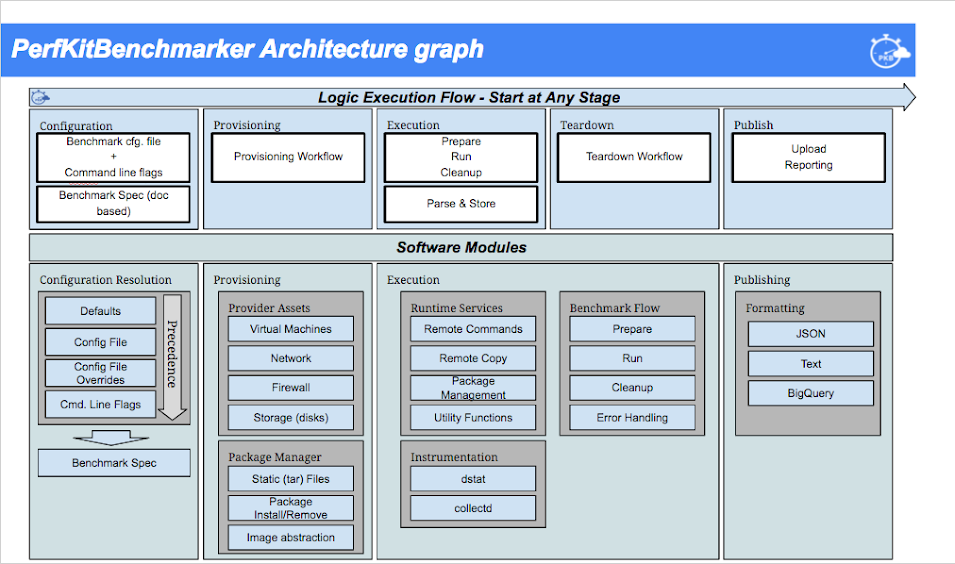
\includegraphics[width=.75\textwidth]{resource/img/ch_benchmarking/pkb_arch.png}
\caption{Perfkit Benchmarker Run Stage Breakdown}
\label{fig:benchmarking:pkb_arch}
\end{figure} 


\section{Security Benchmarking}\label{sec:benhmark:sec-pkb}




While we primarily focus on model based security metrics in this work, at a high level all security metrics follow the simplified processing pipeline shown in Figure \ref{fig:benchmarking:metric_pipeline}. In order to automate this process, significant effort is involved in preparing the input data and packaging the output in a way that can be applied to all metrics.

% Table \ref{tab:metric_proc_pipeline}. 

% \begin{table}[ht]
% \centering
% \caption{Generalized Metric Pipeline}
% \label{tab:metric_proc_pipeline}
% \resizebox{.98\textwidth}{!}{%
% \begin{tabular}{@{}p{.20\linewidth}p{.22\linewidth}p{.22\linewidth}p{.22\linewidth}@{}}
% \toprule
%  1. Input & 2. Pre-Process & 3. Compute  & 4. Report \\ \midrule
%  System Model & Generate AG & Measurement &  Return values \\
% \bottomrule
% \end{tabular}
% }
% \end{table}

\begin{figure}[ht]
\centering
\includegraphics[width=.95\textwidth]{resource/img/ch_benchmarking/metric_calc_pipeline.png}
\caption{Generalized Metric Calculation Pipeline}
\label{fig:benchmarking:metric_pipeline}
\end{figure} 

In Step 1, the inputs include host definitions, accounts and permissions, network connectivity and ACLs, system policies, vulnerability definitions, etc. It is usually assumed these parameters are collected through standard management tools and translated into a common system model for consumption by the attack graph generation engine, although static or synthetic inputs are valuable for validating and reproducing results. 

In Step 2, the system model is examined for policy violations or possible exploits that would lead to a given target's compromise. If a compromise is possible, an attack graph is produced. This is the expected input for most of the metrics we have examined, although some also assume the edges have been weighted with CVSS scores first.

The algorithm for computing the metric is run in step 3 with the attack graph as input, and the computed result is returned in the final step. 

Our first observation is that survivorship bias\cite{Wald_1980} is implicit in all AG based security metrics. An attack graph is produced \textit{only} when a system model includes in its definition enough detail to identify possible attacks. An attack graph will \textbf{not} be created if a system is totally \textit{secure}. Secure and insecure systems should, in theory at least, be mutually exclusive and collectively exhaustive; unfortunately, an attack graph will also \textbf{not} be created if a system is totally \textit{insecure}, but the system model or processing logic is incomplete. So, when validating AG metrics, we must have accepted a priori the selection bias inherent with their use. That is, we are not measuring if a system is secure or not; rather, we are measuring just how insecure that system is. 

With this in mind, validation can be seen as a test of how well a metric captures the scale of insecurity which is known to be on the system under test. We propose here a simple methodology for calibrating a metric and gauging it's accuracy in a controlled manner. 

\begin{algorithm}
\caption{Calibrate Weighted Security Metric}
\label{alg:calibrate_secmet}
\begin{algorithmic}
\REQUIRE Valid Attack Graph, N = \# partitions
\FOR{n $\in$ range (1..N)} 
 \STATE Fix all weights at $\frac{scale}{n}$ 
 \STATE Take measurement
\ENDFOR
 \end{algorithmic}
\end{algorithm}

What we assume in Algorithm \ref{alg:calibrate_secmet} is that the security metric is using some weighting scheme to influence an attacker's selection of paths, which is common in all but the structural metrics  we've encountered. So, for CVSS base score weighted AG metrics, we would fix all vulnerabilities at the lowest score (0 or 1 in this case) and calculate the metric, and do the same again fixing all vulnerabilities at the highest score for the scale (10 for CVSS). This bounds the range of the metric under test. Creating more than 2 partitions of the score range gives us insight into the behaviour of the metric for this particular attack graph. An example of this calibration is given in \ref{ch:case_studies}

To turn this testing algorithm into a benchmark, we need attack graphs which represent typical deployment scenarios. By far the most common use cases in the literature are small enterprise systems consisting of a limited number of distinct node types (web server, database, firewall, workstation, ...) and a 2-dimensional perimeter. While these examples are easily digestible when describing the applicability of an intensive mathematical derivation, they fall short of validating the new metric as it would be seen in the wild. We propose a standard benchmark set of attack graphs which isolate interesting attack patterns for study. In this way we can target \textit{micro-benchmarks} for specific properties, and integrate or compose models for a more rounded workload examination.

\begin{table*}[ht]
\centering
\caption{AG Standard Set - Target Scenarios}
\label{tab:ag_standard_set}
\begin{tabular}{@{}p{.15\linewidth}p{.15\linewidth}p{.15\linewidth}p{.15\linewidth}p{.15\linewidth}@{}}
\toprule
 & Enterprise & MEC/MANET &  Core &  Cloud \\ \midrule
Small (10-20) & Multi Site & UE Access  & Attachment Point & API misuse \\
Medium (100-200) & Container/K8s & 4G/5G & Layer 1\&2 & Hypervisor  \\
Large (1000-2000) & Insider/Exfil  &  IoT &  SDN/NFV & APT  \\ \bottomrule
\end{tabular}
\end{table*}



\section{Benchmark Automation}\label{sec:benchmark:secperfkit}



We refer again to the system performance benchmarking analogy to describe the design considerations and methodology used in the proposed security benchmarking framework. In the performance benchmarking scenario, assume we are considering migrating from a corporate data center to the public cloud, and we want to estimate operating cost for multiple CSPs to base the comparison. Our strategy might begin by characterizing our data center's compute, network, and storage profiles and reproducing them on each of the candidate CSPs.  We can size the environments across CSPs by holding the workload parameters constant and tuning each cloud deployment until it  matches the expected baseline performance. Once we have established comparable deployment environments between clouds, we can then run the synthetic workload for the same duration on each provider and compare the costs incurred directly. After migration, benchmark tests can be scheduled to ensure SLAs are met and to inform system baseline heuristics and continuous monitoring systems. 

If we re-imagine this situation in terms of security metrics, the components needed for validation and verification begin to emerge. In this context, we are still comparing CSPs for cost efficiency, but the constraint is now to maintain the same security posture as our current system. 

The first step above was to establish the baseline performance metrics we intend to target on the systems under test. Obviously the target environments would be adjusted to account for differences in requirements - network latency and throughput might deviate based on proximity to the nearest cloud regional data center, or block storage capacity requirements might decrease given the availability of alternate cold storage services. 

Similarly, we can take a snapshot of the current security baseline by measuring any or all security metrics for the current state. This involves generating attack graphs and running simulations, or just interrogating the SIEM or other source of aggregated security telemetry for the current patch levels and AV signatures. After establishing the current baseline, we proceed with tuning the remote environments to match the baseline. This might involve scaling instance sizes to align with compute or network objectives, while tuning for security could lead to rewriting boundary service ACLs to meet the baseline attack surface target. When we tune the candidate environments to match the baseline, we are effectively calibrating our metrics for the current evaluation. After tuning is complete, running the synthetic workload (comprising network traffic generators, endpoint stressers, or disk/CPU/DB/etc relevant operation mixes for example) for a fixed amount of time should yield nearly the same results across all tuned metrics, with the exception being cost, which is the measurement we wanted to take.

\begin{figure}[ht]
\centering
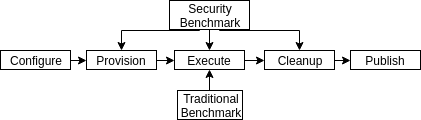
\includegraphics[width=.75\textwidth]{resource/img/ch_benchmarking/cloud_benchmarking_methodology.png}
\caption{Integrated Security Benchmarking Process}
\label{fig:benchmarking:boromir_arch}
\end{figure} 

To eliminate friction with evaluation and increase likelihood of adoption we have implemented our security benchmarks as an extension of the open source toolkit \textit{PerfKit Benchmarker}\cite{zaber_pkb}. PKB allows users to easily run benchmarks on various cloud providers without having to manually set up the infrastructure required for those benchmarks. PerfKit Benchmarker follows the 5 step process shown in Figure \ref{fig:benchmarking:boromir_arch} to automate each benchmark run. The Configuration phase processes command line flags, configuration files, and benchmark defaults to establish the final specification used for the run. The Provisioning phase creates the networks, subnets, firewalls and firewall rules, virtual machines, drives, and other cloud resources required to run the test. Benchmark binaries and dependencies like datasets are also loaded in this phase. The Execution phase is responsible for running the benchmarks themselves, and Teardown releases any resources created during the Provision phase. The Publishing phase packages the test results into a format suitable for further analysis such as  loading into a reporting system. The metadata returned from the Publishing phase can include verbose details about the actual infrastructure used during the test and timing information for each phase of the run along with the metrics returned from the benchmark itself, providing the level of detail needed to understand the benchmark results in context. 


% \begin{figure}[ht]
% \centering
% 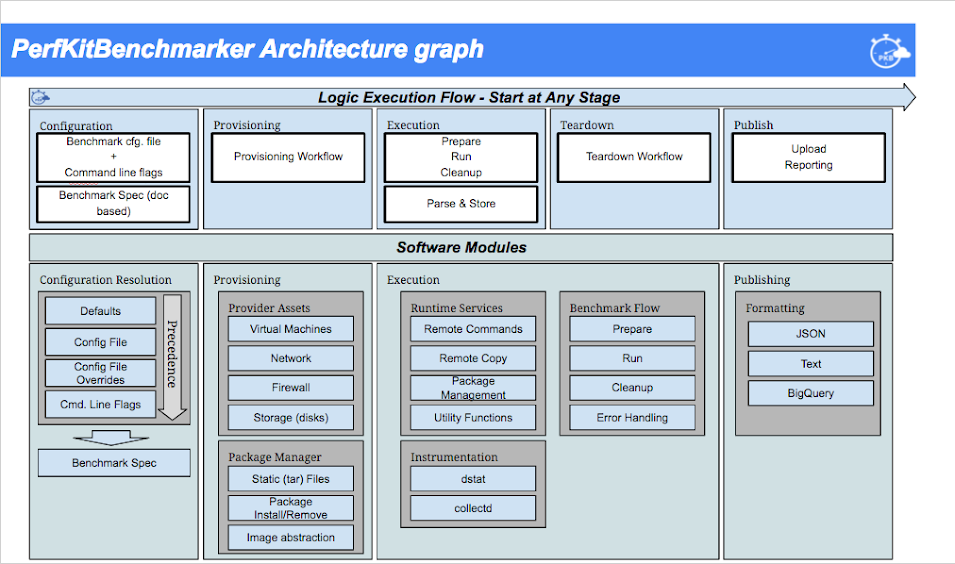
\includegraphics[width=.75\textwidth]{resource/img/ch_benchmarking/pkb_arch.png}
% \caption{Perfkit Benchmarker Run Stage Breakdown}
% \label{fig:benchmarking:pkb_arch}
% \end{figure} 


% \section{Monitoring \& Alerting}\label{sec:benhmark:alerting}

% 




 %\label{ch:benchmarking}



\chapter{Applications of Machine Learning to Security Metrics Research}\label{ch:ml}




In this chapter we investigate how machine learning can be used in conjunction with the metrics and measurements we are surfacing to improve our understanding of cyber security. 

% Specifically, we focus on the following 3 areas in this paper:
 
% \begin{enumerate}
% \item \textbf{Learning valid security metrics}: Can we apply graph clustering and similarity methods to group models by valid cyber security properties?
% \item \textbf{Model Scoring for Network Design Support}: Can we make use of existing system and threat models, along with associated security metrics, to better model attacker behavior and improve incident response? 

% \item \textbf{Vulnerability Score Fuzzing to predict metric}: Given a network model, can we predict the values of specific security metrics through classification or regression? 
% \end{enumerate}


In the December 2019 workshop\textit{ Implications of Artificial Intelligence for Cybersecurity}\cite{Chang_2019}, one of the key takeaways identified was the need to expand the connections between cyber security and applications of artificial intelligence and machine learning. In this work we have so far focused on making cyber security measurable, focusing on instrumentation for automation and autonomy. Programmatic access to security metrics through automation opens up a wide variety of applications involving, and can itself be improved by, current techniques in machine learning. In this chapter we describe the design details for the experiments we are conducting using the SMaaS environment. While adversarial AI and attacks on ML models are areas of concern today, the direction of this work is \textit{not} in applying SMaaS to evaluate the security of machine learning. Instead, we propose to investigate the use of specific machine learning techniques to improve cyber security through the metrics framework we developed above. 


\section{Machine Learning Background}\label{sec:ml:background}


Machine learning techniques can be broadly grouped into 4 categories based on the types of problems they solve. \textbf{Clustering} problems try to find groupings in data sets by minimizing distances from members of the same group and maximizing distances between members of differing groups. \textbf{Classification} problems map new instance data onto a discrete set of values representing categories or labels, while \textbf{regression} maps new data onto a continuous set of values. \textbf{Rule extraction}\cite{Denker} is a statistical inference method used to predict responses from given input patterns. It is also common to describe machine learning by one of four types of learning used. \textbf{Supervised} learning is provided labeled training data to build models from, while \textbf{unsupervised} learning is trained on unlabeled data. \textbf{Semi-supervised} learning is used with a mix of labeled and unlabeled data. \textbf{Reinforcement} learning\cite{Sutton_Barto_2018} maximizes values from an internal scoring functions to learn a model about the environment. 

The use of machine learning techniques in cyber security is just starting to be explored. The two surveys\cite{Buczak_Guven_2016, Xin_Kong_Liu_Chen_Li_Zhu_Gao_Hou_Wang_2018} published in 2016 and 2018 review a wide range of ML and RL methods specific to the area of intrusion detection. In \cite{Boutaba_2018} the authors survey the field of networking generally for uses of machine learning. Their findings cover areas in traffic management like routing and congestion control, as well as resource and fault management topics. On the subject of network security, the subject areas reviewed were again narrowly focused on intrusion detection. 

In this work we describe methods for evaluating cyber security that incorporate the underlying structure of the (computer) network under test. Graphs are a natural way to represent network connections and the relationships between system components, but preserving that structure adds complexity to the cost of analysis. Modern machine learning techniques make use of optimizations and transformations to reduce their complexity, and graph learning methods are no exception. Similar to preprocessing an image set to uniform dimensions prior to training, many graph learning methods presuppose an embedding of the graph data as input requirement. Goyal’s graph embedding survey\cite{Goyal_Ferrara_2018} finds 4 broad categories of these methods:
\begin{enumerate}
\item \textbf{Node Classification}: Predict the label of a node based on its embedding. 
\item \textbf{Link Predicton}: Predict edge based on embeddings of nodes it joins.
\item \textbf{Clustering}: Community detections and node groupings.
\item \textbf{Visualization}: Interpreting more than a few dozen nodes becomes difficult. 
\end{enumerate}

Graph embedding can mean either embedding the entire graph in vector space, or embedding each node in vector space. The goal in either case is to encode the graph data onto a lower dimensional space while retaining the relevant structural relationships. Common practice is to learn graph embeddings by defining the encoding and similarity functions, and then optimize the encoding parameters which maximize the similarity. How the similarity distance is measured and which properties are selected for feature encoding are some of the challenges in deciding the best embedding method\cite{Goyal_Ferrara_2018}. 

% For a graph $G=(V,E)$, a node embedding function $f:u\rightarrow\mathbb{R}^n$ maps each node $u \in G$ onto a $d$ dimensional set of real values called a feature vector. For any two nodes $u,v\in G$, a similarity function $sim(u,v)$ measures the strength of the relationship between the two nodes. Because nodes can be related in many different ways, there are multiple ways to measure similarity. The proximity of the encoded nodes in the embedding space reflects the similarity of the nodes in the original graph. Current embedding approaches include matrix factorization\cite{belkin2002laplacian}\cite{ahmed2013distributed}, random walks\cite{perozzi2014deepwalk}\cite{grover2016node2vec} and deep learning\cite{wang2016structural}\cite{kipf2016semi}

% \cite{Kutuzov_Dorgham_Oliynyk_Biemann_Panchenko_2019}

% \cite{Hamilton_Ying_Leskovec}

% \begin{figure}[ht]
% \centering
% \includegraphics[width=\linewidth]{resource/img/ch_benchmarking/metric_calc_pipeline.png}
% \caption{Generalized Metric Evaluation Pipeline}
% \label{fig:automation:metric_pipeline}
% \end{figure} 


\section{Problem Identification and Approach}\label{sec:ml:approach}



% \section{Experiments}\label{sec:approach}
\input{content/chapters/ch_ml/approach/main}



\subsection{Data Generation and Representation}
\label{ml:approach:subsec1}
\input{content/chapters/ch_ml/approach/subsec1}

\subsection{Preperation for Standard ML Pipelines}
\label{ml:approach:subsec2}
\input{content/chapters/ch_ml/approach/subsec2}


\section{Experiments and Results}\label{sec:ml:exp_results}



% \section{Experiments}\label{sec:approach}
% \input{content/chapters/ch_ml/approach/main}

% \section{Results}\label{sec_results}
\input{content/chapters/ch_ml/results/main.tex}

% \subsection{Initial Classification Attempts and Problem Identification}
\input{content/chapters/ch_ml/results/subsec1.tex}

% \subsection{Feature Engineering and Clustering}\label{results_subsec_data_mmung}
\input{content/chapters/ch_ml/results/subsec2.tex}

% \subsection{Embeddings - Words, Nodes, and Graphs to Vec}\label{results:subsec3_embedding}
\input{content/chapters/ch_ml/results/subsec3.tex}
 

% \subsection{Similarity Measures for Graph Classification }\label{results:subsec4_similarity}
\input{content/chapters/ch_ml/results/subsec4.tex}


% \subsection{Feature Engineering, Target Clustering}\label{results:subsec5_embedding}
% \input{content/chapters/ch_ml/results/subsec5.tex}

% \subsection{Feature Engineering, Target Clustering}\label{results:subsec4_embedding}
% \input{content/chapters/ch_ml/results/subsec6.tex}

\section{Discussion of Findings}\label{sec:ml:discussion}



In the literature we reviewed there were over 500 distinct security metrics identified. The surveys each provided their own classification systems which were appropriate for the analysis they conducted, but none of these taxonomies generalize well to classify all types of security metrics. We describe properties common to all metrics, identify overlaps in the various taxonomies, identify points of confusion between existing metric hierarchies, and describe a suitable and intuitive system for classifying any current or future security metric. In using the CyBOK as the underlying classification system we are also able to determine the distribution of metrics in each topic and identify areas of limited coverage which would benefit from future research. 

In reproducing the results from the literature, we faced several issues during implementation, particularly with model based security metrics. Often assumptions were made about the intermediate processing of the pipeline that weren't surfaced in the supporting examples of the publication. We note that many of the survey authors describe security metric validation as an area of concern in security metric research. In response to these concerns and to move forward in our own research, we identified a generalized four step processing pipeline that separates the core steps of this process. By following this workflow we have identified and implemented many reusable preprocessing components, allowing us to rapidly add new security metrics from the literature and immediately test the performance of those metrics against a growing number of input models we use as our reference set. 

By enforcing the 4 stage pipeline abstraction, we achieve several benefits. Each phase is modular so that replacing any piece in the pipeline is straight forward. By plugging in the static reference set to the input phase we create a \textit{unit test} of sorts for our metric library, SecMet. With PTaH, the preprocessing and transformation handlers described above, we can articulate how any or all of the security metrics will behave under a variety of conditions for any given input - not just the reference set we describe above. This, in theory at least, should make characterizing the behaviours of security metrics on internal or sensitive systems as simple as adding input adapters to the existing set, which already includes Nessus, OVAL, NVD, CVE, and now SSFNet. By replacing our validation PTaH with whatever workflow execution engine is already in place, Apache Beam or Storm for example, the SecMet catalog becomes a drop in security measurement aid to support SecDevOps which we refer to as Security Metrics as a Service (S-MaaS).

Our takeaways from the experiments described above indicate that, while validating security metrics is not done rigorously in many of the publications, a mechanism for validation and analysis is not out of reach. By streamlining the development and evaluation process with automation, we aim to lower the barrier to entry in the field and allow researchers to spend more time developing and analyzing security metrics, which in turn should encourage more secure systems being deployed. 



 %\label{ch:benchmarking}


\chapter{Case Study} \label{ch:case_studies}

\section{Carrier Network Migration}\label{sec:case_studies:att}

We consider the use case of a network operator migrating core infrastructure from traditional switching and routing elements to a centrally managed SDN architecture. We assume the migration process will occur in three discrete phases, with a single intermediate migration state. 


% \section{Application Case Study:}\label{subsec:approach:main}
% \input{content/approach/main.tex}

\subsection{Migration Path}
\input{content/chapters/ch_case_studies/att/input_model}


\subsection{Vulnerabilities}
\input{content/chapters/ch_case_studies/att/vulns}


\subsection{Results}
\input{content/chapters/ch_case_studies/att/results}


\subsection{Conclusions}
\input{content/chapters/ch_case_studies/att/conclusions}


% \subsection{Input Network and System Modeling}\label{subsec:approach:model}
% \input{content/approach/input_model.tex}

% \subsection{Ports, Protocols, and Services}\label{subsec:approach:ppp}
% \input{content/approach/ppp.tex}

% \subsection{Vulnerabilities}\label{subsec:approach:vulns}
% \input{content/approach/vulns.tex}

% \section{Secure Stream Processing}\label{sec:case_studies:stormcellar}
 %\label{ch:case_studies}

% \part{Ongoing Work}\label{part:future}

\chapter{Future Work} \label{ch:future}
% \section{Applicatons in ML} \label{sec:ml} 
% In the December 2019 workshop\textit{ Implications of Artificial Intelligence for Cybersecurity}\cite{Evans_2008}, one of the key takeaways identified was the need to expand the connections between cyber security and applications of artificial intelligence and machine learning. In this work we have so far focused on making cyber security measurable, focusing on instrumentation for automation and autonomy. Programmatic access to security metrics through automation opens up a wide variety of applications involving, and can itself be improved by, current techniques in machine learning. In this section we describe the design details for the experiments we are developing using the SMaaS environment. While adversarial AI and attacks on ML models are areas of concern today, the direction of this work is \textit{not} in applying SMaaS to evaluate the security of machine learning. Instead, we propose to investigate the use of specific machine learning techniques to improve cyber security through the metrics framework we developed above. 

% Machine learning techniques can be described by the 4 key types of of problems they solve. \textbf{Clustering} problems try to find groupings in data sets by minimizing distances from members of the same group and maximizing distances between members of differing groups. \textbf{Classification} problems map new instance data onto a discrete set of values representing categories or labels, while \textbf{regression} maps new data onto a continuous set of values. \textbf{Rule extraction}\cite{Denker} is a statistical 
% inference method used to predict responses from given input patterns. 

% It is also common to describe machine learning by one of four types of learning used. \textbf{Supervised} learning is provided labeled training data to build models from, while \textbf{unsupervised} learning is trained on unlabeled data. \textbf{Semi-supervised} learning is used with a mix of labeled and unlabeled data. \textbf{Reinforcement} learning\cite{Sutton_Barto_2018} maximizes values from an internal scoring functions to learn a model about the environment. 

% Machine learning is a fast moving research area. We consult the 2019 \textit{Deep Learning in Mobile and Wireless Networking: A Survey}, \cite{Zhang_Patras_Haddadi_2019}, 2018 \textit{A comprehensive survey on machine
% learning for networking}\cite{Boutaba_2018}, and the 2018 \textit{Machine Learning and Deep Learning Methods for Cybersecurity}\cite{Xin_Kong_Liu_Chen_Li_Zhu_Gao_Hou_Wang_2018} to identify current techniques and canonical literature for our topic. 

% MulVal Facts : Datalog facts defining system model: (Hosts, Policies, Principals, Vulnerabilities, Interaction Rules) + (Attacker Location, Goal)
% MulVal Output: DAG of possible paths attacker can reach goal (nxn connectivity matrix)

% \section{Security Metric Prediction}

% Problem Type: Classification and Regression problem.

% There are quite a few scenarios that can be described as ‘Metric Prediction’. In general we approach these as supervised categorical classification or regression tasks, where SMaaS is used to create a labeled dataset of network models or attack graphs with the resulting security metric(s). Training and validation proceed as usual, with the resulting model able to predict the metric of new network states or topologies without needing the SMaaS system.

% 1a. Vulnerability Score Perturbation to predict metric


% \begin{figure}[ht]
% \centering
% 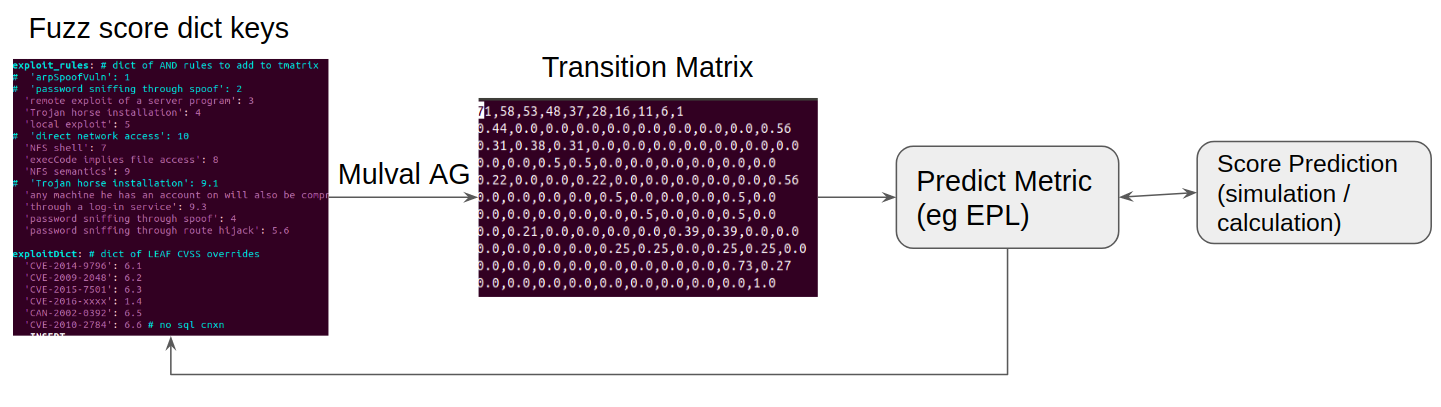
\includegraphics[width=.9\textwidth]{resource/img/ch_future/1a.png}
% \caption{Learning Metrics from Vulnerability Score}
% \label{fig:final:1a}
% \end{figure} 

% Goal: Given a weighted transition matrix $\longrightarrow$ predict specific metric

% Method: Fuzz vulnerability weights (won't affect AG structure)
% \begin{itemize}
% \item Find best fit function (LR, …)
% \item Compare time/perf over simulation for small/med/large matrixes
% \item Compare performance for different metrics (within/outside same class)
% \item Fuzz subset of vulns for PCA or confuse
% \end{itemize}

% 1b. Vulnerability Placement Fuzzing 

% \begin{figure}[ht]
% \centering
% 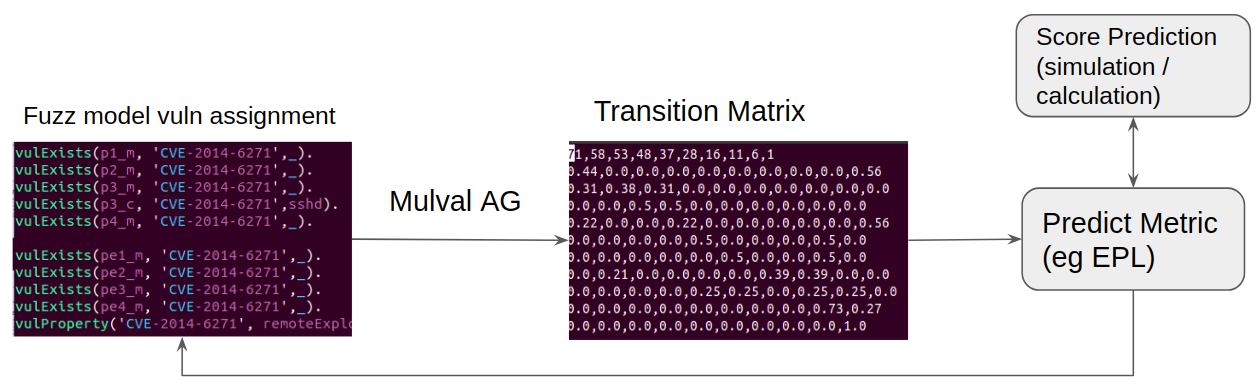
\includegraphics[width=.9\textwidth]{resource/img/ch_future/1b.png}
% \caption{Learning Metrics from Vulnerability Placement}
% \label{fig:final:1b}
% \end{figure} 

% Goal: Given a MulVal model $\longrightarrow$ predict specific metric

% Method: Fuzz vulnerability placements (will affect AG structure)

% \begin{itemize}
% \item Can we learn if an AG will be produced (connectedness)?
% \item Can we predict any metrics?
% \item Might be a good application for GNNs 
% \item Could either learn on tmatrix (easy) or MulVal model (harder)
% \end{itemize}




% 1c. Network Model Fuzzing 


% \begin{figure}[ht]
% \centering
% 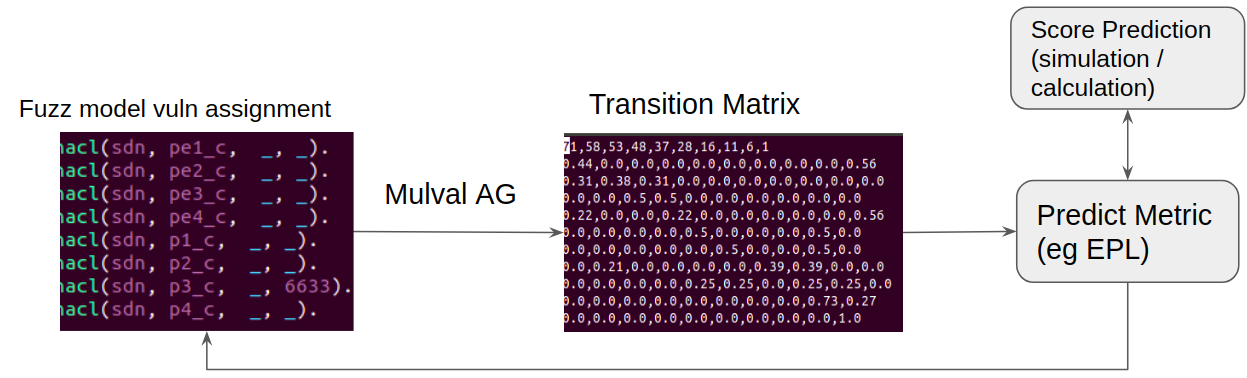
\includegraphics[width=.9\textwidth]{resource/img/ch_future/1c.png}
% \caption{Learning Metrics from Network Topology}
% \label{fig:final:1c}
% \end{figure} 


% Goal: Given a MulVal model $\longrightarrow$ predict specific metric

% Method: Fuzz network facts (will affect AG structure)
% \begin{itemize}
% \item Can we learn if an AG will be produced (connectedness)?
% \item Can we learn how to make a valid Network model?
% \item Prolog syntax/token understanding needed
% \end{itemize}


% \section{Model Enhancements}

% The reliability of a measurement depends on the reliability of the input. \textit{Garbage in, garbage out} is especially true for model based calculations. In Section \ref{sec:automation:infra} we discussed the role \textit{interaction rules} play in defining the possible attacks against a system, and that a model missing relevant interaction rules will falsely report no possible attacks when, in fact, they do exist. 

% In order to ensure complete coverage of IRs for the domains we model, we need to have these rules defined systematically. A good starting point is MITRE's CAPEC\cite{Corporation}, the Common Attack Pattern Enumeration and Classification dataset. While this corpus includes primarily application type attacks, another dataset, CyBOX (recently moved into STIX), includes attack patterns observable at lower layers like infrastructure and physical such as those we defined in Section \ref{sec:automation:infra}.  
% Recall from Section \ref{sec:background:modeling} that an interaction rule can be represented as a \textit{Horn Clause} of the form $A\xleftarrow[]{} B_1, B_2,\dots, B_n $, where $B_1, B_2,\dots, B_n $ are facts defining preconditions that must be true to assert $A$ is true. Both CAPEC and CyBOX include preconditions with each attack pattern, but sadly they chose to make this field free text and not categorical. Noel in \cite{Noel_2018} describes text mining techniques for many scenarios but prerequisite enumeration is not one of them. 

% \begin{verbatim}
% This attack requires the following:
% 1. The application uses environment variables.
% 2. An environment variable exposed to the user is vulnerable to a buffer overflow.
% 3. The vulnerable environment variable uses untrusted data.
% 4. Tainted data used in the environment variables is not properly validated. 
% \end{verbatim}

% The example above lists the CAPEC preconditions for the \textit{authentication abuse, ID:114} attack pattern. There are currently 517 unique attack patterns, along with associated prerequisites and \textit{consequences}, which capture post conditions like privileges gained from a successful attack. Our goal in this work is to expand the knowledge base for threat model generation to more accurately represent known patterns, and to accommodate future patterns as they become known.

% \subsection{Interaction Rule Mining}


% Problem Type: Association Rule Learning


% \begin{figure}[ht]
% \centering
% \includegraphics[width=.9\textwidth]{resource/img/ch_future/rule_learning.png}
% \caption{Association Rule Learning}
% \label{fig:final:learn_rule}
% \end{figure} 

% Goal: Given a Network model $\longrightarrow$ learn vulnerability rules and conditions
% \begin{itemize}
% \item Need fine grained data (ports/protocols/services/versions)
% \item Can we learn conditions for existing exploits?
% \item Can we learn conditions for new exploits?
% \item Output needs to comply with datalog AST (need ANTL/Thrift here maybe)
% \end{itemize}

% At the heart of MulVal is the interaction rule, which describes how each the set of facts combine to derive new information about the system. These derived facts then describe how attackers can advance through the system towards a target. Developing interaction rules is currently an artistic endeavor undertaken by a subject matter expert… that is to say, it is error prone, and MulVal includes around 30 interaction rules to derive the following 8 facts:

% \begin{lstlisting}[style=datalog, label={lst:fut:facts}, caption={Mulval Derived Facts}]
% derived(accessFile(_machine,_access,_filepath)).
% derived(accessMaliciousInput(_host, _principal, _program)).
% derived(canAccessHost(_host)).
% derived(dos(_host)).
% derived(execCode(_host, _user)).
% derived(logInService(_host, _protocol, _port)).
% derived(netAccess(_machine,_protocol,_port)).
% derived(principalCompromised(_victim)).
% \end{lstlisting}
% As we have demonstrated previously, the existing MulVal model leaves large gaps in defining the entire attack surface of a network. To begin covering the possible IR set it will be necessary to automate the rule generation process.
% %The path forward in this area is outlined in Table \ref{tab:future_work:rule_learning} 

% \begin{itemize}
% \item Map existing actively maintained taxonomies like MITRE’s CAPEC (common attack patterns), STIX (structured threat information), or MAEC (malware attribute enumerations) to an ontology of simple subject-verb-object relations.
% \item Translate this ontology into DataLog Horne clauses
% \item Translate the populated taxonomy information to DataLog Facts
% \item Use these IR rules to seed the next phase of ML or RL based rule learners and rule refiners \cite{Mohamed_Salleh_Omar_2012, Hahsler_Chelluboina}
% \item Evaluate the efficacy of the ML rule learners by comparing to established attack patterns (withhold a subset of MITRE rules for testing, validate new rules not in test set through penetration test)
% \end{itemize}


% % \section{Network Model Generation}

% % Problem Type: Auto Encoder / LSTM


% \subsection{Agent Based IR Learning}

% Problem Type: Reinforcement Learning

% Goal: Demonstrate the feasibility of using RL to model attacks. Further, identify if and when security metrics are appropriate to incorporate into the environment responses, agent value function, or agent policy to model attacker or defender behaviour. 

% Reinforcement learning\cite{Sutton_Barto_2018} is a computational method of building an optimal set of interactions between an agent and its environment to achieve a specific goal. A \textit{policy} defines the agent's behaviour for a given environment state. A \textit{reward signal} defines the goal as a single reward value returned at each time step. A \textit{value function} is used to predict the maximum reward available to the agent in the given environment. Environment state can be described using a Markov decision process similar to how we have already modeled attacker state in some of our metrics. 

% \textit{Model-free} RL can be thought of as trial and error based learning, where the agent doesn't need to understand how its actions affect the environment. In model-free RL, Q-learning is the most well studied and widely used method\cite{Boutaba_2018}. 

% \textit{Model-based} RL allows an agent to make inferences about how the environment will behave by planning how possible actions will change the environment's state. The simple tic-tac-toe example given by \cite{Sutton_Barto_2018} uses the 3x3 board as a model which can be used by an agent to anticipate the results of potential moves and plan for an optimal strategy against an opponent. 

% In our case, we already have two distinct models for this type of reinforcement learning. The first model is the 'normal use' transition matrix of the system model that shows connectivity between elements given as a set of user and system principals and permissions, network ports and protocols, and access control lists. The second model is the transition matrix of the exploitable paths in the resulting attack graph.    

% \section{Applicatons in the SOC} \label{sec:soc} 
% \section{Applicatons in SDN} \label{sec:sdn} 


 %\label{ch:future}


% \chapter{Conclusions \& Timeline} \label{ch:conclusion}

\input{content/chapters/ch_conclusion/conclusion_intro}


\section{Conclusions \& Future Work}\label{sec:conclusion:conclusion}


System security metrics are valuable only if they can produce timely, actionable measurements. In this thesis we have demonstrated a path forward for developing, testing, validating, and integrating security metrics into the full life cycle of a system. 

In Chapter \ref{ch:background} we present the current state of security metrics. We list the working taxonomies that these metrics can be categorized by, and elaborate on the distinctions that lead to confusion when discussing security measurements. We then review modeling techniques and how these models can isolate the security properties of a system we intend to measure. 

Chapter \ref{ch:automation} presents our unified framework for security measurement and analysis, including the model for implementing individual metrics and the infrastructure built around these metrics to drive automation in a variety of scenarios. Here we establish the security metric inheritance hierarchy and enumerate properties common to all metric types and those specific to each metric subtype. We provide our extensions to attack models that expand the range of systems that can be represented. We describe how we implemented automation from the view points of a security researcher or measurement analyst, and develop our concept of security metrics as a service, \textit{S-MaaS}, with considerations for deployment in a continuous integration or stream processing environment.

% By enforcing the 4 stage pipeline abstraction, we achieve several benefits. Each phase is modular so that replacing any piece in the pipeline is straight forward. By plugging in the static reference set to the input phase we create a \textit{unit test} of sorts for our metric library, SecMet. With PTaH, the preprocessing and transformation handlers described above, we can articulate how any or all of the security metrics will behave under a variety of conditions for any given input - not just the reference set we describe above. This, in theory at least, should make characterizing the behaviours of security metrics on internal or sensitive systems as simple as adding input adapters to the existing set, which already includes Nessus, OVAL, NVD, CVE, and now SSFNet. By replacing our validation PTaH with whatever workflow execution engine is already in place, Apache Beam or Storm for example, the SecMet catalog becomes a drop in security measurement aid to support SecDevOps which we refer to as Security Metrics as a Service (S-MaaS).

% Our takeaways from the experiments described above indicate that, while validating security metrics is not done rigorously in many of the publications, a mechanism for validation and analysis is not out of reach. We covered several scenarios of systematic security metric evaluation, but there are far more examples which we were unable to address here. By streamlining the development and evaluation process with automation, we aim to lower the barrier to entry in the field and allow researchers to spend more time developing and analyzing security metrics, which in turn should result in more secure systems being deployed. 


Chapter \ref{ch:benchmarking} develops our solution to the lack of validation in the field of security metrics. We establish a set of validation criteria that are needed for acceptance of any metric. We define a fixed set of models that set a frame of reference for evaluating security metrics, and explain how these models can be used to isolate key properties of interest. We investigate the instrumentation needed to validate our metrics in a general manner, and implement this validation framework as extensions to an industry accepted benchmarking tool to maximize the audience and reduce friction to entry. Finally we demonstrate our enhancements built around benchmarking to automate the process of executing tests, analyzing results, and alerting on anomalies and outliers that are uncovered during large scale or long running tests.

Chapter \ref{ch:case_studies} presents a case study conducted as part of AT\&T's planning for infrastructure migration. The study applies the CSAF\cite{Abraham_Nair_2015a} pipeline to hypothetical network architectures and gives insight into how model based security metrics can be used to rank an analysis of competing alternatives. As this study occurred early in the research phase, it had a great impact on the direction this thesis has taken. With the benefit of hindsight we are able to demonstrate both the contributions made during that initial work as well as the progress that has been made since it was completed. 



\begin{figure}[ht]
\centering
\includegraphics[width=\textwidth]{resource/img/ch_future/timeline_broad.png}
\caption{General Progression and Direction of Thesis}
\label{fig:future:timeline_broad}
\end{figure} 

Figure \ref{fig:future:timeline_broad} captures with broad strokes the path our research has followed and the direction it is heading, while the timeline in Figure \ref{fig:future:timeline_detail} summarizes previous research items that support this thesis. Listed along the top are the two long running projects that have provided both requirements and solutions in this work. SDN Migration Analytics is the focus of the case study in Chapter \ref{ch:case_studies} while the Cloud Benchmarking research has provided an in depth knowledge of designing and validating cyber measurement instruments. Immediately below the long running projects are short term studies conducted over summers each year. The Tactical Edge work that bookends the summer research items focused on evaluating the security of non traditional network architectures and drove our requirement to validate metrics outside of the enterprise domains commonly found in the literature. The Maru research over the summer of 2017 and 2018 led to the development of a distributed streaming analytics system run from within a hardware trusted enclave, which forms the basis of the S-MaaS architecture described in \ref{sec:smaas:arch}. On the right side a legend designates presentations, posters, and papers delivered that relate to the research topics listed above.


\begin{figure}[ht]
\centering
\includegraphics[width=\textwidth]{resource/img/ch_future/timeline.png}
\caption{Timeline of Work Supporting Thesis }
\label{fig:future:timeline_detail}
\end{figure} 

% The timeline in Figure \ref{fig:future:furure_work} identifies critical degree requirement milestones along the top and anticipated deliverables along the bottom. 

% Currently we are preparing submissions, adding models and collecting evidence for the metric validation work, and plan to submit that around the same time as qualifying exams. We are able to create the labeled datasets for the ML models as part of the validation work, and can begin training once the datasets are created. As we discussed in Chapter \ref{ch:future}, the applications of ML in cyber security are limited in scope to a small set of applications like traffic classification for intrusion detection and flow analysis for DDoS prevention. Nothing we found in the review of the literature considered system or threat topology when applying ML.a  We feel confident that our work creates novel datasets that will lead to interesting and valuable results in applied learning techniques. 

 %\label{ch:conclusion}


%-----------------------------------------------------------
%   Appendices go here if no appendix, remove \StartAppendix
%-----------------------------------------------------------
   \StartAppendix           %  All chapters from this point are treated as appendices
   
  

% \chapter{MulVal Interaction Rules} \label{app:mulval}

\begin{lstlisting}[style=datalog, label={lst:mulval_primitives}, caption={Mulval Primitive and Derived Facts}]
% MulVAL interaction rules
% Author : Xinming Ou, Su Zhang
% Copyright (C) 2011, Argus Cybersecurity Lab, Kansas State University
% This program is free software: you can redistribute it and/or modify
% it under the terms of the GNU General Public License as published by
% the Free Software Foundation, either version 3 of the License, or
% (at your option) any later version.
% 
% This program is distributed in the hope that it will be useful,
% but WITHOUT ANY WARRANTY; without even the implied warranty of
% MERCHANTABILITY or FITNESS FOR A PARTICULAR PURPOSE.  See the
% GNU General Public License for more details.
% 
% You should have received a copy of the GNU General Public License
% along with this program.  If not, see <http://www.gnu.org/licenses/>.
/******************************************************/
/****         Predicates Declaration              *****/
/******************************************************/
primitive(inCompetent(_principal)).
primitive(competent(_principal)).
primitive(clientProgram(_host, _programname)).
primitive(vulExists(_host, _vulID, _program)).
primitive(vulProperty(_vulID, _range, _consequence)).
primitive(hacl(_src, _dst, _prot, _port)).
primitive(attackerLocated(_host)).
primitive(hasAccount(_principal, _host, _account)).
primitive(networkServiceInfo(_host, _program, _protocol, _port, _user)).
primitive(setuidProgramInfo(_host, _program, _owner)).
primitive(nfsExportInfo(_server, _path, _access, _client)).
primitive(nfsMounted(_client, _clientpath, _server, _serverpath, _access)).
primitive(localFileProtection(_host, _user, _access, _path)).
primitive(dependsOn(_h, _program, _library)).
primitive(installed(_h, _program)).
primitive(bugHyp(_,_,_,_)).
primitive(vulExists(_machine,_vulID,_program,_range,_consequence)).
primitive(canAccessFile(_host, _user, _access, _path)).
primitive(isWebServer(_host)).
meta(cvss(_vulID, _ac)).

derived(execCode(_host, _user)).
derived(netAccess(_machine,_protocol,_port)).
derived(canAccessHost(_host)).
derived(accessFile(_machine,_access,_filepath)).
derived(accessMaliciousInput(_host, _principal, _program)).
derived(principalCompromised(_victim)).
derived(dos(_host)).
derived(logInService(_host, _protocol, _port)).

meta(attackGoal(_)).
meta(advances(_, _)).
/******************************************************/
/****         Tabling Predicates                  *****/
/*   All derived predicates should be tabled          */
/******************************************************/
:- table execCode/2.
:- table netAccess/3.
:- table canAccessHost/1.
:- table canAccessFile/4.
:- table accessFile/3.
:- table principalCompromised/1.
:- table vulExists/5.
:- table logInService/3.
/******************************************************/
/****         Interaction Rules                   *****/
/******************************************************/
/****** Section execCode ******/

interaction_rule(
   (execCode(Host, Perm) :-
	principalCompromised(Victim),
	hasAccount(Victim, Host, Perm),
	canAccessHost(Host)),
   rule_desc('When a principal is compromised any machine he has an account on will also be compromised',
   0.5)).
interaction_rule(
  (execCode(Host, root) :-
	execCode(Host, _Perm2),
	vulExists(Host, _, Software, localExploit, privEscalation)),
  rule_desc('local exploit',
  1.0)).
interaction_rule(
  (execCode(H, Perm) :-
	vulExists(H, _, Software, remoteExploit, privEscalation),
	networkServiceInfo(H, Software, Protocol, Port, Perm),
	netAccess(H, Protocol, Port)),
  rule_desc('remote exploit of a server program',
  1.0)).

interaction_rule(
  (execCode(H, Perm) :-
        vulExists(H, _, Software, remoteClient, privEscalation),
	hasAccount(Victim, H, Perm),
        accessMaliciousInput(H, Victim, Software)),
  rule_desc('remote exploit for a client program',
  0.5)).

interaction_rule(
  (execCode(H, root) :-
	accessFile(H, write, _Path)),
  rule_desc('Trojan horse installation',
  0.8)).

/******** Section netAccess ********/
/* accessing a host through network according to a hacl policy.
   For now we assume that every user on a local
   machine has access to network. this may change
   later. */
interaction_rule(
  (netAccess(H2, Protocol, Port) :-
	execCode(H1, _Perm),  /* Any permission level */
	advances(H1, H2),
    hacl(H1, H2, Protocol, Port)),
  rule_desc('multi-hop access', 0.5)).
interaction_rule(
  (netAccess(H, Protocol, Port) :-
	attackerLocated(Zone),
	hacl(Zone, H, Protocol, Port)),
  rule_desc('direct network access',1.0)).
interaction_rule(
  (netAccess(H, Protocol, Port) :-
	attackerLocated(H)),
  rule_desc('direct on-host access', 1.0)).
  
/****** Section canAccessHost ******/
interaction_rule(
  (canAccessHost(H) :-
	execCode(H, _Perm)),
  rule_desc('Access a host through executing code on the machine', 1.0)).
interaction_rule(
  (canAccessHost(H) :-
	logInService(H, Protocol, Port),
	netAccess(H, Protocol, Port)),
  rule_desc('Access a host through a log-in service',  1.0)).

/******** Section accessFile ********/
interaction_rule(
  (accessFile(H, Access, Path) :-
	execCode(H, Usr),
	canAccessFile(H, Usr, Access, Path)),
  rule_desc('execCode implies file access',  1.0)).

/****** Section principalCompromised ******/
interaction_rule(
  (principalCompromised(Victim) :-
	hasAccount(Victim, H, _Perm),
	execCode(H, root)),
  rule_desc('password sniffing', 0.8)).
interaction_rule(
  (principalCompromised(Victim) :-
	hasAccount(Victim, H, User),
	execCode(H, User)),
  rule_desc('password sniffing', 0.8)).
/********************************************************/
/*      Software specific knowledge                     */
/********************************************************/
/***************** Section ssh **********************/
interaction_rule(
  (logInService(H, Protocol, Port) :-
	networkServiceInfo(H, sshd, Protocol, Port, _)),
  rule_desc('', 1)).
interaction_rule(
  (logInService(H, Protocol, Port) :-
	networkServiceInfo(H, vpnService, Protocol, Port, _)),
  rule_desc('', 1)).

/**************** Section  nfs *****************/
/* Principal P can access files on a NFS server if the files
   on the server are mounted at a client and he can access the
   files on the client side */
interaction_rule(
  (accessFile(Server, Access, ServerPath) :-
	nfsMounted(Client, ClientPath, Server, ServerPath, Access),
	accessFile(Client, Access, ClientPath)),
  rule_desc('NFS semantics', 1)).

/* Principal P can access files on a NFS client if the files
   on the server are mounted at the client and he can access the
   files on the server side */
interaction_rule(
  (accessFile(Client, Access, ClientPath) :-
	nfsMounted(Client, ClientPath, Server, ServerPath, read),
	accessFile(Server, Access, ServerPath)),
  rule_desc('NFS semantics', 1)).

interaction_rule(
  (accessFile(Server, Access, Path) :-
	execCode(Client, _User),
    nfsExportInfo(Server, Path, Access, Client),
    hacl(Client, Server, nfsProtocol, nfsPort)),
  rule_desc('NFS shell',  0.8)).
interaction_rule(
  (canAccessFile(H, Usr, Acc, Path) :-
	localFileProtection(H, Usr, Acc, Path)),
  rule_desc('',  1)).
interaction_rule((vulExists(H, ID, Sw, Range, Consequence):-
	        vulExists(H, ID, Sw),
		vulProperty(ID, Range, Consequence)),
             rule_desc('', 1)).
interaction_rule((vulExists(H, _ID, Sw, Range, Consequence):-
	        bugHyp(H, Sw, Range, Consequence)),
             rule_desc('Introducing hypothetical bug',1)).
interaction_rule((vulExists(H, ID, Sw, Range, Consequence):-
	        vulExists(H, ID, Library, Range, Consequence),
		dependsOn(H, Sw, Library)),
             rule_desc('Library bug', 1)).
interaction_rule(
   (accessMaliciousInput(H, Victim, Software) :-
     inCompetent(Victim),
     hacl(H, MaliciousMachine, httpProtocol, httpPort),
     attackerLocated(MaliciousMachine)),
  rule_desc('Browsing a malicious website', 0.8)).
interaction_rule(
   (accessMaliciousInput(H, Victim, Software) :-
     competent(Victim),
     hacl(H, MaliciousMachine, httpProtocol, httpPort),
     attackerLocated(MaliciousMachine)),
  rule_desc('Browsing a malicious website', 0.1)).
interaction_rule(
   (accessMaliciousInput(H, Victim, Software) :-
     inCompetent(Victim),
     isWebServer(CompromisedMachine),
     hacl(H, CompromisedMachine, httpProtocol, httpPort),
     execCode(CompromisedMachine, _)),
  rule_desc('Browsing a compromised website', 0.4)).
\end{lstlisting}\label{app:jack_handy}

% \chapter{Works by Jack Handey} \label{app:Jack Works}% Must have a blank line after every section label

\centering{Deep Thoughts (1992)}

\centering{Deeper Thoughts (1993)}

\centering{Deepest Thoughts (1994)}

\centering{Fuzzy Memories (1996)}

\centering{What I'd Say to the Martians (2008)}

\centering{The Stench of Honolulu: A Tropical Adventure (2013)}
\label{app:jack_handy}          %  Appendix A

%-----------------------------------------------------------
%   Bibliography goes below
%   Check with specific department on the appropriate
%   bibliography style to use
%-----------------------------------------------------------
  \nocite{*}
%   \bibliographystyle{acm}
   \raggedright
%   \footnotesize           % For smaller font on Bibliography
%   \bibliography{content/ref/dedmanbib}
    \printbibliography
    
    
%   \normalsize             % Uncomment to return to normal font after smaller font

%-----------------------------------------------------------
%   END body of the thesis
%-----------------------------------------------------------
  \end{thesis}

%===========================================================
%   END thesis document
%===========================================================

\end{document}
%===========================================================
% END Document
%===========================================================